\documentclass[a4paper,11pt]{ThesisStyle}

% \usepackage[spanish]{babel} % division de silabas en spanish.
% \usepackage{ucs}
% \usepackage[utf8x]{inputenc}

\usepackage[spanish]{babel}
\usepackage[utf8]{inputenc}

% AMS Math
\usepackage{amsmath, amsthm, amssymb}
% \usepackage{amsmath,amssymb}
% \usepackage[latin1]{inputenc}

\usepackage{longtable}
\usepackage{multirow}

\usepackage{listings}
\usepackage{color}
\usepackage{textcomp}

\definecolor{listinggray}{gray}{0.9}
\definecolor{lbcolor}{rgb}{0.9,0.9,0.9}
\definecolor{gris}{rgb}{0.8,0.8,0.8}
\definecolor{azul}{rgb}{0.0,0.3,0.6}

\lstdefinelanguage{specmag}{
  keywords={compute, end, all, semantic, domain, attributes, rules, sort, op, function, infix, prefix, postfix, syn, inh, left, right, non_assoc, and, and_eq, asm, auto, bitand, bitor, break, case, catch, class, compl, const, const_cast, continue, default, delete, do, double, dynamic_cast, else, enum, explicit, export, extern, false, for, friend, goto, if, inline, long, mutable, namespace, new, not, not_eq, operator, or, or_eq, private, protected, public, register, reinterpret_cast, return, short, signed, sizeof, static, static_cast, struct, switch, template, this, throw, true, try, typedef, typeid, typename, union, unsigned, using, virtual, void, volatile, wchar_t, while, xor, xor_eq, bool, char, float, int, string, repeat, until},
  sensitive=true,
  morecomment=[s]{/*}{*/},
  morecomment=[l]{\//},
  morestring=[d]{"}
}


\lstset{
    backgroundcolor=\color{lbcolor},
    tabsize=2,
%   rulecolor=,
%   language=matlab,
%   basicstyle=\tiny,
%   basicstyle=\renewcommand{\baselinestretch}{0.97}\small\tt
    upquote=true,
%     aboveskip={1\baselineskip},
    columns=[c]fixed,
    showstringspaces=false,
    extendedchars=true,
    breaklines=true,
    prebreak = \raisebox{0ex}[0ex][0ex]{\ensuremath{\hookleftarrow}},
    frame=single,
    showtabs=false,
    showspaces=false,
    showstringspaces=false,
    identifierstyle=\ttfamily,
    keywordstyle=\color[rgb]{0.1,0.1,0.6}\bfseries,
    commentstyle=\color[rgb]{0.133,0.545,0.133},
    stringstyle=\color[rgb]{0.627,0.126,0.941},
    keepspaces=true,
    escapeinside=``,
    numbersep=5pt,
    numberstyle=\tiny
}


\usepackage[T1]{fontenc}
% \usepackage[left=3cm,right=2cm,top=4cm,bottom=3cm,includefoot,includehead,headheight=13.6pt]{geometry}
\usepackage[left=1.3in,right=1.1in,top=1.1in,bottom=1.1in,includefoot,includehead,headheight=13.6pt]{geometry}
\renewcommand{\baselinestretch}{1.05}

% Table of contents for each chapter
\usepackage[nottoc, notlof, notlot]{tocbibind}
\usepackage{minitoc}
\setcounter{minitocdepth}{2}
\mtcindent=15pt
\renewcommand\mtctitle{Contenido}
\renewcommand\mlftitle{Figuras}
\renewcommand\mlttitle{Tablas}

\usepackage{aecompl}

% Glossary / list of abbreviations

\usepackage[intoc]{nomencl}
\renewcommand{\nomname}{Lista de Abreviaturas}

\newcommand{\maggen}{\textbf{magGen}}
\newcommand{\boost}{\textit{\textbf{Boost}}}
\newcommand{\spirit}{\textit{\textbf{Spirit}}}
\newcommand{\flecha}{$\hfill \Longrightarrow \hfill$}

\makenomenclature

\usepackage{ifpdf}

\ifpdf
  \usepackage[pdftex]{graphicx}
  \DeclareGraphicsExtensions{.eps,.jpg}
  \usepackage[a4paper,pagebackref,hyperindex=true]{hyperref}
\else
  \usepackage{graphicx}
  \DeclareGraphicsExtensions{.ps,.eps}
  \usepackage[a4paper,dvipdfm,pagebackref,hyperindex=true]{hyperref}
\fi

\graphicspath{{.}{images/}}

% Links in pdf
\usepackage{color}
\definecolor{linkcol}{rgb}{0,0,0.4} 
\definecolor{citecol}{rgb}{0.5,0,0} 

% Change this to change the informations included in the pdf file

% See hyperref documentation for information on those parameters

\hypersetup
{
bookmarksopen=true,
pdftitle="\maggen",
pdfauthor="Kilmurray - Picco'", 
pdfsubject="Generador de Evaluadores estáticos para MAG", %subject of the document
%pdftoolbar=false, % toolbar hidden
pdfmenubar=true, %menubar shown
pdfhighlight=/O, %effect of clicking on a link
colorlinks=true, %couleurs sur les liens hypertextes
pdfpagemode=None, %aucun mode de page
pdfpagelayout=SinglePage, %ouverture en simple page
pdffitwindow=true, %pages ouvertes entierement dans toute la fenetre
linkcolor=linkcol, %couleur des liens hypertextes internes
citecolor=citecol, %couleur des liens pour les citations
urlcolor=linkcol %couleur des liens pour les url
}

% definitions.
% -------------------

\setcounter{secnumdepth}{3}
\setcounter{tocdepth}{2}

% Some useful commands and shortcut for maths:  partial derivative and stuff

\newcommand{\pd}[2]{\frac{\partial #1}{\partial #2}}
\def\abs{\operatorname{abs}}
\def\argmax{\operatornamewithlimits{arg\,max}}
\def\argmin{\operatornamewithlimits{arg\,min}}
\def\diag{\operatorname{Diag}}
\newcommand{\eqRef}[1]{(\ref{#1})}

\usepackage{rotating}                    % Sideways of figures & tables
%\usepackage{bibunits}
%\usepackage[sectionbib]{chapterbib}          % Cross-reference package (Natural BiB)
%\usepackage{natbib}                  % Put References at the end of each chapter
                                         % Do not put 'sectionbib' option here.
                                         % Sectionbib option in 'natbib' will do.
\usepackage{fancyhdr}                    % Fancy Header and Footer

% \usepackage{txfonts}                     % Public Times New Roman text & math font
  
%%% Fancy Header %%%%%%%%%%%%%%%%%%%%%%%%%%%%%%%%%%%%%%%%%%%%%%%%%%%%%%%%%%%%%%%%%%
% Fancy Header Style Options

\pagestyle{fancy}                       % Sets fancy header and footer
\fancyfoot{}                            % Delete current footer settings

%\renewcommand{\chaptermark}[1]{         % Lower Case Chapter marker style
%  \markboth{\chaptername\ \thechapter.\ #1}}{}} %

%\renewcommand{\sectionmark}[1]{         % Lower case Section marker style
%  \markright{\thesection.\ #1}}         %

\fancyhead[LE,RO]{\bfseries\thepage}    % Page number (boldface) in left on even
% pages and right on odd pages
\fancyhead[RE]{\bfseries\nouppercase{\leftmark}}      % Chapter in the right on even pages
\fancyhead[LO]{\bfseries\nouppercase{\rightmark}}     % Section in the left on odd pages

\let\headruleORIG\headrule
\renewcommand{\headrule}{\color{black} \headruleORIG}
\renewcommand{\headrulewidth}{1.0pt}
\usepackage{colortbl}
\arrayrulecolor{black}

\fancypagestyle{plain}{
  \fancyhead{}
  \fancyfoot{}
  \renewcommand{\headrulewidth}{0pt}
}

\usepackage[plain]{algorithm}
\usepackage[noend]{algorithmic}

%%% Clear Header %%%%%%%%%%%%%%%%%%%%%%%%%%%%%%%%%%%%%%%%%%%%%%%%%%%%%%%%%%%%%%%%%%
% Clear Header Style on the Last Empty Odd pages
\makeatletter

\def\cleardoublepage{\clearpage\if@twoside \ifodd\c@page\else%
  \hbox{}%
  \thispagestyle{empty}%              % Empty header styles
  \newpage%
  \if@twocolumn\hbox{}\newpage\fi\fi\fi}

\makeatother
 
%%%%%%%%%%%%%%%%%%%%%%%%%%%%%%%%%%%%%%%%%%%%%%%%%%%%%%%%%%%%%%%%%%%%%%%%%%%%%%% 
% Prints your review date and 'Draft Version' (From Josullvn, CS, CMU)
\newcommand{\reviewtimetoday}[2]{\special{!userdict begin
    /bop-hook{gsave 20 710 translate 45 rotate 0.8 setgray
      /Times-Roman findfont 12 scalefont setfont 0 0   moveto (#1) show
      0 -12 moveto (#2) show grestore}def end}}
% You can turn on or off this option.
% \reviewtimetoday{\today}{Draft Version}
%%%%%%%%%%%%%%%%%%%%%%%%%%%%%%%%%%%%%%%%%%%%%%%%%%%%%%%%%%%%%%%%%%%%%%%%%%%%%%% 

\newenvironment{maxime}[1]
{
\vspace*{0cm}
\hfill
\begin{minipage}{0.5\textwidth}%
%\rule[0.5ex]{\textwidth}{0.1mm}\\%
\hrulefill $\:$ {\bf #1}\\
%\vspace*{-0.25cm}
\it 
}%
{%

\hrulefill
\vspace*{0.5cm}%
\end{minipage}
}

\let\minitocORIG\minitoc
\renewcommand{\minitoc}{\minitocORIG \vspace{1.5em}}

\usepackage{slashbox}

\newenvironment{bulletList}%
{ \begin{list}%
	{$\bullet$}%
	{\setlength{\labelwidth}{25pt}%
	 \setlength{\leftmargin}{30pt}%
	 \setlength{\itemsep}{\parsep}}}%
{ \end{list} }


%\newenvironment{definition}[1][Definicion]{\begin{trivlist}
%\item[\hskip \labelsep {\bfseries #1}]}{\end{trivlist}}

\newtheorem{definition}{Definici\'on}[section]
\newtheorem{theorem}{Teorema}[section]


\newcounter{ruleAGcounter}
\newenvironment{AG}
{
 \setcounter{ruleAGcounter}{0} \begin{center} \begin{figure}[!hbtp]
 \rule{\textwidth}{.5pt} \footnotesize
}
{\normalsize \rule{\textwidth}{.5pt} \end{figure} \end{center}}

\newcommand{\newproduction}[2]{$p_\arabic{ruleAGcounter}$: 
            \emph{#1} $\rightarrow$ \emph{#2}
            \addtocounter{ruleAGcounter}{1}\\}

\newenvironment{Attribution}
{\hspace*{1.8cm}\textbf{attribution}\\}
{\hspace*{1.8cm}\textbf{end}\\}
\newcommand{\attribution}[1]{\hspace*{2cm}\emph{#1} \\}


\newcommand{\clausderiva} [1] { 
  \makebox[0pt][l]{ \raisebox{-1.2ex}{\hspace{3pt}\tiny{#1}} }
  \makebox[0pt][l]{ \raisebox{0.9ex}{\hspace{3pt}\tiny{*}} }
  \makebox[1.1\width]{$ \Longrightarrow $}
}

\renewcommand{\epsilon}{\varepsilon}

% centered page environment

\newenvironment{vcenterpage}
{\newpage\vspace*{\fill}\thispagestyle{empty}\renewcommand{\headrulewidth}{0pt}}
{\vspace*{\fill}}

\newcommand{\urllink}[1]{\htmladdnormallink{#1}{#1}}

\newenvironment{items}{
\begin{itemize}
  \setlength{\itemsep}{1pt}
  \setlength{\parskip}{0pt}
  \setlength{\parsep}{0pt}
}{\end{itemize}}


\begin{document}

\newcommand{\HRule}{\rule{\linewidth}{0.6mm}}
\begin{titlepage}

\begin{center}

\sffamily{
  \Large{
    \textbf{Tesis de la carrera\\
            Licenciatura en Ciencias de la Computación\\
    }
  }
}

\vspace*{2cm}

  {\Large{\textbf{\rmfamily{\sc Generador de Evaluador Estático para Gramática de Atributos Multi-plan\\}}}}
\vspace*{0.3cm}
\HRule \\
  \vspace*{0.6cm}
%   {\Huge\textbf{\maggen\\}}
{\centering 
\includegraphics[width=150pt, height=35pt]{maggen.png}}
%   \vspace*{0.1cm}
 
\HRule \\[0.5cm]

\vspace*{1.5cm}

\large{\textbf{Autores:}\\ \textbf{Kilmurray}, Gerardo Luis\\ \textbf{Picco}, Gonzalo Martín\\}
\vspace*{0.6cm}
{------\\}
\vspace*{0.6cm}
\large{\textbf{Director:}\\ Mg. Arroyo Marcelo Daniel\\}
\vspace*{1cm}
{------\\}
\vspace*{2cm}
 
\includegraphics[width=40px,height=60.2px]{unrc.jpg}\\
\vspace*{0.5cm}
\normalsize{\textit{Departamento de Computación\\
                    Facultad de Ciencias Exactas, Físico-Químicas y Naturales\\
                    Universidad Nacional de Río Cuarto\\
                    Córdoba - Argentina}}
\end{center}
\end{titlepage}
\sloppy

\titlepage


\pagenumbering{roman}

\begin{vcenterpage}

\section*{Resumen}
\noindent\rule[2pt]{\textwidth}{0.5pt}

El tratamientos de lenguajes es uno de los temas más estudiados en los últimos años.

Las gramáticas de atributos son un formalismo que permiten utilizar el poder descriptivo de las gramáticas libres de contexto y la expresividad de los lenguajes funcionales.\\ 

En una \textbf{Gramática de Atributos}, se relaciona cada símbolo de una \textit{Gramática Libre de Contexto} con un conjunto de atributos. Cada regla o producción tiene asociado un \textit{conjunto de reglas semánticas}, denominadas también \textit{ecuaciones}, que establecen la forma de asignación a \textit{atributos} de valores denotados por la aplicación de una función, la cual, puede tomar como argumentos instancias de atributos pertenecientes a los símbolos que aparecen en la producción.

Las reglas semánticas inducen \textbf{dependencias entre los atributos} que ocurren en la producción. El \textbf{orden de evaluación}, si existe, queda determinado por las dependencias entre las instancias de los atributos.

Si una gramática de atributos contiene \textit{dependencias circulares} no podrá ser evaluada, ya que no será posible encontrarle un orden de evaluación consistente. Esto se conoce como el \textbf{problema de la circularidad}, el cual ha motivado que muchos investigadores aboquen sus esfuerzos en la búsqueda e identificación de familias de gramáticas de atributos, para las cuales, puedan detectarse circularidades con algoritmos eficientes.

Estas familias imponen restricciones sobre la gramática de atributos o sobre las dependencias entre sus atributos, para garantizar la no circularidad, pero, con el costo de restringir el poder expresivo.

En 1998, Wuu Yang caracteriza una nueva familia denominada \textbf{Gramática de Atributos Multi-planes} (MAG), presentando un algoritmo de evaluación, basado en secuencias de visita, en tiempo polinomial respecto al número de símbolos y producciones.\\ 

\maggen\ es una herramienta que genera, de manera automática, evaluadores para esta familia de gramáticas de atributos, basando su funcionamiento en la teória presentada por Wuu Yang. La salida de \maggen\ es un módulo C++ que se corresponde con un evaluador estático de una gramática MAG. El mismo, contiene la secuencia de visita para todos los planes de evaluación existentes en los posibles contextos. Además incorpora los algortimos necesarios para llevar a cabo la evaluación de un árbol sintáctico atribuido (AST).

El desarrollo de \maggen\ es el principal aporte de este trabajo. La herramienta fue desarrollada teniendo en cuenta, la capacidad de integración y combinación con otros módulos de un ambiente de tratamientos de lenguajes.

% {\large\textbf{Palabras claves:}}
% 
% Gramáticas, Atributos, Multi-planes, AG, MAG, Generador, Evaluadores, C++, Estáticos\\

\noindent\rule[2pt]{\textwidth}{0.5pt}

\end{vcenterpage}

\cleardoublepage

\begin{vcenterpage}

\section*{Agradecimientos}
% \addcontentsline{toc}{chapter}{Agradecimientos}
\noindent\rule[2pt]{\textwidth}{0.5pt}

El presente trabajo final es dedicado a todas aquellas personas que nos han hecho posible la obtención del título \textit{Licenciado en Ciencias de la Computación}.\\

En primer lugar, queremos agradecer a nuestro director, Marcelo Arroyo, quien nos guió durante todo el desarrollo de este trabajo, tanto a nivel académico como también a nivel de formación personal, y siempre estuvo disponible para ayudarnos cuando se presentaban dudas y obstáculos. Brindándonos todo su conocimiento en cuanto a detalles de implementación y diseño en el lenguaje de programación C++, como así también en cuestiones de modularización y optimización de la herramienta desarrollada.
También, queremos agradecer, en general, a todo el personal del Departamento de Computación, que siempre, de una manera u otra, estuvieron presentes, brindándonos su ayuda.\\

Por otra parte, queremos agradecer muy especialmente a nuestros padres y familiares directos, quienes nos dieron la posibilidad de estudiar, y estuvieron siempre presentes, brindándonos todo su amor y contención incondicionalmente a lo largo de toda la carrera.\\ 

Además, un agradecimiento destacable, a nuestros amigos a quienes no nos atrevemos a nombrar, porque afortunadamente son muchos y no querríamos omitir a ninguno, que nos dieron su apoyo tanto en el desarrollo de este trabajo como así también en el cursado de todas las materias de la carrera. 
\noindent\rule[2pt]{\textwidth}{0.5pt}
\end{vcenterpage}

\cleardoublepage

\tableofcontents
\dominitoc

\mainmatter

\chapter{Introducci\'on}
\label{chap:intro}
\minitoc

En las ciencias de la computación los lenguajes juegan un rol muy importante en muchas disciplinas. Desde los comienzos se buscaron mecanismos para describirlos y manejarlos, esta rama de la informática ha logrado muchos avances en el tema.

Dentro de los mecanismos desarrollados, las gramáticas han logrado ocupar unos de los lugares más destacados. La continua evolución y descubrimientos de nuevas gramáticas necesitó que se organizaran, y no fue hasta 1956 que Noam Chomsky propuso una jerarquía sobre las gramáticas.

Las clasificó en 4 niveles:

\begin{figure}[h!]\centering 
\begin{tabular}{| c | p{3.5cm} | p{3cm} | p{2.5cm} | p{3cm}|}
\hline

\rowcolor{gris} \textbf{Tipo} & \textbf{Lenguaje} & \textbf{Autómata} & \textbf{Gramática} &  \textbf{Restricciones} \\ \hline

\multirow{2}{*}{\textbf{0}} & Recursivamente   & Máquina de  & \multirow{2}{*}{Irrestrictas} & \multirow{2}{*}{Sin restricciones} \\ 
                            & enumerable (LRE) & Turing (MT) & &  \\ \hline

\multirow{2}{*}{\textbf{1}} & Dependiente del & Autómata lineal- & Dependiente &\multirow{2}{*}{$\alpha A \beta \rightarrow \alpha\gamma\beta$} \\ 
                            & contexto (LSC)  & mente acotado              & de  contexto & \\ \hline

\multirow{2}{*}{\textbf{2}} & Independiente del & \multirow{2}{*}{Autómata con pila} & Independiente & \multirow{2}{*}{$A \rightarrow \gamma$} \\ 
                            & contexto (LLC)    &           & de contexto& \\ \hline

\multirow{2}{*}{\textbf{3}} & \multirow{2}{*}{Regular (RL)} & \multirow{2}{*}{Autómata finito} & \multirow{2}{*}{Regular} &$A \rightarrow aB$ \\ 
                            &              &                 & & $A \rightarrow a$ \\ \hline
\end{tabular}\caption{\label{chomsky} Jerarquía de Chomsky}
\end{figure}

Desde que D. Knuth introdujo en 1966 las gramáticas de atributos (GA), estas se han utilizado ampliamente para el desarrollo de herramientas de procesamiento de lenguajes formales como compiladores, intérpretes, traductores como también para especificar la semántica de lenguajes de programación.

En el desarrollo de este capítulo, introductorio, abordaremos un amplio numero de conceptos desde un punto de vista informal. A partir del capítulo 2 hasta el 4 inclusive se analizaran algunos de ellos, con mas formalidad y los siguientes capítulos estarán destinados al desarrollo de \maggen. 

\maggen\ es el objetivo principal del proyecto y su denominación esta dada por la combinación de las silabas \textbf{mag}, que significa \textit{multi-plans attribute grammar} y \textbf{Gen} por \textit{generator}. Estas dos silabas dan significado a \maggen\ como ``Generador de Evaluadores Estáticos para MAG''.

\section{Gramática libre de contexto}
En el nivel 2 de la jerarquía de chomsky (fig. \ref{chomsky}) se encuentran los lenguajes libres de contexto. Las gramáticas libres de contexto son un formalismo que permite expresar cadenas de este tipo de lenguajes.

Las gramáticas libres de contexto han tomado gran importancia en la descripción de formatos de documentos\footnote{DTD - document-type definition.}, como XML (eXtensible Markup Language) y también en tecnología de compilación, mediante la construcción de \textit{parser} de lenguajes (Ver \cite{compiladores}).  
\begin{definition}
Una gramática libre de contexto se conforma de 4 componentes necesarios para la descripción de un lenguaje:
\begin{enumerate}
\item Un conjunto finito de símbolos que son los string que se definen el lenguaje. Este conjunto es denominado ``alfabeto de terminales'' o simplemente \textit{\textbf{símbolos terminales}}.

\item Un conjunto finito de variables llamados \textit{\textbf{símbolos no terminales}} o ``categorías sintácticas''. Cada uno de estos define un lenguaje, es decir un conjunto de strings.

\item Una variable que representa el comienzo del lenguaje, que se denomina \textit{\textbf{símbolo inicial}}. Dicha variable pertenece al conjunto del punto 2.

\item Un conjunto finito de \textit{\textbf{producciones o reglas}} que representan la definición recursiva de un lenguaje. Cada producción consiste de las siguientes partes:

\begin{enumerate}
\item Un símbolo no terminal perteneciente al conjunto del punto 2, denominado \textit{\textbf{head}} de la producción.

\item El símbolo \textbf{$\rightarrow$}.

\item Una secuencia de 0 o mas símbolos no terminales y terminales. Este, es denominado \textit{\textbf{body}} de la producción y representa el string formado por el \textit{head}.
\end{enumerate}

\end{enumerate}

Estos cuatro componentes pueden ser representados por una tupla \textbf{<V,T,S,P>}\ donde \textbf{V} es el conjunto de no terminales (punto 1), \textbf{T} el conjunto de terminales (punto 2), \textbf{S} es el símbolo inicial (punto 3) y \textbf{P} es el conjunto de producciones (punto 4).
\end{definition}
\underline{Nota:}
En todo el desarrollo del trabajo se denotara a los símbolos no terminales con letras en mayúscula y a los símbolos terminales con letras en minúscula para mayor claridad.
Veamos dos ejemplos desarrollados en \cite{gramatica} (capítulo 5):

\begin{enumerate}
\item Ejemplo: palíndromo:
Definimos la gramática $G_{pal}$ para definir el lenguaje de palíndromos\footnote{Un palíndromo (del griego \textit{palin dromein}, volver a ir hacia atrás) es una palabra, número o frase que se lee igual hacia adelante que hacia atrás. Si se trata de un número, se llama capicúa (\urllink{http://es.wikipedia.org/wiki/Palíndromo}).}: \\
$G_{pal} = (\{P\},\{0,1\},P,A)$
donde A es el siguiente conjunto de producciones:
\begin{enumerate}
\item $P \rightarrow \lambda$
\item $P \rightarrow 0$
\item $P \rightarrow 1$
\item $P \rightarrow 0 P 0$
\item $P \rightarrow 1 P 1$
\end{enumerate}
Ejemplos de cadenas del lenguaje $G_{pal}$:
\begin{items}
\item $\lambda$
\item 0011
\item 11110000
\item etc.
\end{items}

\item Ejemplo: Gramática de expresiones:\\
\textbf{G = (\{E,I\}, \{+,*,(,),a,b,0,1\}, E, P)} donde P es el conjunto de producciones siguiente:
\begin{enumerate}
\item $E \rightarrow I$
\item $E \rightarrow E + E$
\item $E \rightarrow E * E$
\item $E \rightarrow (E)$
\item $I \rightarrow a$
\item $I \rightarrow b$
\item $I \rightarrow Ia$
\item $I \rightarrow Ib$
\item $I \rightarrow I0$
\item $I \rightarrow I1$
\end{enumerate}
\begin{items}
\item a
\item b00
\item a*(a+b00)
\item etc.
\end{items}
\end{enumerate}

\underline{Abreviación de reglas}: Cuando denotamos una producción podemos utilizar una abreviación para agrupar aquellas producciones con el mismo \textit{head}. Para ello utilizamos el metasímbolo ``|''. Por ejemplo el conjunto de producciones de $G_{pal}$ podríamos escribirlas como: $P \rightarrow \lambda | 0 | 1 | 0P0 | 1P1$ 

\underline{Observación:}
De aquí en adelante se asumirá que el símbolo de comienzo $ S $  aparece en la parte izquierda de una única producción y no puede aparecer en la parte derecha de ninguna producción\footnote{Esta forma se denomina \emph{forma normal} o también \textit{Gramática extendida}.}. \\

\begin{definition} Se dice que una gramática libre de contexto $G=<V,T,S,P>$
es \textbf{reducida} si
$\forall B \in V$ , $\exists \alpha , \gamma \in \Sigma^{*} : S \clausderiva{G} \alpha B \gamma$ y $\exists \tau \in T^{*} : B \clausderiva{G} \tau$.
\label{def:reducida}
\end{definition}

\begin{definition} 
Dada una gramática $G=<V,T,P,S>$ definimos $ST=(K,D)$ como un árbol de derivación (o parse tree) donde $K$ es un conjunto de nodos y $D$ es una relación no reflexiva sobre $K$), con $k_0$ como raíz; si cumple las siguientes condiciones:
\begin{items}
\item $ K \subseteq (V \cup T \cup \epsilon) $
\item $k_0$ es un rotulo raíz para el símbolo S.
\item $ S \rightarrow k_1 \ldots k_n $ donde $k_1 \ldots k_n$ son rótulos para los símbolos de la parte derecha de la producción.
\item Si $k_i \in T \cup \{\epsilon\}$, ($1 \leq i \leq n$), entonces $k_i$ es una hoja de $ST$.
\item Si $k_i \in V$,  ($1 \leq i \leq n$), entonces $k_i$ es la raíz del 
      árbol sintáctico para la gramática libre de contexto $<V,T,P,K_I>$, donde $K_I$ es un rotulo para $k_i$.
\end{items}
\label{def:arbolderivacion}
\end{definition}

\begin{definition} Una gramática libre de contexto $G=<V,T,S,P>$ es \textbf{ambigua} si para una cadena $\alpha$, derivada de $G$, existen dos o más árboles de derivación diferentes.
\label{def:ambigua}
\end{definition}

\section*{Notación}

La notación usada tanto en el desarrollo del proyecto, comunicación entre los autores y redacción de este informe es la utilizada por Wuu yang en \cite{wuu-yang1}, la cual proviene de la notación de Kastens en \cite{kastens} y la utilizada por el Mg. Marcelo Arroyo en \cite{tesismarcelo}

\section{Gramática de Atributos (GA)}

Las gramáticas de atributos son un formalismo simple para la especificación de la semántica de lenguajes formales, como los lenguajes de programación o de especificación. Integran la modularidad que brindan las gramáticas libres de contexto y la expresividad de un lenguaje funcional.

En una gramática de atributos, se relaciona con cada símbolo de una gramática libre de contexto un conjunto de atributos. Cada regla o producción tiene asociados un conjunto de reglas semánticas que toman la forma de asignación a atributos de valores denotados por la aplicación de una función, la cual puede tomar como argumentos instancias de atributos pertenecientes a los símbolos que aparecen en la producción.
Las reglas semánticas inducen dependencias entre los atributos que ocurren en la producción. El orden de evaluación es implícito (si existe) y queda determinado por las dependencias entre las instancias de los atributos.
Una regla semántica se podrá evaluar cuando las instancias de los atributos que aparecen como sus argumentos estén evaluadas. La noción de orden de evaluación es detalla en la sección \ref{sec:met_eval}

\begin{definition}
\label{def:grammarattr}
Una gramática de atributos es una tupla GA = (G, A, V, Dom, F, R) donde:
\begin{itemize}
\item G = (VN , VT , S, P ) es una gramática libre de contexto reducida y no ambigua (Ver definiciones \ref{def:arbolderivacion} y \ref{def:reducida}).
\item A = $\cup_{X\in(VN \cup T)} A(X)$, es el conjunto finito de atributos (A(X) es el conjunto de atributos asociados al símbolo X)

\item V es el conjunto finito de dominios de valores de los atributos.
\item Dom : $A\rightarrow V$ asocia a cada atributo un dominio o conjunto de valores d ∈ V .
\item F es un conjunto finito de funciones semánticas de la forma:
\begin{equation}
f \subseteq (\bigotimes\limits_{j=0}^{k}{ Dom(a_{j} ))\rightarrow Dom(a_{0})}
\end{equation}

\item R = $\bigcup _{p∈P} R^{p}$ es el conjunto finito de reglas de atribución o ecuaciones asociadas a cada producción p ∈ P , donde
\begin{equation}
R^{p} = \bigcup\limits_{j=0}^{m^{p}}{\{r_{j}^{p}\}}\ \ \ \ \ \ (\#(R^{p} ) = m^{p} ≥ 0)
\end{equation}
y cada regla $r_{j}^{p} \in R^{p}$ , con 0 ≤ j ≤ $m^{p}$ es de la forma

\begin{equation}
r_{j}^{p}: X_{0}.a_{0} = f(X_{1}.a_{1} ,\dots , X_{k}.a_{k})
\end{equation} 
donde cada $X_{i}$ es un símbolo que ocurre en la producción \textit{p} , $a_{i} \in A(X_{i})$, ($0 \leqslant i \leqslant k$) y $f \in F$.

\end{itemize}
\end{definition}

\begin{definition} Un atributo $a$ está asociado al símbolo $X$ si y sólo si $a \in A(X)$. 
\end{definition}
\underline{Nota:}
Se utilizará la notación \textbf{X.a} para significar que el atributo \texttt{a} está asociado al símbolo \texttt{X} (a $\in$ A(X)) y para denotar el valor de una ocurrencia o instancia del atributo \texttt{a} del símbolo \texttt{X} en una regla de atribución

\section{Árbol sintáctico}

Un árbol sintáctico abstracto (AST) es una forma condensada de un árbol de análisis sintáctico. Estos son sumamente útiles para representar construcciones del lenguajes.

Por ejemplo una producción de la forma:
\begin{center}\large
$S\ \rightarrow\ \textbf{if}\ B\ \textbf{then}\ S1\ \textbf{else}\ S2$                                                                      \end{center}
puede aparecer en un árbol sintáctico como:

\begin{figure}[h!]\centering
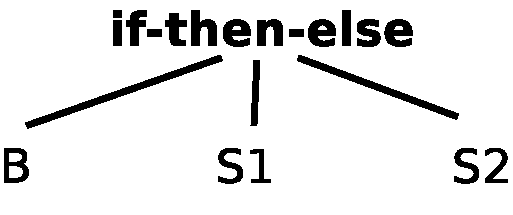
\includegraphics[width=125pt,height=53pt]{ast-ejemplo.pdf}
\caption{\label{ejem-ast} Ejemplo AST.}
\end{figure}
\begin{definition}

Dado una gramática G= \textbf{<V,T,S,P>}\, un árbol de derivación (o árbol sintáctico)
ST(G) es un árbol que se compone de dos tipos de nodos:
\begin{description}

\item [Nodos hojas] Cada nodo hoja es nombrada por una variable en T o por $\lambda$. En caso de que el nodo se nombre con $\lambda$, este es el único hijo del nodo padre.

\item [Nodos interiores] Cada nodo interior es nombrado por una variable en V. Dado $A\in V$ y $p\in P$ de la forma $A\rightarrow X_{1},X_{2},\dots, X_{k}$ el node \textbf{A} tendrá los hijos $X_{1},X_{2},\dots, X_{k}$
\end{description}
\end{definition}
\subsection*{Árbol Sintáctico atribuido}

Un árbol sintáctico atribuido es un AST que agrega información a los nodos, para almacenar los atributos de cada símbolo.
Para una mayor claridad, definimos un nodo del árbol como una tupla $( X_{0}.a_0, (X_{1}.a_1,X_{2}.a_2,\ldots ,X_{k}.a_k) )$ donde $(X_{0}.a_0)$ es el rotulo y $(X_{1}.a_1,X_{2}.a_2,\ldots ,X_{k}.a_k)$ son los nodos hijos.

Diremos que en un nodo $n=( X_{0}._{a0}, (X_{1}.a_1,X_{2}.a_2,\ldots ,X_{k}.a_k) )$ cada $X_{i}.a_i$, $(1 \leq i \leq k)$, es una instancia del atributo $X_{i}.a_i$,en la gramática.

\begin{definition} 
\label{def:ast-attr}
El árbol atribuido, sobre el cual las instancias de los atributos en cada nodo han sido definidas (es decir, cada instancia se ha asociado a un valor de su dominio), se
denomina \textbf{árbol decorado}.
\end{definition}

\begin{definition} Para un árbol sintáctico atribuido $ T(GA) $, su grafo de dependencias $ GD(T) $ es el grafo construido a partir de la composición de los grafos de dependencias $ GD(p) $ de cada producción aplicada durante la construcción de $T$. Formalmente,

$$ GD(T)=(V_{GD}(T),E_{GD}(T)) $$

donde:

\begin{enumerate}
\item $ V_{GD}(T) = \{ X.a \mid \exists n, $ un nodo de T(GA) con 
      rótulo $ X $ y $a \in A(X)$..
      
\item la relación $ E_{GD}(T) $ (arcos de $ GD(T) $) cumple con la siguiente 
      propiedad:

      Sea $n$ un nodo de $T(GA)$ con rótulo $X_0$, cuyos hijos son los nodos
      $ n_1, n_2, \ldots ,n_k $, con $ k \geq 0 $ con rótulos 
      $ X_1 $, $ X_2 $, \ldots, $ X_k $, respectivamente, y sea 
      $p:X_0 \rightarrow X_1 X_2 \ldots X_k$ una producción de GA, entonces,
      
      $$ (X_{i}.a,X_{j}.b) \in E_{GD}(T) \Leftrightarrow 
         (X_{i}.a,X_{j}.b) \in DP(p) \hspace{.5cm} 0 \leq i, \: j \leq k $$
donde DP(p) se define como:

$$ DP(p) = \{ (X_i.a,X_j.b) \mid X_j.b \rightarrow X_i.a \in R^p \} $$

\end{enumerate}
\end{definition}

\section{Métodos de Evaluación}
\label{sec:met_eval}
Un evaluador de gramáticas de atributos debe tener en cuenta las dependencias entre las instancias de atributos para seguir un orden consistente de evaluación de los mismos.
\begin{definition} Un orden de evaluación consistente, con respecto a las dependencias entre los atributos de una gramática de atributos $ GA $, es una secuencia (orden parcial) de instancias de atributos
con la siguiente restricción:

Dada una regla $r_j^p:X_0.a_0=f(\ldots,X_i.a_i,\ldots)$ en una producción $p$, 
$X_i.a_i$ deberá preceder a $X_0.a_0$.
\end{definition}

\begin{definition} Una gramática de atributos $GA$ es circular si y solo si existe un árbol sintáctico atribuido $T(GA)$, tal que su grafo de dependencias $GD(T)$ contiene al menos un ciclo.
\end{definition}

Si una GA contiene dependencias circulares no podría ser evaluada ya que no se encontraría un orden de evaluación. Esto se conoce como el problema de la circularidad, el cual se ha demostrado ser intrínsecamente exponencial\ref{XXX}. El problema de la circularidad ha motivado que muchos investigadores hayan realizado esfuerzos en la búsqueda e identificación de familias o subgrupos de gramáticas de atributos, para las cuales puedan detectarse circularidades con algoritmos de menor complejidad (polinomial o lineal).

Estas familias imponen restricciones sobre la gramática de atributos o sobre las dependencias entre sus atributos para garantizar que una GA no sea circular, con el costo de restringir su poder expresivo.

En 1980, Uwe Kastens\ref{XXX} caracterizó las gramáticas de atributos ordenadas y propuso un método para su evaluación, denominado secuencias de visita. Estas son, secuencias de operaciones que conducen el recorrido del árbol sintáctico atribuido y realizan la evaluación de las instancias de los atributos. Kastens propone un método para generar las secuencias de visita en tiempo polinomial para la familia OAG. Esta familia y otras como las absolutamente no circulares (ANCAG)\ref{XXX} son tratadas en el capítulo 2.

Luego, en 1998, Wuu-Yang en \cite{wuu-yang1} caracteriza una nueva familia denominada \textbf{Gramática de Atributos Multi-plans}, presentado una algoritmo de evaluación basado en secuencia de visita en tiempo polinomial en el numero de símbolos y producciones. Estas, son desarrolladas en el capítulo 3 y son en las que se basa el funcionamientos de \maggen.  

\subsection{Evaluación dinámica}

Un evaluador dinámico tiene como ventajas su simplicidad y que es posible evaluar cualquier WDAG (GA bien definida) o aún GA’s irrestrictas utilizando \textit{evaluación lazy}\footnote{\urllink{http://en.wikipedia.org/wiki/Lazy\_evaluation}} (siempre y cuando exista el mínimo punto fijo en el álgebra de términos denotado por las ecuaciones de atribución). Además se pueden detectar ciclos en el grafo de dependencias antes o durante la evaluación.

Las principales desventajas son que generalmente es necesario mantener el árbol sintáctico y el grafo de dependencias. La construcción del grafo de dependencias consume tiempo y memoria. Para una GA del tamaño comúnmente usado en la práctica los requerimientos de memoria pueden ser considerables.

El tiempo de procesamiento insumido en la construcción del grafo de dependencias puede ser mayor que el proceso de evaluación en sí mismo. Los evaluadores dinámicos no han tenido mucho interés en el desarrollo de herramientas de generación de procesadores de lenguajes como por ejemplo los compiladores, porque uno de los principales requisitos de un compilador es que sea eficiente, ya que durante un desarrollo un programador generalmente necesita recompilar un número muy importante de veces hasta obtener una versión final del programa requerido.

Razón por la cual en el presente trabajo se pone énfasis en métodos de evaluación estática, y no se profundizará en los métodos dinámicos

\subsection{Evaluación estática}
Los métodos estáticos deben tener en cuenta todos los posibles árboles sintácticos posibles a ser generados por la gramática y calcular todas las posibles dependencias entre las instancias de los atributos. Además, se deberán detectar las posibles dependencias circulares, para informar la viabilidad de su evaluación.

\section{Secuencia de visita}
\section{Generación de evaluadores para GA bien definidas}
\section{Evaluación durante el parsing}

bla bla

      % Introduccion.
\chapter{Clasificaci\'on de AG}
\label{chap: clas_ag}
\minitoc


bla

\section{Clasificaci\'on basada en la estrategia de evaluci\'on}

bla bla

\section{Clasificaci\'on basada en dependecias}

bla bla
\section{Clasificaci\'on de Knuth}

cla cla
\subsection{\'Arbol sint\'actico atribu\'ido}

% \begin{bulletList}
%  \item First point
%  \item Second point
% % \item Here is an abbreviation reference \nomenclature{DTI}{Diffusion Tensor Imaging} DTI
% \end{bulletList}
    % Clasificación de AG.
\chapter{Gramática de Atributos Multi-planes}
\label{chap:mag}
\minitoc

Tal como lo presenta Wuu-Yang en \cite{wuu-yang1} la familia de \textit{gramática de atributos multi-planes} es una clase que se encuentra dentro de las WDAG y dentro de ellas de las NC.

La familia de las MAG es estrictamente mayor que las ANCAG. La importancia de esta familia radica en que el procedimiento de computación de planes de evaluación estáticos toma \textbf{tiempo polinomial} en el numero de símbolos y producciones.

A continuación trataremos en detalle la familia de las MAG y en el capítulo siguiente abordaremos el mecanismo de evaluación de las mismas.

% \section{Gramática de atributos}
% En esta sección, se define la notación que se usara en le desarrollo del presente capítulo para la definición de la familia MAG.
% Básicamente, la notación usada es la utilizada por Wuu yang en \cite{wuu-yang1}, la cual proviene de la notación de Kastens en \cite{kastens}.

\section{Preliminares}
\label{sec:pre-grafos}
Antes de llegar a la definición de la familia de \textit{gramáticas multi-plans}, presentaremos un ejemplo de gramática de atributos que servirá para estudiar conceptos previos, como lo son, la construcción de una serie de grafos necesarios para el análisis de los integrantes de dicha familia.

El ejemplo es presentado en la figura \ref{ag-no-ANCAG}. El mismo es trabajo, luego, en las etapas consideradas para el diseño de \maggen.

\begin{AG}

\newproduction{S}{XYZ}
    \begin{Attribution}
        \attribution{S.s0 := f(X.s1,Y.s2,Y.s3,Z.s4)}
        \attribution{X.i1 := Y.s3}
        \attribution{Y.i2 := X.s1}
        \attribution{Y.i3 := Y.s2}
    \end{Attribution}

\newproduction{Y}{m}    
    \begin{Attribution}
        \attribution{Y.s2 := Y.i2}
        \attribution{Y.s3 := 1}
    \end{Attribution}
    
\newproduction{Y}{n}
    \begin{Attribution}
        \attribution{Y.s2 := 2}
        \attribution{Y.s3 := Y.i3}
    \end{Attribution}
    
\newproduction{X}{m}
    \begin{Attribution}
        \attribution{X.s1 := X.i1}
    \end{Attribution}
    
\newproduction{Z}{Y}
    \begin{Attribution}
        \attribution{Z.s4 := Y.s3}
        \attribution{Y.i2 := 3}
        \attribution{Y.i3 := Y.s2}
    \end{Attribution}
\caption{Una gramática de atributos no ANCAG}
\label{ag-no-ANCAG}
\end{AG}
\subsection{Grafo \textit{DP}}
Los grafos \textit{DP} denotan las relaciones de dependencias directas entre las instancias de la gramática. 

Un grafo \textit{DP} esta definido (\cite{estruc-algorit}) con las siguientes consideraciones: 

\begin{itemize}
\item Los nodos denotan \textit{instancias} de una producción.
\item Las aristas denotan la dependencia entre las instancias. Una arista $X_{i}.a\rightarrow X{j}.b$, \footnote{con \textit{i} y \textit{j} índices de ocurrencias consistentes con alguna ecuación de la gramática} denota que la evaluación de la instancia \textit{$X_{i}.a$} depende de la evaluación de \textit{$Y_{i}.b$} 
\end{itemize}

El conjunto de dependencias directas de una producción, de la gramática, se denota como \textit{DP(p)}(\textit{p} producción de la gramática) y se define como:
\begin{definition}
Dada una producción p de una gramática de atributos definida como en \ref{def:grammarattr}, entonces
\begin{equation}
DP(p) = \{(X_{i}.a, X_{j}.b) | X_{i}.a \rightarrow Y_{j}.b \in R^{p} \}
\end{equation}
\end{definition}

La noción de dependencia directa y DP(p) fueron presentados, también, en el capítulo introductorio, cuando se presentó la definición de Árbol sintáctico atribuido (\label{def:ast-attr}).  
En la figura \ref{dp-wuu-yang} se observan los grafos DP para la gramática de la figura \ref{ag-no-ANCAG}.

\subsection{Grafo \textit{Down}}
Los grafos \textit{Down} denotan las relaciones de los atributos de un símbolo. 

Un grafo \textit{Down} esta definido (\cite{estruc-algorit}) con las siguientes consideraciones: 

\begin{itemize}
\item Los nodos denotan \textit{atributos} de un símbolo.
\item Las aristas denotan la dependencia entre los atributos de un símbolo. Dado los atributos $a$ y $b\in A(X)$ del símbolo $X\in VN$, una arista $a\rightarrow b$, denota que la evaluación del atributo \texttt{a} depende de la evaluación de \texttt{b}. 
\end{itemize}
El conjunto de dependencias entre los atributos de un símbolo se denota como  
\texttt{Down(X)}($X\in VN$ de una gramática G) y se define:
\begin{definition}
Dada un símbolo X de una gramática de atributos definida como en \ref{def:grammarattr}, entonces
\begin{equation}
Down(X) = \{(a,b) | a \rightarrow b \} con\ a,b \in A(X)
\end{equation}
\end{definition}
En la figura \ref{down-wuu-yang} se muestran los grafos Down(X) y Down(Y) para la gramática de la figura \ref{ag-no-ANCAG}.

\subsection{Grafo \textit{DCG}}

\textit{DCG} significa \textit{Downward Characteristic Graphs}, los mismos contienen las dependencias entre instancias de la gramática para una producción \textit{p}, teniendo en cuenta un símbolo en la gramática.
\begin{definition}
Dado q una producción de la forma $X_{0}\rightarrow \alpha_{0} X_{1} \alpha_{1} X_{2} \dots X_{k} \alpha_{k}$, el \textit{Downward Characteristic graph} of $X_{0}$ en los subárboles derivados vía la producción \textit{q}, denotado como $DCG_{X_{0}}(q)$, es un grafo donde: 
\begin{itemize}
\item Los nodos son atributos del símbolo $X_{0}$.
\item Una arista, $X.a \rightarrow X.b$, denota una dependencia (transitiva) de X.b sobre X.a en algún subárbol derivado desde $X_{0}$ vía \textit{q}.
\end{itemize}
\end{definition}
Tomemos el siguiente teorema presentado por Wuu-Yang en \cite{wuu-yang1}:
\begin{theorem}
$\bigcup\limits_{\textit{todo p}}{DCG_{X} (p) = Down (X)}$
\end{theorem}
\underline{Nota:} $DCG_{X}(p)$ contiene las dependencias, entre las instancias de la gramática, para el símbolo \texttt{X}, acotando el análisis para la producción \textit{p} y los posibles contextos inferiores.

En la sección \ref{XXX} se analiza el algoritmo para construir los grafos DCG.

\subsection{Grafo \textit{ADP}}

Las siglas \textit{ADP} significan \textit{Augmented Dependency graph}. El grafo \textit{ADP} esta definido por instancias de la gramática, en los nodos, y cada arista se define como: $X_{i}.a\rightarrow X{j}.b$, denota que la evaluación de la instancia \textit{$X_{i}.a$} depende de la evaluación de \textit{$Y_{i}.b$}.

El conjunto de dependencias aumentadas se denota como $ADP (q | p_{1}, p_{2}, \dots, p_{k})$ y se define:
\begin{definition}
Sea q una producción de la forma $X_{0}\rightarrow \alpha_{0} X_{1} \alpha_{1} X_{2} \dots X_{k} \alpha_{k}$. Sea $p_{i}$ una producción cuya parte izquierda es $X_{i}$ ($1\leqslant i \leqslant k$). 
\begin{equation}
ADP (q | p_{1}, p_{2}, \dots, p_{k}) = DP(q) \bigcup\limits_{k}^{i=1}{DGC_{X_{i}}} (p_{i})
\end{equation}
\end{definition}

A partir de la definición anterior surge la siguiente:
\begin{definition}
El conjunto de todas las posibles dependencias aumentadas para una producción q se define como:
\begin{equation}
SADP(q) = \bigcup\limits_{q\in P}{ADP (q | p_{1}, p_{2}, \dots, p_{k})} 
\end{equation}
\end{definition}

\begin{figure}\centering
 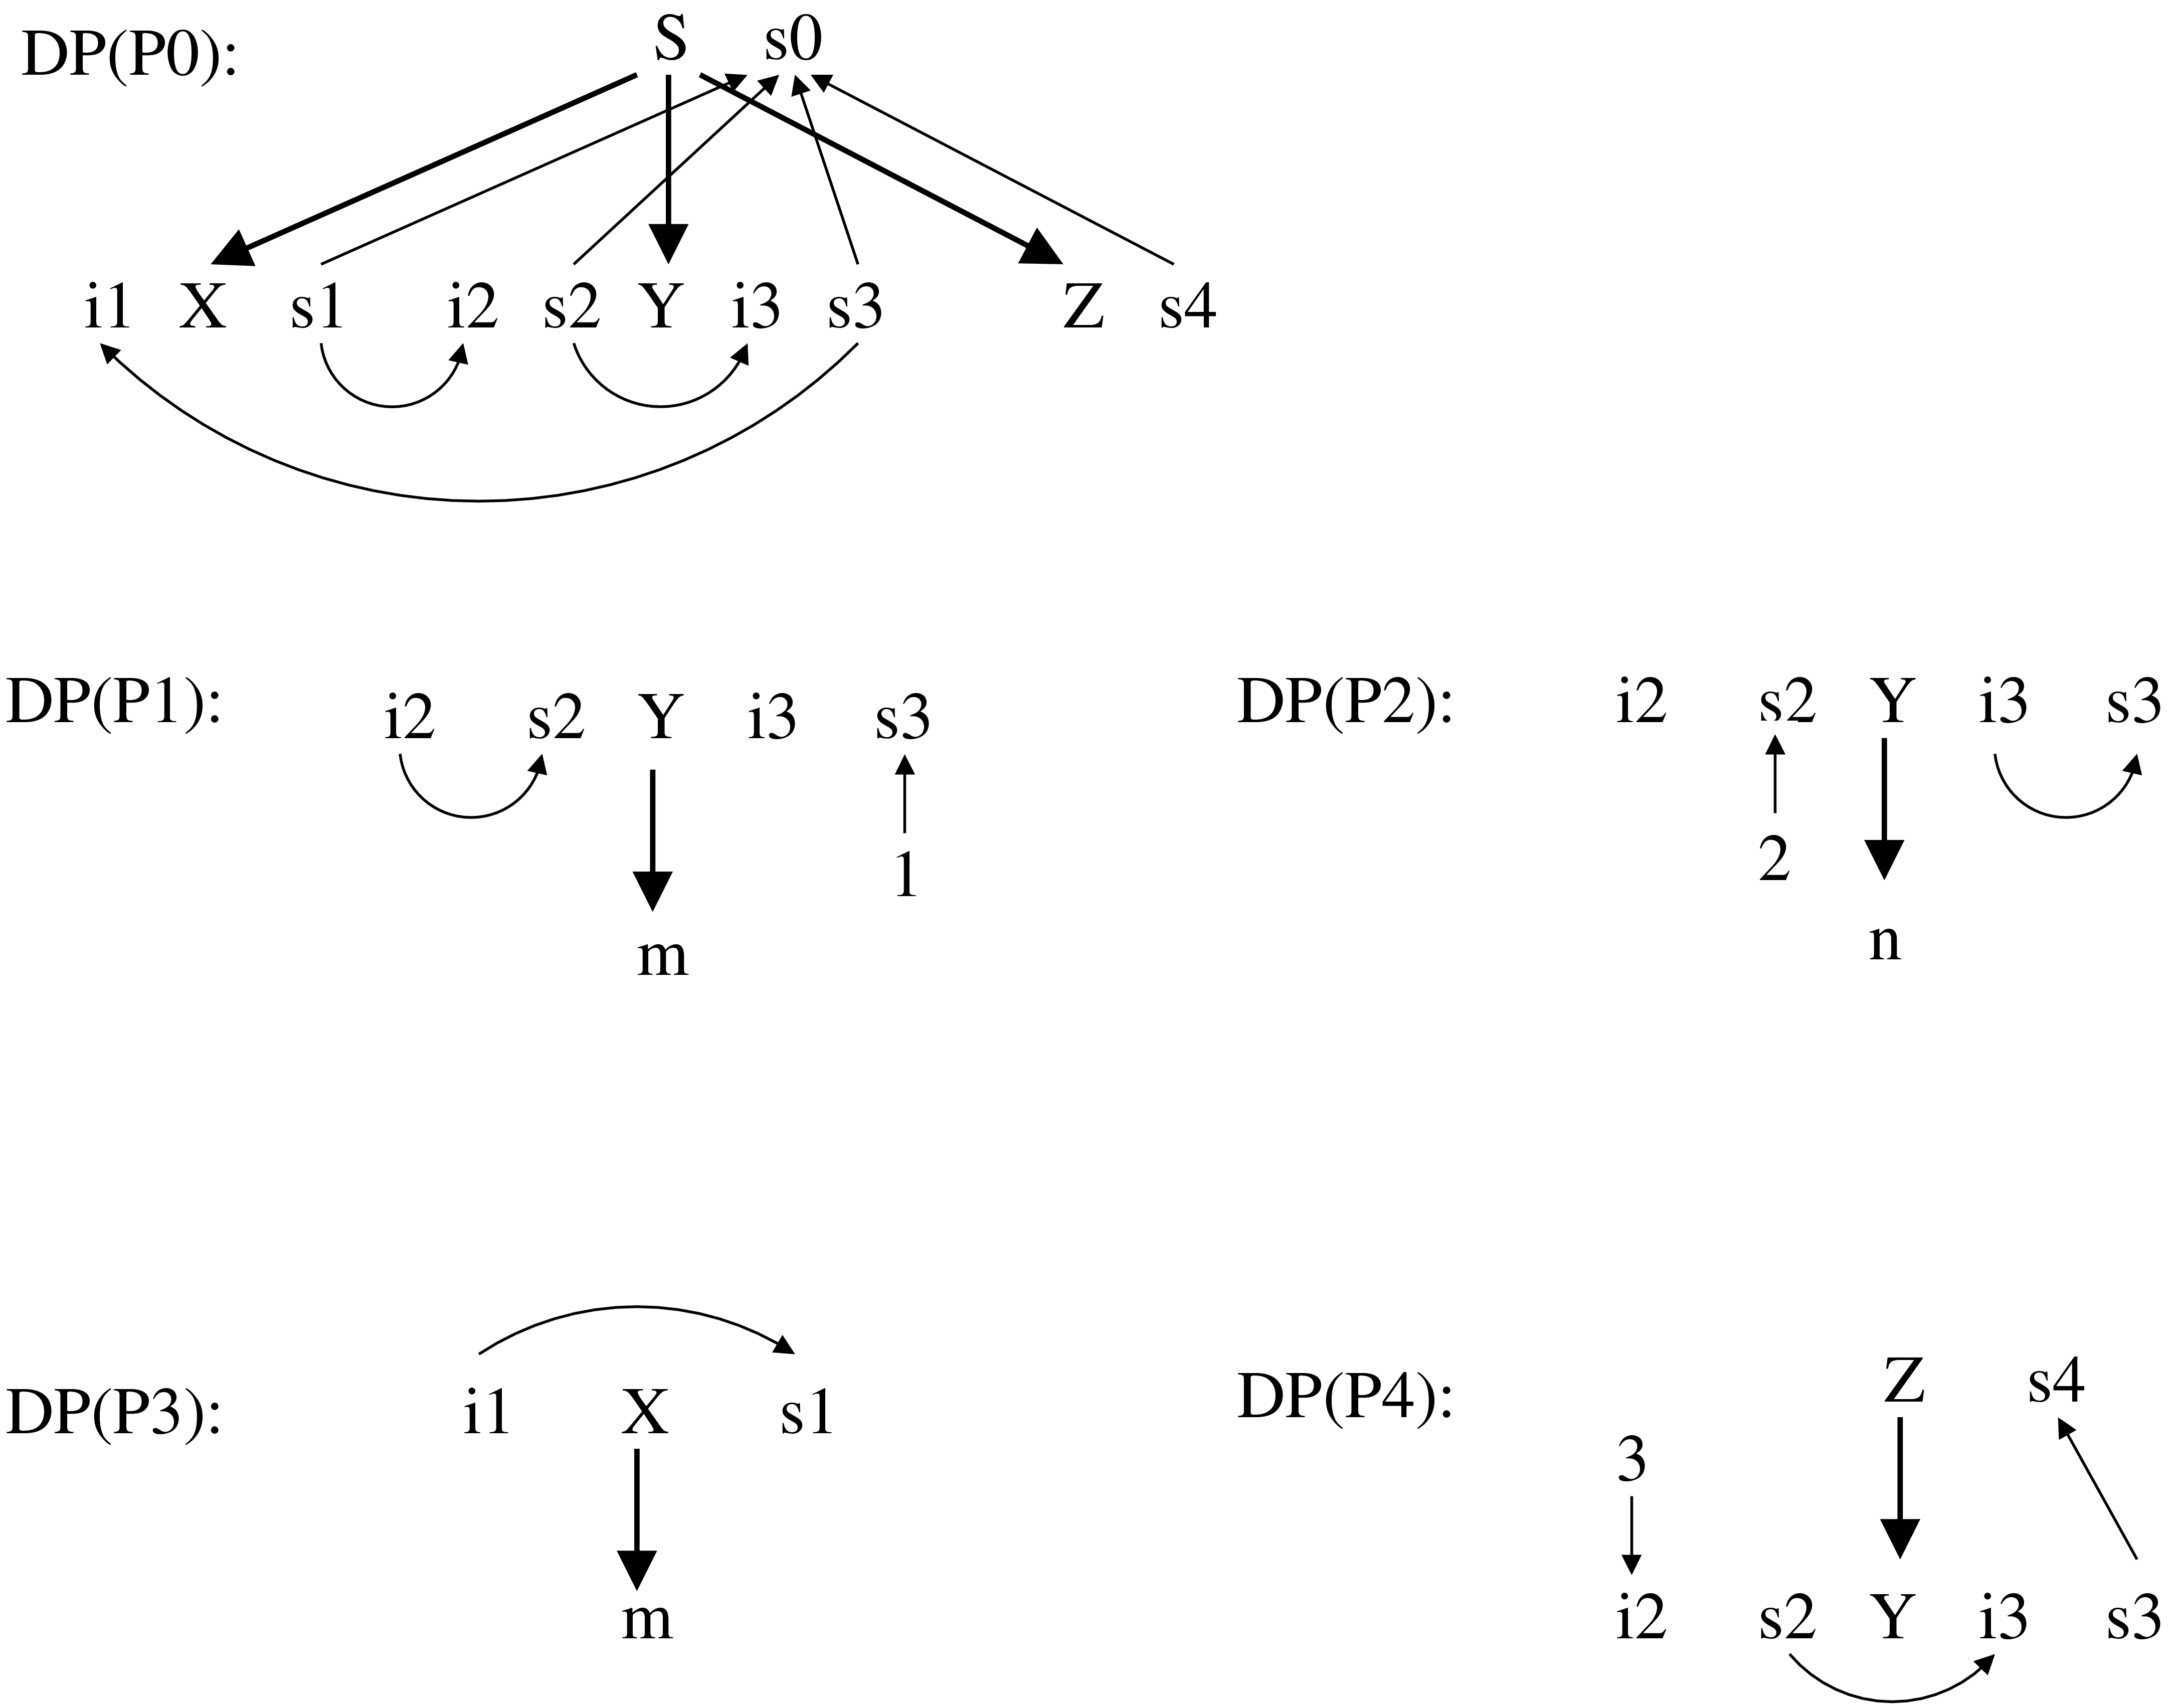
\includegraphics[width=250pt,height=195pt]{ej-grafos.png}
\caption{\label{dp-wuu-yang}Grafos DP para la gramática de la figura \ref{ag-no-ANCAG}.}
\end{figure}
\begin{figure}\centering
 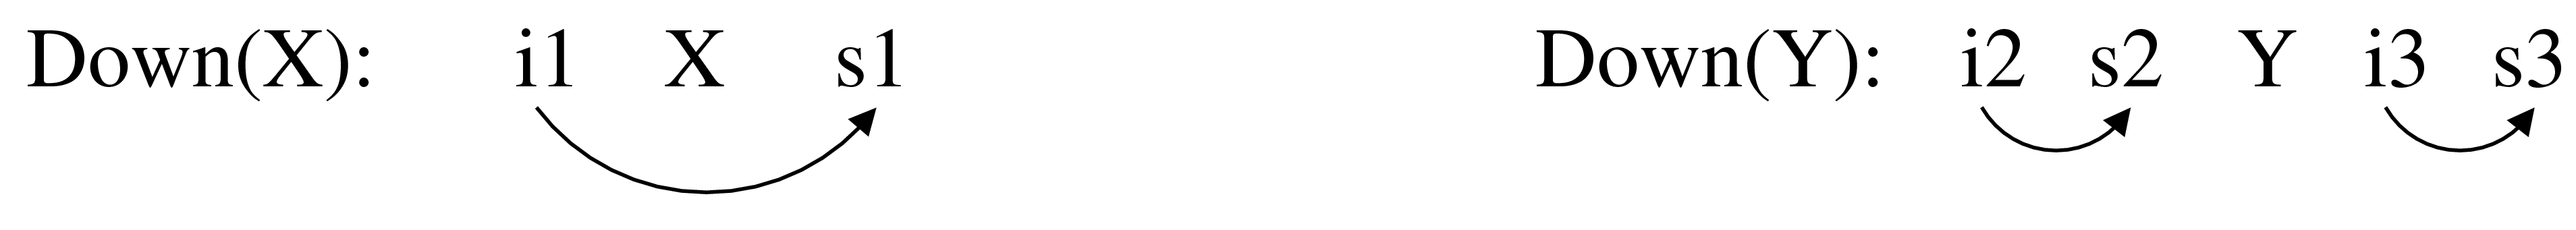
\includegraphics[width=350pt,height=31pt]{ej-grafos1.png}
\caption{\label{down-wuu-yang} DOWN(X) y DOWN(Y) para la gramática de la figura \ref{ag-no-ANCAG}.}
\end{figure}

\begin{figure}\centering
 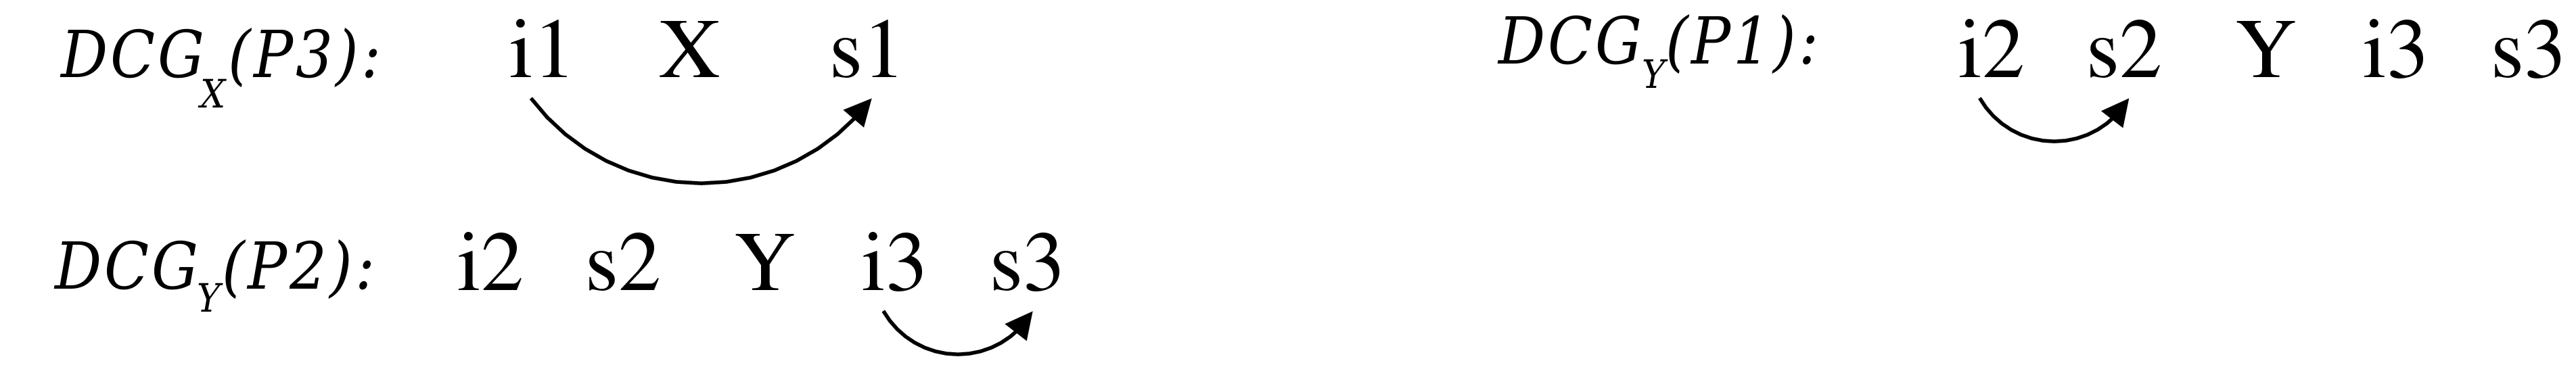
\includegraphics[width=350pt,height=52pt]{ej-grafos3.png}
\caption{\label{dcg-wuu-yang} Grafos DCG para la gramática de la figura \ref{ag-no-ANCAG}.}
\end{figure}

\begin{figure}\centering
 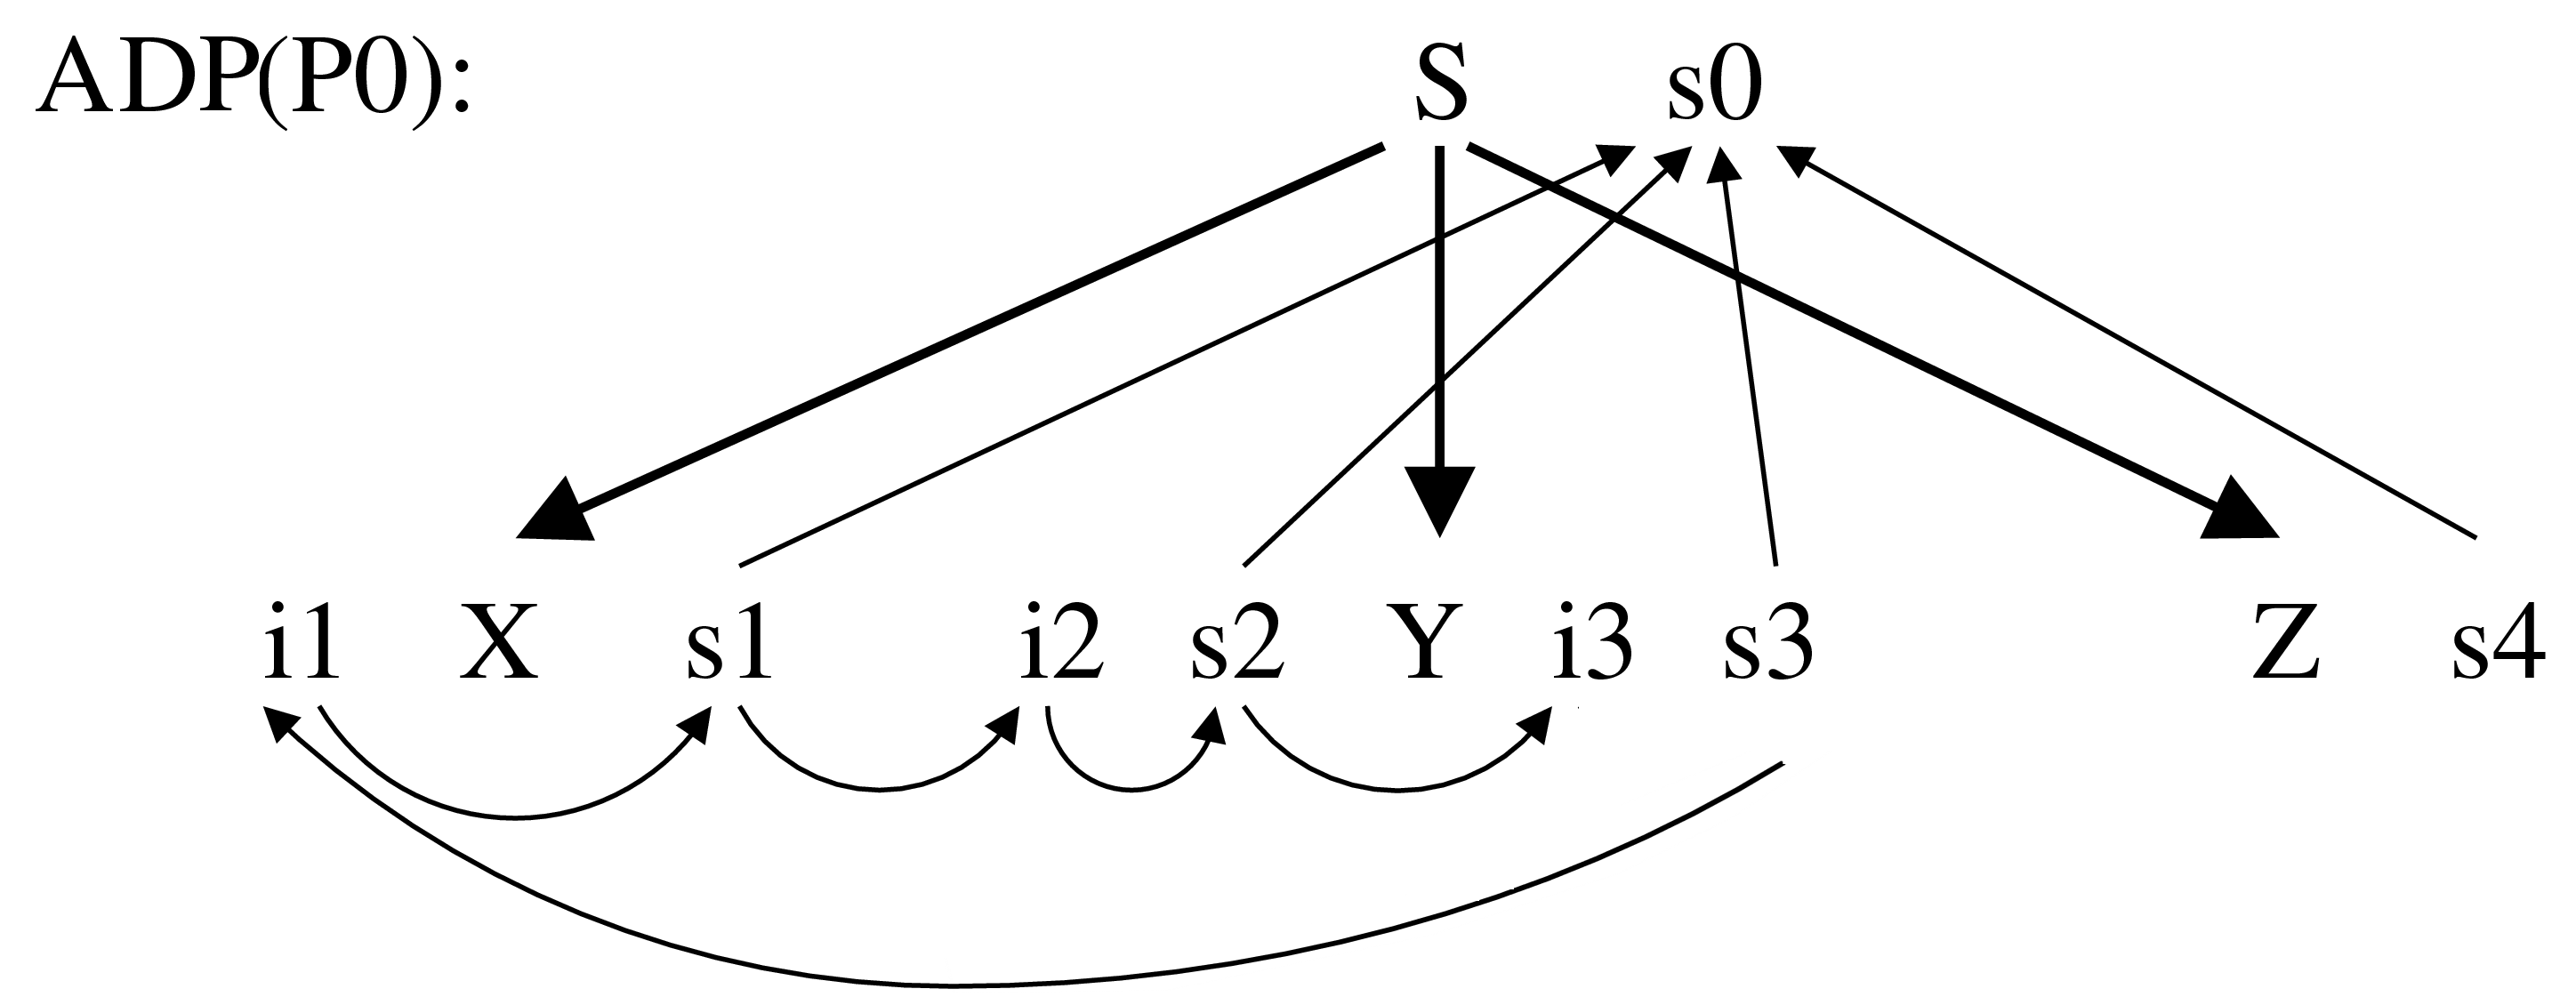
\includegraphics[width=350pt,height=132pt]{ej-grafos4.png}
\caption{\label{adp-wuu-yang} ADP(P0):contexto inferior P1, para la gramática de la figura \ref{ag-no-ANCAG}.}
\end{figure}

\section{Definición MAG}

Una gramática \textit{G} de la forma \ref{def:grammarattr} es una \textit{gramática de atributos multi-planes} si y solo si 
\begin{equation}
\forall q : q \in P: (\forall g:g\ es\ un\ grafo\ de\ q \wedge g \in SADP(q) : g\ es\ no\ circular) 
\end{equation}

Las \textit{gramáticas multi-plans} mantienen propiedades deseables como:
\begin{itemize}
\item La clases de gramáticas MAG cumplen la propiedad de que todas las gramáticas de atributos en dicha clase son \textbf{no circulares}.
\item Toda gramática MAG cumple con las propiedades de gramática bien definida, esto es, todo árbol sintáctico derivado sobre una MAG contiene dependencias no circulares.
\end{itemize}


De los conceptos analizado arriba surgen la siguiente definición y los siguientes 2 teoremas:

\begin{definition}
 Sea una \textit{q} una producción de la forma $X_{0}\rightarrow \alpha_{0} X_{1} \alpha_{1} X_{2} \dots X_{k} \alpha_{k}$. Sea $p_{i}$ definimos:
\begin{equation}
 IDP-ANCAG(q) = DP(q) \bigcup\limits_{k}^{i=1}{Down(X_{i})}
\end{equation}

\end{definition}

\begin{theorem}
$IDP-ANCAG(q) = \bigcup SADP(q)$, para toda producción q. 
\end{theorem}

\begin{theorem}
Toda gramática ANCAG es una gramática MAG, pero no viceversa.
\end{theorem}

\begin{figure}\centering
 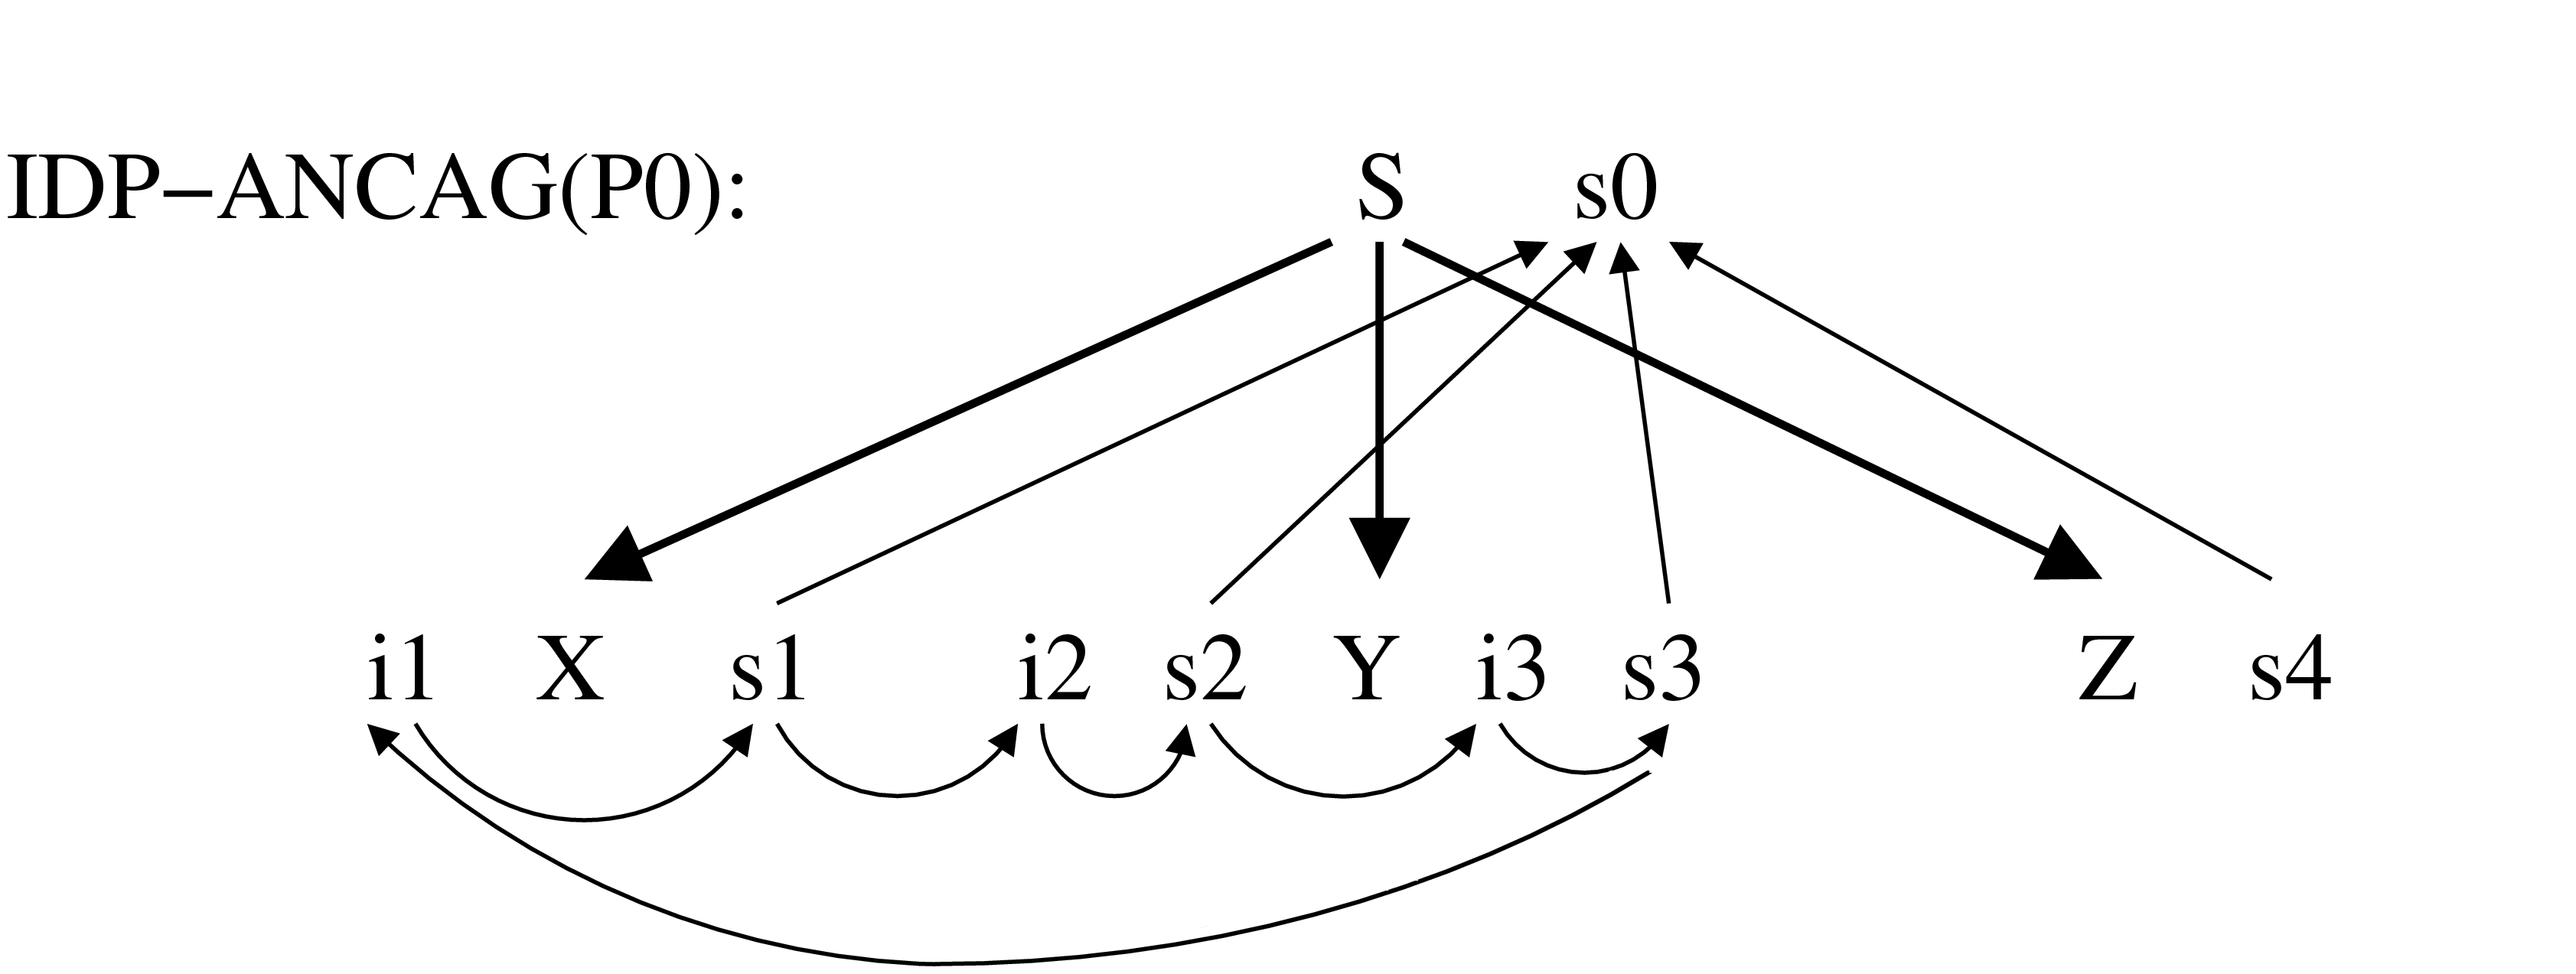
\includegraphics[width=350pt,height=132pt]{ej-grafos2.png}
\caption{\label{idp-wuu-yang}Grafo IDP-ANCAG(P0) para el ejemplo \ref{ag-no-ANCAG}.}
\end{figure}

Un resultado que muestra la veracidad del teorema anterior se observa en la gramática de la figura \ref{ag-no-ANCAG}, la cual es gramática MAG, pero la misma no es ANCAG. Este resultado se puede notar en la figura \ref{ancag-circle}, donde se marca la dependencia circular en el grafo.
\begin{figure}\centering
 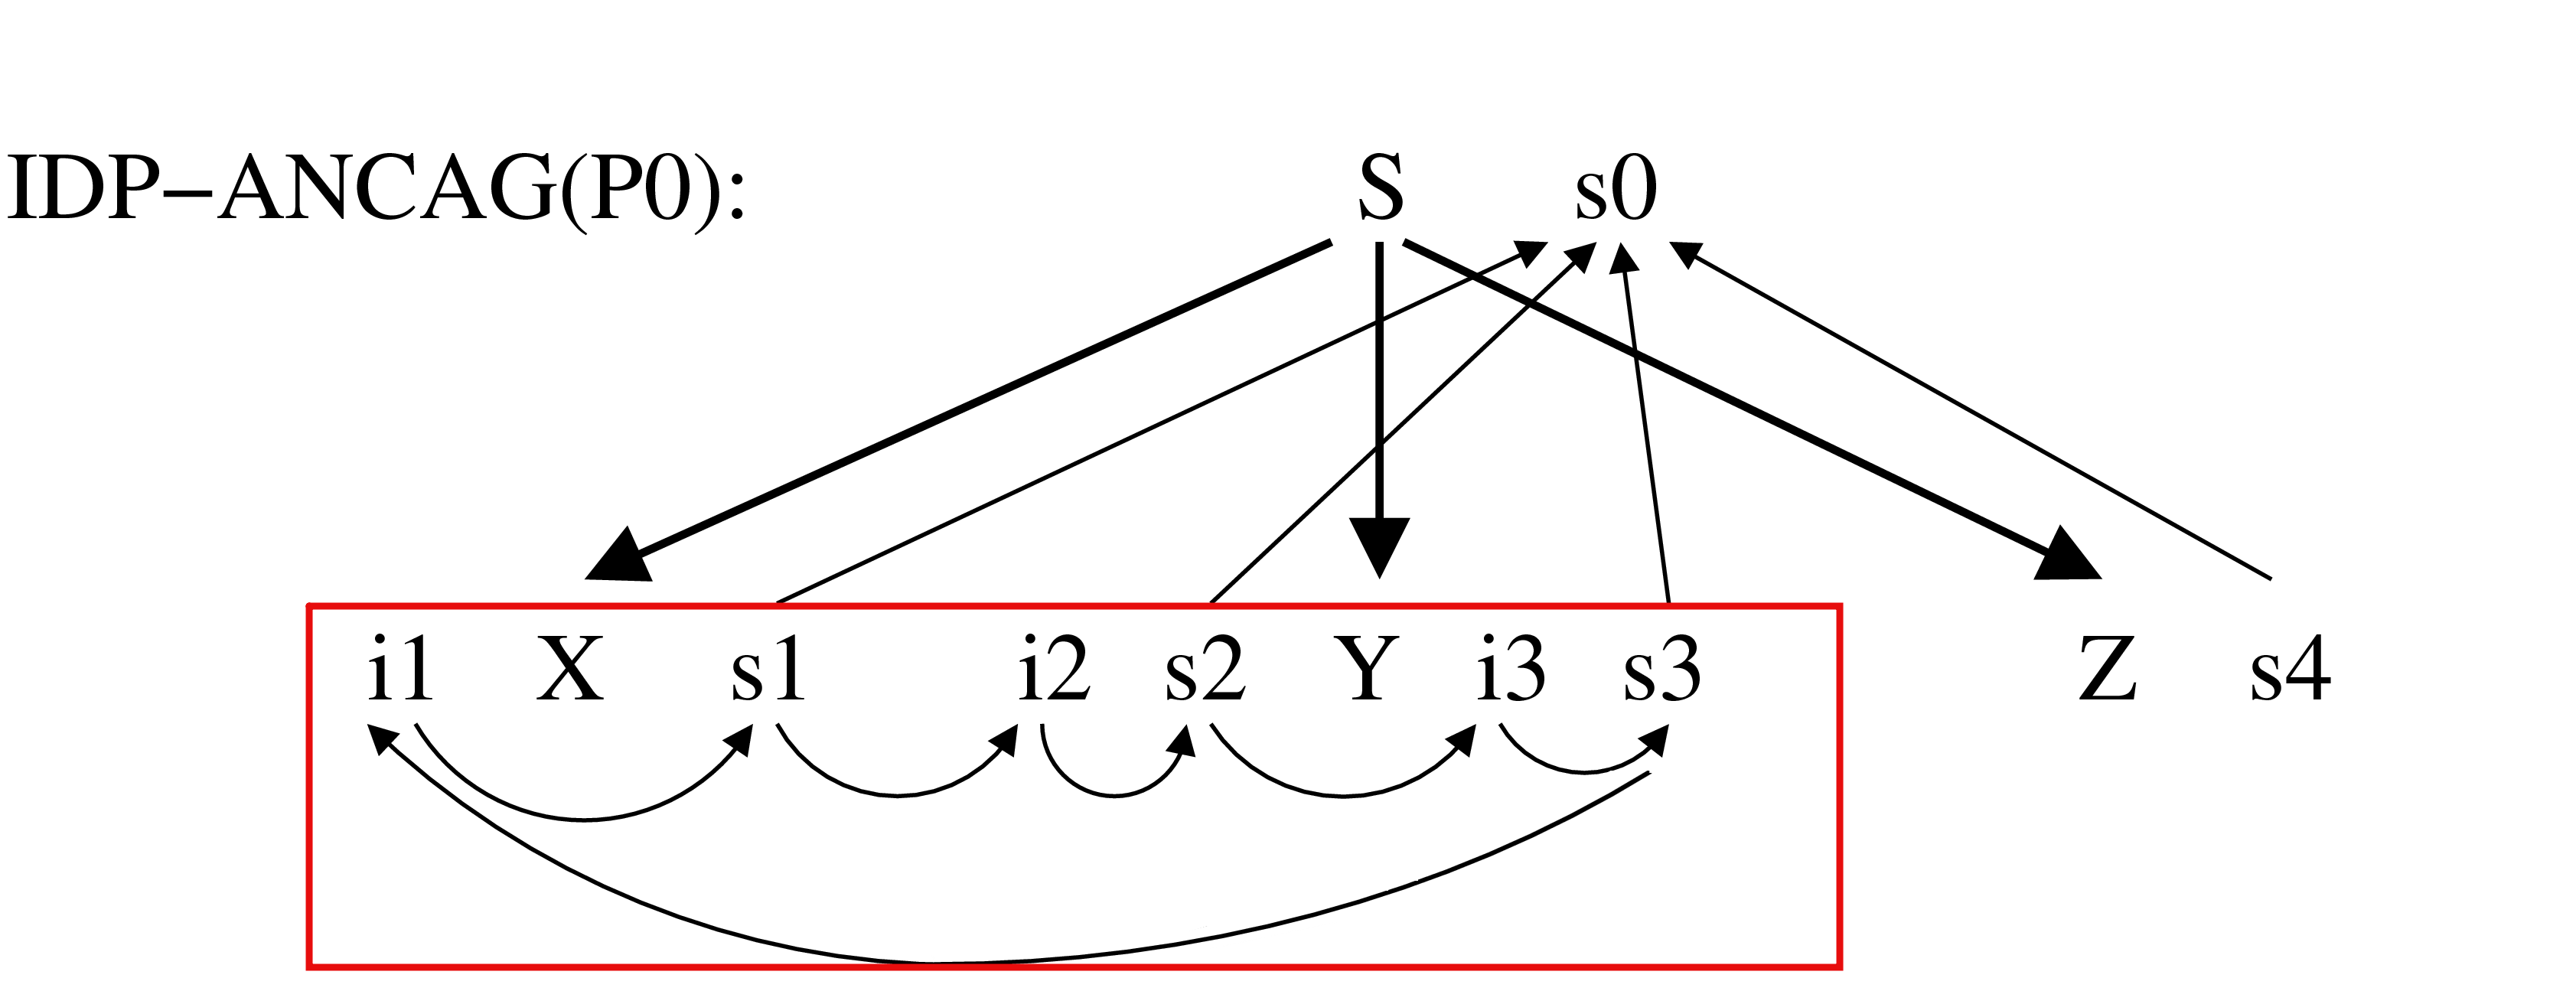
\includegraphics[width=350pt,height=135pt]{ej-grafos2-circle.png}
\caption{\label{ancag-circle} Grafo IDP-ANCAG(P0) marcando ciclo.}
\end{figure}
        % Gramáticas de atributos multiplanes.
\chapter{Evaluación estática de MAG}
\label{chap:eval_est}
\minitoc

En este capítulo se presentan los algoritmos de construcción de cada tipo de grafo, así como los usados para el cómputo de planes de evaluación y sus respectivas secuencias de visita. Los mismos se basan en los propuestos por Wuu Yang en \cite{wuu-yang1}. Mientras que el algoritmo para el cálculo de secuencias de visita fue íntegramente desarrollado e implementado en el marco de la tesis.

Para comprobar la correctitud de los algoritmos y lograr mayor grado de eficiencia, los mismos fueron testeados mediante la herramienta \textit{gcov}\footnote{Detalles en sección \ref{sec:metoherram}.}. La cual fue utilizada con mayor énfasis para el algoritmo de cómputo de secuencias de visita. En conjunto con los resultados proporcionados por \textit{gcov} y análisis teóricos, la heurística que implementa el algoritmo fue refinada en varias oportunidades.

\section{Algoritmos para cómputo de grafos}

Todos estos algoritmos tienen una característica en común, expresan las dependencias existentes entre los atributos de una gramática desde distinto aspectos. Por lo tanto en su construcción, los nodos y aristas son obtenidos de las relaciones entre dichos elementos.

\subsection{Cómputo de DP}
\label{subsec:alg-DP}
Se debe generar un grafo DP por cada regla de la gramática, representando las dependencias directas entre los atributos de los símbolos que participan en la producción, tal como se analizó en el capítulo anterior en la sección \ref{subsec:graph-dp-def}.

Es el más directo de construir, ya que por cada ecuación de la regla actual, se agrega una arista entre cada uno de los símbolos de \textbtt{r\_value} con destino al \textbtt{l\_value} de la ecuación. Obviamente se deben agregar los nodos necesarios y sin repeticiones, para cada una de las instancias de atributos. Ver algoritmo \ref{alg:graphdp}.

\begin{algorithm}[!ht]
\lstinputlisting[language=specmag, numbers=left, columns=fullflexible]{input_file_code/compute_dp_wuu_yang}
\caption{\label{alg:graphdp} Cómputo de grafos \textit{DP}}
\end{algorithm}

\subsection{Cómputo de Down}
\label{subsec:alg-DOWN}
Este tipo de grafo, se debe crear para cada uno de los símbolos no terminales de la gramática. Representan las relaciones de dependencia entre solamente sus atributos, considerando todas las reglas en las que participan (Ver sección \ref{subsec:graph-down-def} del capítulo anterior). Para más detalle, ver algoritmo \ref{alg:graphdown}.

\begin{algorithm}[!ht]
\lstinputlisting[language=specmag, numbers=left, columns=fullflexible]{input_file_code/compute_down_wuu_yang}
\caption{\label{alg:graphdown} Cómputo de grafos \textit{Down}}
\end{algorithm}

La función \textbtt{project} recibe un grafo, del cual debe eliminar todos los nodos y aristas relacionadas que no pertenecen al conjunto de atributos que le pasan como segundo parámetro. Pero para evitar que al eliminar nodos y aristas el grafo pierda información sobre las dependencias entre los atributos, se calcula previamente la clausura transitiva del grafo. La implementación de \textbtt{project} se presenta en el algoritmo \ref{alg:graphproj}.

\begin{algorithm}[!ht]
\lstinputlisting[language=specmag, numbers=left, columns=fullflexible]{input_file_code/project_wuu_yang}
\caption{\label{alg:graphproj} Proyección sobre grafos}
\end{algorithm}

\subsection{Cómputo de DCG}
\label{subsec:alg-DCG}
Estos grafos se generan para cada regla de la gramática y considerando las dependencias entre los atributos del símbolo de la parte izquierda de la producción (\textbtt{head}). Para computarlo, tal como se lo definió en la sección \ref{subsec:graph-dcg-def}, se deben unir el grafo \textit{DP} de la regla junto a todos los grafos \textit{Down} de los símbolos de la parte derecha de la regla (\textbtt{body}) y luego se utiliza, nuevamente, la función \textbtt{project}. Para más detalle, ver algoritmo \ref{alg:graphdcg}.

\begin{algorithm}[!ht]
\lstinputlisting[language=specmag, numbers=left, columns=fullflexible]{input_file_code/compute_dcg_wuu_yang}
\caption{\label{alg:graphdcg} Cómputo de grafos \textit{DCG}}
\end{algorithm}

\subsection{Cómputo de ADP}
\label{subsec:alg-ADP} 
Para generar estos grafos, Wuu Yang no plantea un algoritmo preciso aunque no es necesario ya que toda la heurística necesaria se encuentra en la definición de los mismos (ver \ref{mag:adpdef}).

Un grafo ADP corresponde a una regla bajo una cierta combinación de producciones para cada uno de sus hijos. Es decir, que para una misma regla pueden existir varios grafos ADP, ya que sus hijos pueden producir más de un contexto. El cómputo de grafos ADP es presentado en el algoritmo \ref{alg:graphadp}.

\begin{algorithm}[!ht]
\lstinputlisting[language=specmag, numbers=left, columns=fullflexible]{input_file_code/compute_adp_wuu_yang}
\caption{\label{alg:graphadp} Cómputo de grafos \textit{ADP}}
\end{algorithm}

\section{Algoritmo de cómputo de planes}
\label{sec:comp-planes}
Luego de verificar que la gramática es MAG\footnote{Ver \ref{def:MAG}.}, se deben generar los planes de evaluación para la gramática. Cada ADP producirá un plan de evaluación, por lo que ambos tendrán el mismo identificador, es decir, la regla a la cual pertenecen y el contexto que se aplicó a los símbolos no terminales de la misma.

Este algoritmo propuesto por Wuu Yang, es detallado en profundidad en esta sección y la correctitud del algoritmo es abordado por Wuu Yang en \cite{wuu-yang1}.

La idea principal es utilizar una cola de trabajos, en la cual se insertan pares que contienen una regla y un orden de evaluación para sus instancias. Para cada uno de los grafos ADP asociados a la regla, se le computa su orden de evaluación para el contexto especificado por el grafo.

Luego, para cada uno de los símbolos no terminales de la parte derecha de la regla, considerando la producción que le corresponde según el contexto, se obtiene el plan proyectado. Ese nuevo par, se intenta insertar en la cola de trabajos para seguir con el cómputo de planes (Ver algoritmo \ref{alg:planeval}).

\begin{algorithm}[!ht]
\lstinputlisting[language=specmag, numbers=left, columns=fullflexible]{input_file_code/compute_plan_wuu_yang}
\caption{\label{alg:planeval} Cómputo de planes de evaluación}
\end{algorithm}

La función \textbtt{compute\_order}, debe agregarle al grafo ADP la información inducida por el orden para evaluar los atributos del símbolo \textbf{head} de la regla a la que pertenece el grafo.

Para ello, como todo orden se puede ver como una secuencia, se agregan al grafo un nodo por cada elementos del orden y las aristas para todos los pares posibles\footnote{Ver más detalles en \ref{sec:genplanes}} (Ver algoritmo \ref{alg:compord}).

\begin{algorithm}[!ht]
\lstinputlisting[language=specmag, numbers=left, columns=fullflexible]{input_file_code/compute_order_wuu_yang}
\caption{\label{alg:compord}Cómputo de orden de evaluación}
\end{algorithm}

La funcionalidad que cumple \textbtt{project} (en el cómputo de planes), es dado un orden de evaluación purgarlo de todo elemento ajeno a el conjunto de ocurrencias de atributos especificados como parámetro. Previamente se debe aplicarle la clausura transitiva para conservar las relaciones de precedencia entre las ocurrencias (Ver algoritmo \ref{alg:projordeval}).

\begin{algorithm}[!ht]
\lstinputlisting[language=specmag, numbers=left, columns=fullflexible]{input_file_code/project2_wuu_yang}
\caption{\label{alg:projordeval} Proyección sobre orden de evaluación}
\end{algorithm}

Un resultado muy importante a tener en cuenta es el echo de que el algoritmo \ref{alg:planeval} genera la minima cantidad de planes que son necesarios para la evaluacion de una gramatica.

Este resultado es expresado mediante un teorema (teorema \ref{teo:planes_plausibles}), pero antes de llegar al mismo es recomendable tener en cuenta algunos aspectos y definiciones.

En primer lugar, en todo grafo ADP se almacenan las dependencias entre instancias de atributos, segun; las \textit{dependencias directas}, las dependencias impuestas por el \textit{contexto superior} y las del \textit{contexto inferior}. Entonces, instancias diferentes de una producción $p$ tendrán las mismas dependencias directas (Grafo DP), pero podrán tener diferentes dependencias impuestas por los contextos inferiores y superiores. Estas, y demás observaciones deben tenerse en cuenta para la construcción de un plan de evaluacion. En consecuencia, es necesario determinar todas las \emph{dependencias posibles} entre las instancias de los atributos que ocurren en una producción para luego poder determinar todas las \emph{dependencias plausibles} entre los atributos que ocurren en una producción. 

\begin{definition} Una partición posible de un grafo de dependencias $G\_T=<V\_N,A>$ es una partición sobre $V\_N$ tal que dados dos instancias de atributos $X.a$ y $Y.b$, si $(X.a,Y.b) \in A$, entonces $[X.a] = [X.b]$ (están en la misma clase).
\end{definition}

\begin{definition} Sea $\pi$ una partición posible de un grafo de dependencias $G_T=<V_N,A>$. Sea $V_{N_X}$ un nodo rotulado $X$ en el árbol sintáctico $T$. La proyección de $\pi$ en las instancias de los atributos de $X$ es una partición posible de los atributos de $X$.
\end{definition}

Una \textit{partición plausible} es un refinamiento de una partición posible, dado que las restricciones impuestas por algún contexto superior puede que dos clases de una partición plausible se unan en una partición posible (en el caso de una dependencia transitiva entre dos instancias de atributos impuesta por el contexto superior). Para el símbolo de comienzo la partición plausible coincide con una partición posible (ya que no tiene contexto superior). \\


\begin{definition}
\label{def:plan_espurios}
Dada una MAG, se define \textbf{plan espurio} a aquel plan de evaluación para el cual no es posible encontrar un AST para dicho plan.

NOTA: podriamos ver como: proviene de una particion posible que no puede ser plausible.
\end{definition}

\begin{definition}
\label{def:plan_plausible}
Dada una MAG, se define \textbf{plan plausible} a aquel plan de evaluación para el cual existe al menos un AST para dicho plan.

NOTA: lo podriamos ver como: un plan es plausible si proviene de la union de particiones plausibles.
\end{definition}


\subsection{Teorema}
\label{teo:planes_plausibles}
El algoritmo \ref{alg:planeval} genera la minima cantidad de planes o dicho en otras palabras, genera solamente planes plausibles.

\underline{\emph{Demostración:}}


\section{Algoritmo de cómputo de secuencias de visita}
\label{sec:algseqvisit}

Las secuencias de visitas, son traducciones de los planes de evaluación en secuencias compuestas por tres comandos\footnote{\textbtt{compute}, \textbtt{leave} y \textbtt{visit}, ver más detalles en \ref{sec:sec-visit}.} que permiten la navegación por el AST para su evaluación.

Este proceso fue diseñado e implementado para el desarrollo de \maggen. La generación se dividió en dos algoritmos, uno encargado de la inicialización de todas las secuencias de visitas y la invocación del otro, solamente, para los planes de evaluación que pertenecen a la producción inicial de la gramática. Este último algoritmo calcula las secuencias de visitas totales.

La traducción bajo demanda de los planes de evaluación, permiten realizar optimizaciones como se explicará en el capítulo \ref{chap:implem} de implementación. El cómputo de secuencias de visita es presentado en el algoritmo \ref{alg:genvisitseq}.

\begin{algorithm}[!ht]
\lstinputlisting[language=specmag, numbers=left, columns=fullflexible]{input_file_code/generate_visit_sequences}
\caption{\label{alg:genvisitseq} Generador de secuencias de visitas}
\end{algorithm}

El algoritmo que realiza el cómputo de las secuencias de visita totales realiza un proceso recursivo para lograr la traducción. Se lo puede considerar como una simulación del recorrido sobre el árbol en tiempo de evaluación \footnote{En la sección \ref{sec:constseqvisit} se ampliará este funcionamiento.}. Por lo que se debe llevar una secuencia de visita local, a la cual se le insertarán los distintos comandos. Además, será necesario una función que lleve las instancias de atributos ya calculadas.

De esta forma, cuando se detecta un \textbtt{visit}, se debe localizar a que hijo tiene que recursar en base al plan actual, el cual tiene un contexto establecido. Además se debe determinar el plan proyectado que actuará de orden de evaluación impuesto en la recursión. Al volver se debe actualizar todas las instancias de atributos que fueron computadas en el contexto inferior, para evitar futuras visitas innecesarias.

Con el mismo criterio, al producirse un \textbtt{leave} por la necesidad de requerir que en el contexto superior se calcule una instancia de atributo, puede ser que se calculen más de lo que solicitó, por eso se deben actualizar la información de computados.

Una ecuación se podrá computar solamente cuando todo su \textbtt{r\_value} halla sido marcado como computado, ya sea mediante un \textbtt{visit} o \textbtt{leave}.

Por último, es necesario una función que combine y actualice la secuencia de visita global, con la que se calculó a nivel local. Esto es, ya que, una secuencia de visita puede ser completada en más de una visita. Todo el proceso analizado anteriormente es presentado en el algoritmo \ref{alg:genvisitseqrec}.

\begin{algorithm}[!ht]
\lstinputlisting[language=specmag, numbers=left, columns=fullflexible]{input_file_code/gen_visit_seq}
\caption{\label{alg:genvisitseqrec} Función recursiva de generación de secuencias de visita}
\end{algorithm}

\section{Algoritmo de evaluación de atributos}
\label{sec:algevalattr}

Este algoritmo, no se encuentra implementado dentro de \maggen, sino que dentro del código del evaluador generado.

Se basa en dos etapas bien definidas y con propósitos diferentes. En las cuales se deben realizar dos recorridos del AST de entrada.

El primero es una barrida descendente en la que se seleccionan los planes de evaluación para cada nodo, para lo cual se debe armar su contexto en base a la regla referenciada por el nodo actual y la que poseen cada uno de sus hijos. El orden de evaluación de atributos para la raíz del AST es aleatoria, ya que sólo contiene símbolos sintetizados y no pueden ser utilizados en otro contexto por ser una gramática extendida.

En el segundo recorrido, no precisamente se realiza en un sentido uniforme, sino que se navega descendente y ascendentemente, de acuerdo a la secuencia de visita correspondiente al plan seleccionado en la primera etapa. 

La primera etapa es realizada en la funcion \textbtt{traverse}. Esta, tiene toda la información necesaria ya precargada, gracias al procesamiento previo de los anteriores algoritmos. Debe determinar el plan de evaluación, almacenado en $\Gamma$, armando la clave con la regla asociada al nodo corriente y las reglas asociadas de todos los hijos. El orden de evaluación de atributos $\omega$, le viene como parámetro, el cual corresponde con un plan de evaluación proyectado, que desde el contexto superior le impusieron. Una vez seleccionado el plan, también queda establecida la secuencia de visita, para el nodo.

Para continuar con el proceso, se debe seleccionar para cada hijo el plan proyectado desde $\Theta$, que será el orden que le imponen para la evaluación de sus atributos. Ver algoritmo \ref{alg:traverse}.

\begin{algorithm}[!ht]
\lstinputlisting[language=specmag, numbers=left, columns=fullflexible]{input_file_code/traverse_wuu_yang}
\caption{\label{alg:traverse} Función Traverse}
\end{algorithm}

La segunda etapa es realizada por la función \textbtt{eval\_visiter}. Esta implementa la evaluación guiada por la secuencia de visita. Este algoritmo, Wuu Yang no lo presenta y lo deja a libre elección del usuario. En \ref{sec:codcppalgeval} se presenta el evaluador guiado por visita implementado para \maggen. 


Las dos etapas anteriores son realizadas en el algoritmo \ref{alg:evalattr} denominado \textbtt{eval}. 

\begin{algorithm}[!ht]
\lstinputlisting[language=specmag, numbers=left, columns=fullflexible]{input_file_code/eval_attribute_wuu_yang}
\caption{\label{alg:evalattr} Evaluación de atributos}
\end{algorithm}   % Evaluadores estáticos.
\chapter{Metodología de trabajo}
\label{chap:metodologia}
\minitoc

\section{Prácticas de software}
El análisis y especificación de requerimientos puede parecer una tarea relativamente sencilla, pero la realidad es que el proceso de escribir un software requiere de un marco de trabajo para estructurar, planificar y controlar  el desarrollo del sistema.

Al mismo tiempo, el uso de herramientas en cada etapa del ciclo de vida (análisis, diseño, implementación y prueba), permite recorrer un camino de creación incremental del sistema, donde cada estadio del proceso refina el modelo. 

La importancia del uso de herramientas, modelos y métodos para asistir el proceso radica en visualizar y garantizar cualidades del producto desarrollado en practicas de software comprobadas teóricamente. 

Algunas de las prácticas de software se tratan en la siguiente sección:

\begin{description}
\item[\textbf{Análisis-Diseño}] Esta etapa se baso en el estudio del marco teórico compuesto por papers y libros propuestos por el director de tesis. Edemas, se concretaron reuniones frecuentes para evacuar dudas y tomar decisiones respecto a objetivos y aspectos a considerar en el modelo. Esta fase, también, se utilizo para familiarizarse y solidificar el manejo de herramientas empleadas en los distintos estadios del proceso. 

\item[\textbf{Implementación}] En la etapa de implementación se invirtió una gran porción del tiempo total del proyecto. Esta fase, se dividió principalmente, en abordar los distintos estadio considerados en el análisis-diseño, pero, también, el refinamiento del diseño era una tarea que jugaba un papel importante.

\item[\textbf{Prueba}] Esta etapa esta íntimamente relacionada con la etapa anterior (implementación), debido a que fueron realizadas en conjunto. Es decir, las pruebas eran abordadas luego de la implementación de cada fase distinguida en análisis-diseño. Para ello se planteaba casos de prueba específicos para cada fase, basándose en casos abordados en el marco teórico soporte del proyecto.

\item[\textbf{Documentación}] La documentación, a nivel de código, fue abordada desde la etapa de implementación hasta el fin del proceso. Esta etapa prioriza en hecho de clarificar detalles de implementación hacia la comunicación entre los desarrolladores, como así también para desarrolladores o posibles colaboradores externos al proyectos.

Además, en la parte final se utilizó full-time a la elaboración del informe, presentación y demás, que hacen al desarrollo de una tesina de carrera de grado.
\end{description}

\section{Lenguaje de programación C++}
C++ es un lenguaje de programación con tipado estático, multi-paradigma, compilado y de propósito general. Fue desarrollado por Bjarne Stroustrup en el año 1979 en los laboratorios Bell, como una mejora al lenguaje de programación C, y fue originalmente llamado ``C con clases''.

El lenguaje ha evolucionado, ha sido estandarizado y aún continúa evolucionando. Actualmente, C++ soporta varios conceptos que permiten escribir programas con diferentes estilos: imperativo (procedural), orientado a objetos (herencia, polimorfismo, programación genérica, metaprogramación, etc).

La elección de C++ como lenguaje a utilizar en el desarrollo de \maggen\ surgió después de reuniones con el director de tesis, en las cuales de evaluaron lenguajes y se analizaron parámetros como lo son:

\begin{itemize}
\item Eficiencia en cuanto a tiempo de ejecución.

\item Posibilidad de redefinir de los operadores en un contexto dado, mediante la \textit{sobre carga de operadores}.

\item Utilización de librerías maduras como soporte de componentes necesarios y extras al objetivo de la tesis.

\item Entre otros.
\end{itemize}

Esta última, permitió la disponibilidad de bibliotecas genéricas, como la \textbf{STL} (\textit{Standard Template Library}) y \boost \textbf{\textit{Library C++}}(\cite{boost}) que fueron utilizadas para disponer de funcionalidades y estructuras con sólidas referencias.

Como bibliografía principal del lenguaje destacamos \cite{c++1} y \cite{c++2}

\section{Herramientas}
La lista de herramientas que se detallan a continuación fueron utilizadas con resultados muy positivos en cada una de las etapas del desarrollo de sistema. Es de destacar que las herramientas son ``free software''.

\begin{description}
\item [Eclipse]\footnote{\urllink{http://www.eclipse.org}} es un entorno de desarrollo integrado de código abierto multiplataforma para desarrollar lo que el proyecto llama ``Aplicaciones de Cliente Enriquecido'', opuesto a las aplicaciones ``Cliente-liviano'' basadas en navegadores. Esta plataforma, típicamente ha sido usada para desarrollar entornos de desarrollo integrados (del inglés IDE). La versión utilizada fue ``Galileo'' (lanzada el 24 de junio del 2009).

\item [Subversion]\footnote{\urllink{http://subversion.apache.org}} es un software de sistema de control de versiones. Es software libre bajo una licencia de tipo \textbf{Apache/BSD}\footnote{\urllink{http://en.wikipedia.org/wiki/Apache\_License} y \urllink{http://en.wikipedia.org/wiki/BSD\_licenses}} y se le conoce también como \textit{\textbf{svn}} por ser ese el nombre del comando que se utiliza. Esta herramienta fue de vital importancia para llevar a cabo la coordinación, comunicación y elaboración controlada entre los desarrolladores-autores del trabajo.

\item [\LaTeXe]\footnote{\urllink{http://www.latex-project.org}} es una herramienta para sistema de composición de textos, orientado especialmente a la creación de libros, documentos científicos y técnicos que contengan fórmulas matemáticas. Este documento en su totalidad se escribió utilizando \LaTeXe.

\item [kile]\footnote{\urllink{http://kile.sourceforge.net}} es un editor de Tex/LaTeX. Funciona conjuntamente con KDE en varios sistemas operativos.

\item [Graphviz]\footnote{\urllink{http://www.graphviz.org}} es una herramienta de visualización de grafos de código abierto. Genera una gran variedad de formatos de salida.

\item [Nemiver]\footnote{\urllink{http://projects.gnome.org/nemiver}} es una herramienta de debugger que se integra perfectamente en el entorno de escritorio GNOME. En la actualidad cuenta con un motor que utiliza el conocido \texttt{GNU gdb debugger}\footnote{\urllink{http://www.gnu.org/software/gdb}} para depurar programas C/C++.

\item [Dia]\footnote{\urllink{http://live.gnome.org/Dia}} es una herramienta para la creación de cualquier tipo de diagrama.

\item[Bouml]\footnote{\urllink{http://bouml.free.fr}} es una herramienta para la creación de diagramas UML.

\item [Análisis estático de código] entre los que se encuentran:

\begin{description}

\item [CCCC]\footnote{\urllink{http://cccc.sourceforge.net/}} \textbf{C} and \textbf{C}++ \textbf{C}ode \textbf{C}ounter. Fue desarrollado como un campo de pruebas para una serie de ideas relacionadas con las métricas de software en un proyecto de Maestría.

\item [Gcov]\footnote{\urllink{http://gcc.gnu.org/onlinedocs/gcc/Gcov.html}} es un test de cubrimiento o cobertura de código. Es una forma de probar partes del programa no incluidas en los casos de prueba. Se utiliza en conjunto con gcc\footnote{\urllink{http://gcc.gnu.org}}. Para su uso fue de gran ayuda un plugin para \textbf{Eclipse} que colorea las zonas no cubiertas\footnote{Para mayor detalle del plugin \urllink{http://sourceforge.jp/projects/ginkgo/wiki/EnglishPage}.}.
\end{description}

\end{description}  % Metodología de trabajo.
\chapter{Acerca de \maggen}
\label{chap:acercamaggen}
\minitoc

\section{\textquestiondown Qué es \maggen?}
\maggen\ es una herramienta generadora de evaluadores estáticos para gramáticas atribuidas multiplanes (MAG). 

Esto es, dada una MAG en el lenguaje de especificación, \maggen\ computa los planes de evaluación y genera las distintas secuencias de visita para todos los posibles contextos. Estas secuencias, son codificadas en un archivo C++ junto con los algoritmos necesarios para evaluar cualquier AST perteneciente la gramática \textit{input} de \maggen.

El evaluador generado por \maggen\ recibe un \textbf{AST} y devuelve este \textbf{AST decorado}. El potencial del evaluador generado por \maggen, esta dado, por tener estáticamente todos las posibles secuencias de visita para los posibles \textbf{AST} de entrada, entonces sólo debe seleccionar las secuencias para el AST dado y luego recorrerlo según como las mismas lo indiquen.

\section{\textquestiondown Como funciona \maggen ?}
Dado una MAG, \maggen\ calcula los grafos de dependencias de atributos de los símbolos de la gramática. A partir de ellos, es posible la aplicación de algoritmos de para la obtención de planes de evaluación y luego secuencias de visitas de dichos planes. \maggen\ se basa en la construcción de 4 tipos de grafos, que se construyen de manera incremental sobre la gramática. Estos grafos, son los presentados en el capítulo \ref{chap:mag}, Dependency graph (\textbf{DP}), Down graph (\textbf{Down}), Downward Characteristic graph (\textbf{DCG}) y Augmented Dependency graph (\textbf{ADP}). Sobre estos últimos se basa el cálculo de los planes de evaluación.

El funcionamiento de \maggen\ esta dado por la integración de 4 etapas, consideradas principales, que marcaron el proceso de desarrollo de la herramienta:
\begin{itemize}
\item Lenguaje especificación de MAG.
\item Parser del lenguaje,representación interna y chequeos.
\item Construcción de grafos y aplicación de algoritmos de computo de planes y secuencias de visita.
\item Generación de código.
\end{itemize}

El computo de \maggen\ se realiza atravesando cada una de estas etapas secuencialmente, es decir, la terminación exitosa de una, habilita la siguiente; por lo tanto cada etapa mantiene su salida de errores de manera independiente. 

La salida normal de \maggen que indica que se han realizado todas las etapas correctamente, es la siguiente:

\vspace{0.3cm}
\begin{lstlisting}[backgroundcolor=\color{white}, basicstyle=\footnotesize]
   * Parsing grammar ---------- [  OK  ]
   * Generate graphs ---------- [  OK  ]
   * Build plans -------------- [  OK  ]
   * Build visit sequence ----- [  OK  ]
   * Generation code ---------- [  OK  ]

   Generation complete in: 0.372814 seconds.
\end{lstlisting}
\vspace{0.3cm}

En caso de funcionamiento anormal de alguna de las etapas, se detectará un \textbf{FAIL} en la etapa correspondiente y se indicará la información del mismo.

Un caso alternativo de salida, se da cuando \maggen\ detecta planes cíclicos, visualizándose un \textbf{ABORT} en la etapa de creación de planes:

\vspace{0.3cm}
\begin{lstlisting}[backgroundcolor=\color{white}, basicstyle=\footnotesize] 
   * Parsing grammar ---------- [  OK  ]
   * Generate graphs ---------- [  OK  ]
   * Build plans -------------- [ ABORT ]

   ERROR: One o more graph ADP has an cycle in its dependencies. Look the folder "path_output"/graphs/CYCLIC_graphs/ for more details.
\end{lstlisting}
\vspace{0.3cm}

\textit{Notar que, el mensaje de error indicará la ruta donde fueron almacenados los grafos con problemas de ciclicidad. La variable \texttt{path\_output}, será seteada con un valor por defecto o por la ruta proporcionada por el usuario al momento del uso de la herramienta.}\\

En el capítulo siguiente se abordarán detalles respecto al diseño de \maggen\ teniendo en cuenta cada una de las etapas, analizadas en esta sección.
   % Acercade maggen.
\chapter{Diseño de \maggen}
\label{chap:disen_}
\minitoc

El diseño general de \maggen\ y los diagramas que muestran la arquitectura de la herramienta son presentados en el apéndice \ref{append:disemaggen}. En el desarrollo de este capítulo se presentarán cada una de las capas que conforman a \maggen, mostrando detalles relevantes al diseño. En el siguiente capítulo se analizarán aspectos, correspondientes a cada capa, desde el punto de vista de la implementación.
 
\section{Lenguaje de especificación de las MAG}
\label{sec:lenguajeMAG}

El lenguaje de especificación utilizado para la descripción de una Gramática de atributos (MAG) fue definido en el marco de este proyecto. Este permite definir la entrada de \maggen.
 
La secciones que conforman la descripción de una gramática de atributos (MAG), en el lenguaje, se corresponden con las características que definen una MAG, tal como fueron analizados en los capítulos anteriores (ver capítulo \ref{chap:mag}, principalmente la definición \ref{def:MAG}).
 
Informalmente, el lenguaje de especificación se conforma de las siguientes partes:

\begin{description}
\item [Bloque Dominio Semántico] Destinando a la declaración de sort, operadores y funciones que se utilizarán en los otros dos bloques. Este bloque es denominado ``\textbtt{semantic domain}''.

\item [Bloque de Atributos] Destinando a la declaración y definición de los atributos asociados a cada símbolo. Este bloque es denominado ``\textbtt{attributes}''.

\item [Bloque de Reglas] Destinado a la declaración y definición de las reglas sintácticas de la gramática con sus correspondientes ecuaciones semánticas para cada atributo asociado a cada símbolo. Este bloque es denominado ``\textbtt{rules}''.
\end{description}

Los tres bloques analizados anteriormente, pueden ser clasificados según su comportamiento o funcionalidad dentro del lenguaje la especificación.

Los dos primeros, son bloques puramente declarativos o dedicados a la definición de elementos que serán utilizados en el tercer bloque. La sección de reglas es considerado el de mayor importancia, ya que marca la sintaxis y semántica de la gramática.

Cada bloque del lenguaje de especificación contiene su sintaxis propia para su definición, es por ello que, en las secciones siguientes se mostrarán detalles de cada uno de ellos.

El análisis de cada bloque se realizará de una manera más formal y observando cada bloque como parte de una gramática.

Entonces, sea \textbf{G: CFG} que define el lenguaje de especificación para el archivo de entrada aceptado por \maggen. Se define la siguiente regla de \textbf{G: CFG} para el símbolo inicial ``S''.

\begin{lstlisting}[frame=shadowbox, language=specmag, linewidth=8cm]
S = semantic domain decl_sd
  | attributes decl_attrs
  | rules decl_rules
\end{lstlisting}

En las secciones siguientes se presentarán los símbolos \textit{decl\_Sd}, \textit{decl\_attr} y \textit{decl\_rules} con más detalle.  

\subsection{Bloque Dominio semántico}
\label{subsec:bloq-sem}
El bloque ``\textbtt{semantic domain}'' es el encargado de la definición de elementos que serán necesarios para los bloques siguientes, el mismo esta subdividido en 3 secciones, que se corresponden con la definición de sorts, operadores y funciones, cada una con su sintaxis propia. 

Entonces se define el símbolo \textit{decl\_Sd} como:

\begin{lstlisting}[frame=shadowbox, language=specmag, linewidth=8cm]
decl_sd = (decl_sort)*
        | (decl_operator)*
        | (decl_function)*
\end{lstlisting}

El uso de ``\textbtt{*}'' (``0 o más veces'') en cada subsección y no de ``\textbtt{+}'', esta dado, debido a que cada una de estas secciones son opcionales, es decir, no se obliga a la existencia de cada sección. Por ejemplo, podría interesar la definición de una gramática que no cuente con funciones.

La sintaxis particular de cada sección se analiza individualmente a continuación.

\subsubsection{Declaración de sort}
La subsección de ``\textbtt{sort}'' declara todos los posibles tipos que serán necesarios para las declaraciones siguientes. Todo \textbtt{sort} es distinguible en el lenguaje mediante un nombre.

A continuación se define el símbolo \textbtt{decl\_sort}

\begin{lstlisting}[frame=shadowbox, language=specmag, linewidth=8cm]
decl_sort = sort NAME_SORT  list_sort;

list_sort = , NAME_SORT list_sort
          | `$\lambda$`
\end{lstlisting}

\textit{``NAME\_SORT''} representa el nombre del sort o tipo. El mismo, se corres\-ponde con la definición de un identificador en el común de los lenguajes de programación. Es decir, acepta caracteres alfanuméricos y guiones bajos, restringiendo a los caracteres numéricos como primer carácter, como también palabras reservadas definidas por la especificación (para más detalles ver Apéndice \ref{append:grammarspirit} de implementación en \spirit).\\

\underline{Ejemplo:} \begin{center} \fbox{\textbtt{\ sort fecha;\ }} \end{center}
\vspace{0.2cm}
Esta línea declara el tipo ``\textbtt{fecha}''.

\subsubsection{Tipos predefinidos por el lenguaje}
\label{sec:typepredefined}

El lenguaje de especificación contempla los siguiente tipos básicos:

\begin{description}
\item [int] Tipo entero de 32 bits.

\item [float] Tipo real en punto flotante de 32 bits.

\item [bool] Tiene en cuenta los valores \textbtt{true} y \textbtt{false}.

\item [char] Tipo char en el común de los lenguajes (encerrado entre comillas simples).

\item [string] Cadenas de caracteres (entre comillas dobles).
\end{description}

En caso de declaración explícita de cualquiera de ellos, en la especificación, se informa el error de parser correspondientes, debido a que son consideradas palabras reservadas de \maggen.

\subsubsection{Declaración de operadores}
La sección destinada a la declaración de \textbtt{operadores} acepta 3 tipos de o\-peradores, los cuales, difieren en su forma de uso y cantidad de operandos. Denominados, \textit{infijo, prefijo y posfijo}. 

La interpretación de cada uno, esta dada por la interpretación natural común a todos los lenguajes de programación, a modo de ejemplo se muestran un operador de cada tipo para evitar inconsistencias en las definiciones:

\begin{itemize}
\item \underline{Operador \textbtt{prefijo}:} \textit{Ejemplo:} \textbf{-2}. Operador de menos unario. 

\item \underline{Operador \textbtt{posfijo}:} \textit{Ejemplo:} \textbf{i++}. Operador de auto-incremento en lenguaje C y C++.

\item \underline{Operador \textbtt{infijo}:} \textit{Ejemplo: \textbf{2 + 3}}. Operador ``suma''.
\end{itemize}

A continuación se define el símbolo \textbtt{decl\_operator}:

\begin{lstlisting}[frame=shadowbox, language=specmag, linewidth=11cm]
decl_operator = op infix  mode_op NAME_OP:
                NAME_SORT ,  NAME_SORT -> NAME_SORT;
              | op prefix mode_op NAME_OP:
                NAME_SORT -> NAME_SORT;
              | op postfix mode_op NAME_OP:
                NAME_SORT -> NAME_SORT;
              | op mode_op NAME_OP:
                NAME_SORT -> NAME_SORT;

mode_op = ( m_op )
        | `$\lambda$`

m_op    = NUM_PRECEDENCE , assoc
        | _ , assoc
        | NUM_PRECEDENCE , _
        | _ , _

assoc   = (left | right | non_assoc)
\end{lstlisting}

\textit{``NAME\_OP''} representa un identificador para el operador (infijo, prefijo y posfijo). Las restricciones y detalles a tener en cuenta para este identificador son las mismas que se analizaron para ``NAME\_SORT''.

\textit{``NUM\_PRECEDENCE''} representa un número positivo que define la precedencia del operador. Cabe aclarar que a mayor número mayor la precedencia.

\subsubsection*{Consideraciones}
\label{subsubsec:operconsi}

Es importante analizar el uso de ``\_'' para precedencia y asociatividad, en el hecho de que estos datos son tomados opcionalmente, es decir se puede omitir dicha información. Lo mismo sucede con el tipo del operador (infijo, prefijo y posfijo). 

Para estos casos especiales se utilizarán los siguientes valores por defecto:

\begin{description}
\label{desc:default}
\item [Precedencia] = \textbtt{USHRT\_MAX}.

\item [Asociatividad] = \textbtt{left}.

\item [Tipo de operador] = \textbtt{prefix}.
\end{description}

Otro caso a tener cuenta es el uso de \textbtt{non\_assoc} como asociatividad del operador. Este caso define que el operador no tiene asociatividad, con lo que el uso del mismo en las ecuaciones debe respetar esta condición, en caso contrario se observará un error por mal uso.

\subsection*{Ejemplos}

\begin{enumerate}

\item 
% \begin{center}
\fbox{\textbtt{\ op infix (\_,right) *: int, int -> int;\ }}
% \end{center}
\vspace{0.2cm}
Esta línea declara el operador infijo ``\textbtt{*}'' con precedencia por defecto y asociatividad \textbtt{right}. Esta línea también podría haber sido definida como:
\vspace{0.2cm}
\begin{center}
\fbox{\textbtt{\ op infix *: int, int -> int;\ }}
\end{center}
\vspace{0.2cm}
donde se usan valores por defecto para precedencia y asociatividad.

\item 
% \begin{center}
\fbox{\textbtt{\ op prefix (60,non\_assoc) \%: int -> int;\ }}
% \end{center}
\vspace{0.2cm}
Esta línea declara el operador prefijo ``\textbtt{\%}'' con precedencia \textbtt{60} y asociatividad \textbtt{non\_assoc}. Esta línea también podría haber sido definida como:
\vspace{0.2cm}

\begin{center}
\fbox{\textbtt{\ op (60, non\_assoc) \%: int -> int;\ }}\end{center}
\vspace{0.2cm}
y en el caso que se desee usar valores de asociatividad y precedencia por defecto así:
\vspace{0.2cm}

\begin{center}
\fbox{\textbtt{\ op \%: int -> int;\ }}\end{center}
\end{enumerate}
\subsubsection{Declaración de funciones}
La noción de funciones dentro de la especificación es tomada con la noción natural de función matemática. Es decir, toda función esta definida mediante un identificador, un dominio y una imagen.

Se define \textbtt{decl\_function} como:

\begin{lstlisting}[frame=shadowbox, language=specmag, linewidth=13cm]
decl_function = function NAME_FUNC: decl_domain -> NAME_SORT;

decl_domain = NAME_SORT, decl_domain
            | NAME_SORT
            | `$\lambda$`
\end{lstlisting}

\textit{``NAME\_FUNC''} define el identificador de la función, en el cual se asumen las mismas restricciones tomadas para los identificadores analizados en las secciones anteriores. Cabe aclarar que se acepta un dominio vacío lo que permite el uso de funciones que solo retornan un valor.

Es importante tener en cuenta que las funciones son tomadas con los valores por defecto de operador para asociatividad y precedencia \ref{desc:default}.\\

\underline{Ejemplo:}\ \begin{center}
\fbox{\textbtt{\ function f:int, int, int, int -> real;\ }}                                                                           \end{center}
\vspace{0.2cm}
Esta línea declara la función ``\textbtt{f}'' que tiene como entrada 4 elementos de tipo ``\textbtt{int}'' y como salida un elemento de tipo ``\textbtt{real}''.

\subsection{Bloque de Atributos}
En esta sección se presentará el bloque ``attributes'' en detalle. La información que define un atributo dentro del lenguaje esta dado por: 

\begin{description}
\item [Nombre:] representa el nombre del atributo, el mismo respeta los requisitos de identificador analizados anteriormente.

\item [Clase de atributo:] está dado por la clase del atributo, esto es sintetizado (\textbtt{syn}) o heredado (\textbtt{inh}).

\item [Tipo:] está dado por el tipo del atributo. El mismo corresponde a un tipo básico (ver \ref{sec:typepredefined}) o a un sort definido en la sección de \textit{Sort}.

\item [Símbolos de pertenencia:] hace referencia a los símbolos a los cuales se asocia el atributo.
\end{description}

A continuación se define el símbolo \textbtt{decl\_attrs} como:

\begin{lstlisting}[frame=shadowbox, language=specmag, linewidth=11cm]
decl_attrs = (d_attr)+

d_attr = NAME_ATTR : < c_attr > NAME_SORT of symbols;

symbols = { list_symbol }
        | all
        | all - { list_symbol }

c_attr = inh
       | syn
       | `$\lambda$`

list_symbol = SYMB_NON_TERMINAL , list_symbol
            | SYMB_NON_TERMINAL 
\end{lstlisting}

\textit{``NAME\_ATTR''} define el identificador de un atributo. Se tienen las mismas consideraciones que para el identificador de sort, operador y función.

\textit{``SYMB\_NON\_TERMINAL''} describe un símbolo no terminal de la gramática. En este punto se debe tener en cuenta que los símbolos utilizados deben ser símbolos no terminales utilizados en el bloque de reglas.

\textit{``NAME\_SORT''} declara el tipo del atributo, el mismo esta dado por un sort definido por el usuario o por un tipo predefinido por el lenguaje \ref{sec:typepredefined}.

\subsubsection*{Consideraciones}

\begin{itemize}
\item En la declaración de los símbolos a los cuales pertenece el atributos, ``\textbtt{all}'' se interpreta como ``todos los símbolos'', es decir, el atributo declarado se asocia a todos los símbolos de la gramática. Además es posible utilizar el operado ``diferencia'' de conjuntos ``\textbtt{-}'' para especificar el conjunto de símbolos a los cuales perteneces el atributo, como una expresión.

\item Si no se especifica la clase del atributo (sintetizado o heredado) el mismo es tomado como el caso por defecto a sintetizado.
\end{itemize}

\subsection*{Ejemplos}
\begin{enumerate}

\item 
% \begin{center}
\fbox{\textbtt{\ lex: syn <string>\ of all - {T};\ }}
% \end{center}
\vspace{0.2cm}
Se define el atributo ``\textbtt{lex}'' sintetizado de tipo ``\textbtt{string}'' para todos los símbolos excepto para el símbolo ``\textbtt{T}''.

\item
% \begin{center}
\fbox{\textbtt{\ type: inh <string>\ of all;\ }}
% \end{center}
\vspace{0.2cm}
Se define el atributo ``\textbtt{type}'' heredado de tipo ``\textbtt{string}'' para todos los símbolos de la gramática.

\item 
% \begin{center}
\fbox{\textbtt{\ grade: <int>\ of {E, T};\ }}
% \end{center}
\vspace{0.2cm}
Se define el atributo ``\textbtt{grade}'' sintetizado (por defecto) de tipo ``\textbtt{int}'' para los símbolos ``\textbtt{E}'' y ``\textbtt{T}''.\\
\end{enumerate}

\subsection{Bloque de reglas}
Por último el bloque de reglas. La interpretación de las reglas dentro del lenguaje esta dada por la definición de gramática libre de contexto (Ver definición \ref{sec:def-CFG}).          

El símbolo terminal se considera un símbolo entre comillas simples (\textbtt{'}).

\underline{Ejemplo:}
\vspace{0.2cm}
\begin{center}
\fbox{\ \textbtt{'literal'}\ }\\
\end{center}
\vspace{0.2cm}

Las ecuaciones describen las reglas semánticas que definen la sintaxis de la gramática. Cada ecuación define la interpretación semántica de los atributos de cada símbolo; esta definición se realiza mediante una expresión constituida por \textbf{instancias}, \textbf{literales} o aplicación de operadores y funciones a subexpresiones.
En este punto se deben tener en cuenta los requisitos necesarios de una gramática bien definida (Ver sección \ref{sec:well-defined}).

A continuación se define el símbolo \textbtt{decl\_rules}:

\begin{lstlisting}[frame=shadowbox, language=specmag, linewidth=11cm]
decl_rules = (d_rule)+ 

d_rule = SYMB_NON_TERMINAL ::= rigft_symb decl_eqs

rigft_symb = (SYMB_NON_TERMINAL | SYMB_TERMINAL)+

decl_eqs = compute d_eqs end;
         | ;

d_eqs = instance = right_eq;

right_eq = leaf
         | leaf OP_NAME leaf right_eq
         | (OP_NAME)+ leaf
         | leaf (OP_NAME)+
         | NAME_FUNC ( right_eq ) 

leaf = instance
     | LITERAL

instance = SYMB_NON_TERMINAL[NUM_INS].NAME_ATTR
\end{lstlisting}

\textit{``SYMB\_NON\_TERMINAL''} y \textit{``SYMB\_TERMINAL''} describen símbolos no terminales y terminales respectivamente. En este punto, se tiene en cuenta la diferenciación entre estos tipos de símbolos como se analizó en el párrafo anterior (a través de \' para los terminales).
 
\textit{``OP\_NAME''} y  \textit{``NAME\_FUNC''} describen identificadores de operadores infijos, prefijos y posfijos (según su uso) y el de función respectivamente. Tanto los operadores como las funciones se asumen definidos en la sección ``\textbtt{semantic domain}''.

\textit{``NUM\_INS''} corresponde con un número mayor que cero que identifica la ocurrencia del símbolo (para más detalle ver \ref{subsec:consirule} punto 4).

\textit{``LITERAL''} describe los tipos de literales entero, real, carácter, string y bool con las siguientes consideraciones:

\begin{description}
\item [Entero] es considerado un número entero de 32 bits. 
\item [Real] es considerado un número en punto flotante de 32 bits. La separación de decimales se da mediante el punto (.).
\item [Carácter] es considerado un carácter cualquiera entre comillas simples (').
\item [String] es considerado una cadena de caracteres entre comillas dobles (`` '').
\item [Bool] representa los valores \textbtt{true} y \textbtt{false}.
\end{description}

\subsubsection*{Consideraciones}
\label{subsec:consirule}
\begin{enumerate}
\item Es posible definir una regla de la gramática sin sección de ecuaciones, para ello se debe omitir la sección de ``\textbtt{compute}'' en la definición. Si se define la sección de ``\textbtt{compute}'' el lenguaje obliga a definir \textbf{al menos una ecuación}.

\item La sintaxis para el uso de los operadores esta dada por el tipo del operador: infijo, prefijo o posfijo. Para las funciones se utiliza la manera natural de invocación de una función en el común de los lenguajes de programación. Esto es, mediante el nombre de la función y los parámetros entre paréntesis.

\item La asociatividad y precedencia de la expresión en las ecuaciones es calculada mediante los valores definidos en las sección de declaración de funciones. Cabe aclarar que es posible utilizar paréntesis para agrupar subexpresiones.

\item La asociación del símbolo no terminal con el atributo se denomina \textbf{instancia}. La misma se corresponde con la \textit{ocurrencia del símbolo}\footnote{El concepto de ocurrencia de un símbolo fue presentado en el capítulo introductorio en la definción \ref{def:grammarattr}}. 

Se compone de tres partes\footnote{Estas partes se corresponden con las usadas para el desarrollo de \maggen.}:
\begin{itemize}
\item Símbolo no terminal.
\item Índice sintáctico, comenzando de 0 para la primera ocurrencia.
\item Atributo.
\end{itemize}
\underline{Ejemplo:}
\vspace{0.2cm}
\begin{center}
\fbox{\ \textbtt{E[2].type}\ }
\end{center} 

Asocia al símbolo ``E'' con el atributo ``type'' en la ocurrencia 3 del símbolo.

\end{enumerate}

\subsubsection*{Ejemplos}
\begin{enumerate}

\item 
\fbox{\ E ::= E '+' E \ compute\ 
                       E[0].valor = E[1].valor + E[2].valor; 
                       end;\ }

El ejemplo muestra una regla del símbolo ``\textbtt{E}'' que contiene una ecuación que define al atributo sintetizado \textbtt{valor}, asumiendo que no tiene atributos heredados. Si se considera, una ``Gramática Bien Definida'' (Ver \ref{sec:well-defined}), \textbtt{valor} es un atributo sintetizado de ``\textbtt{E}''. Otra consideración a tener en cuenta, es la enumeración sintáctica de cada símbolo; en este ejemplo cada símbolo ``\textbtt{E}'' presenta su índice sintáctico que asocia a los atributos con cada símbolo. Es decir, cada símbolo ``\textbtt{E}'' es reconocido como un nuevo símbolo. A modo de aclaración, se podría definir la ecuación de la siguiente, obteniendo el mismo poder expresivo para la regla:
\begin{center}
\fbox{\ E ::= T '+' F \ compute\ 
      E[0].valor = T[0].valor + F[0].valor; 
      end;\ }
\end{center}

Cabe aclarar que \textbtt{valor} debe ser atributo de ``\textbtt{T}'' y ``\textbtt{F}''.
\vspace{0.2cm}

\item
\fbox{\ \textbtt{digit ::= '1';}\ }

Se observa una regla para el símbolo no terminal ``\textbtt{digit}'' sin ecuaciones semánticas. 
\vspace{0.2cm}
\end{enumerate}

\subsection{Comentarios}

La especificación permite agregar comentarios. Para una mejor familiarización con el usuario se han utilizado las mismas reglas sintácticas que C y C++ para el adicionado de líneas o bloques de comentarios. Las cuales se detallan a continuación:

\begin{description}
\item [$\textbf{/*}$ comment $\textbf{*/}$] Forma de inserción de bloques de comentarios.
\item [$\textbf{//}$ line comment] Comentario de una línea.
\end{description} 

\subsection{Ejemplo}

En el apéndice \ref{append:agwuuyang} se puede observar uno de los casos de prueba desarrollado para la fase de testing de \maggen. El mismo es presentado en pseudocódigo y luego escrito en el lenguaje de especificación. 

Una característica que motivó el desarrollo de este ejemplo es que se trata de una gramática \textbf{MAG} pero no \textbf{ANCAG}. Además, el mismo, es un caso de estudio analizado en una de las principales bases teóricas que han sido usadas para el desarrollo de \maggen\ (\cite{wuu-yang1}). 

En la presentación del ejemplo en el lenguaje de especificación, se observa en principio (línea 1 a 7) un bloque de comentario y luego los bloques que definen la gramática como se ha analizado en las secciones anteriores; bloque semántico de la línea 8 a 13 luego el de atributos y a partir de la línea 25 el bloque de reglas con sus respectivas ecuaciones.

 
\section{Parser del lenguaje, representación interna y chequeos}

El parser del lenguaje de especificación se llevó a cabo utilizando las librerías \boost\ \spirit. Detalles de este tema, son tratado puntualmente en las secciones \ref{sec:par-spirit} y \ref{sec:gramspirit}. 

En esta sección se mencionarán algunas consideraciones sobre el parser desde el punto de vista de su funcionamiento, detalles en la representación interna y los chequeos realizados sobre la entrada de \maggen, para asegurar y verificar que se cumpla las características de una ``Gramática Bien Definida''.

\subsection{Parser del lenguaje}
\label{subsec:parsers-leng}
El parser de la entrada de \maggen\ esta dado por un recorrido secuencial y ante cualquier error sintáctico, la herramienta finaliza su ejecución indicando el error correspondiente. 

Si se supone la siguiente porción de especificación de una entrada de \maggen:

\begin{lstlisting}[numbers=left, firstnumber=9, language=specmag, linewidth=8cm, columns=fullflexible]
...
semantic domain
  sort ecuacion, lista;

  /* List of Operators */
  op infix    10, left) +: int, int -> int;
...
\end{lstlisting}

La línea 15 presenta un error de sintaxis (falta de paréntesis), entonces \maggen\ finaliza el parser e informa de la siguiente manera:

\begin{lstlisting}[backgroundcolor=\color{white}, language=]
   * Parsing grammar ---------- [ FAIL ]

   ERROR: Parsing Failed, the following text will not be able to parse:

   File: ./examples/ag_count/ag_count.input
   Line: 17
   Col:  5
\end{lstlisting}

Notar que, la línea y columna donde se indica el error corresponde al inicio de la zona donde la interpretación fue fallida. Podría suceder en varios casos que el error no se detecte específicamente en la línea y columna que se indica, entonces lo conveniente es buscar el error a partir del punto especificado. Para este caso particular, se indica línea: 17 y columna: 5, este punto se encuentra sobre \textbtt{op}, pero el error se observa seguido de \textbtt{infix}.

\subsection{Representación interna}

Las estructuras creadas para la representación interna de la gramática se encuentran dentro de los paquetes \textbtt{Attr\_grammar} y \textbtt{Expression\_tree} de \maggen. Detalles de implementación sobre estos paquete serán tratando en el capítulo siguiente. 

Ahora se presentarán detalles respecto al diseño.
\textbtt{Expression\_tree} agrupa módulos para la representación de las expresiones de las ecuaciones y \textbtt{Attr\_grammar}, encapsula los demás componentes de la gramática.

El funcionamiento de \maggen\ esta dado por una instancia de la estructura llamada \textbtt{Attr\_grammar}, la cual encapsula toda la información de la gramática de atributos parseada. La misma contiene los elementos que se agrupan en los paquetes anteriormente nombrados y es la que desencadena el cálculo de planes, secuencias de visita y, por último, la generación de código. 
 
En la figura \ref{fig:disen} se presenta un diagrama que muestra la interacción de esta estructura en el funcionamiento de \maggen.

\begin{figure}[!ht]\centering
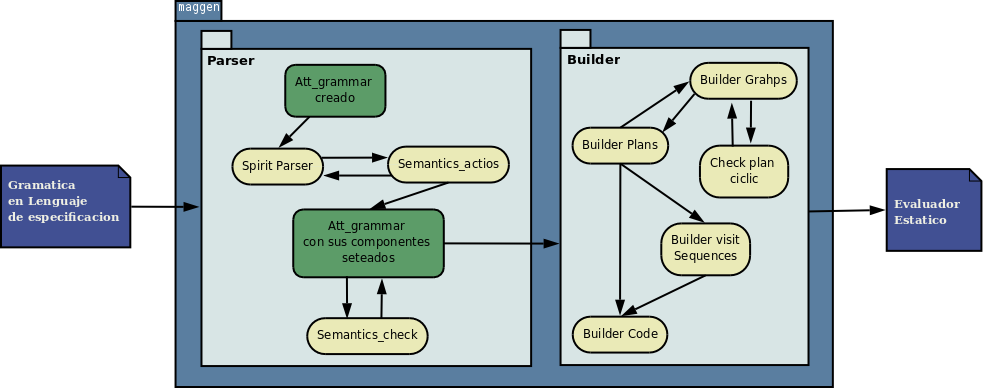
\includegraphics[width=400pt,height=158pt]{Disen.png}
\caption{\label{fig:disen}Interacción de Attr\_grammar en \maggen}
\end{figure}

A continuación se analizan cuestiones de diseño de los paquetes mencionados arriba, y con ellos la estructura \textbtt{Attr\_grammar}.  En la figura \ref{fig:disen2} se muestra un diagrama con la representación interna de una gramática dentro de \maggen.

\begin{figure}[!ht]\centering
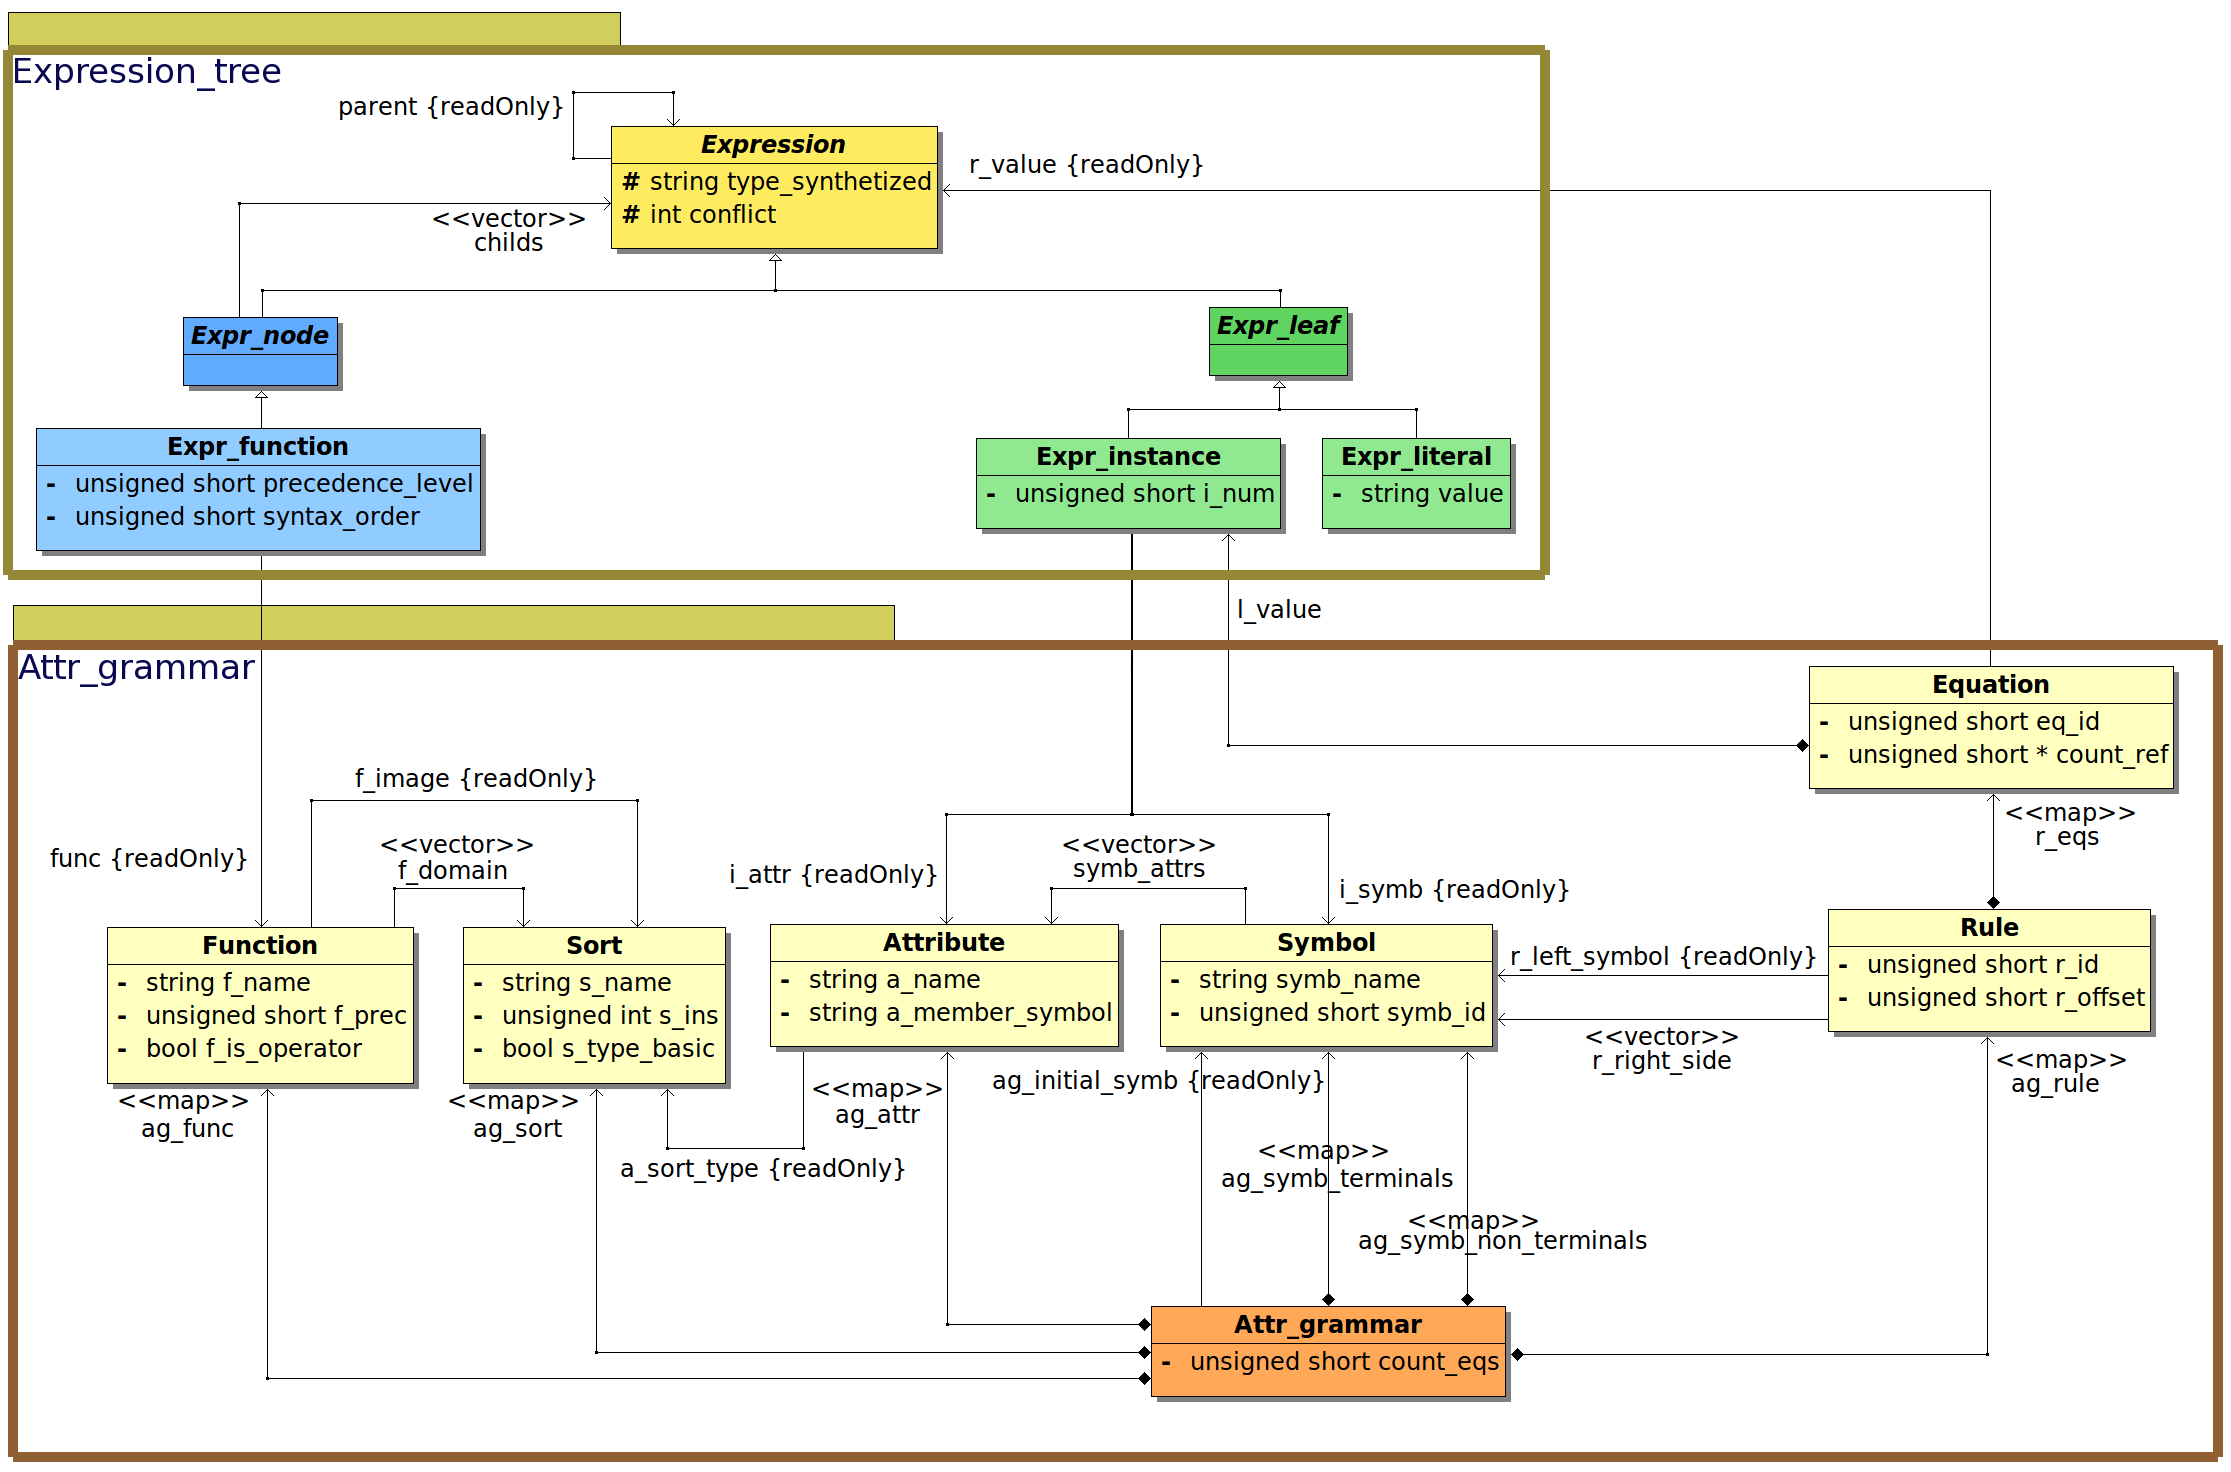
\includegraphics[width=400pt,height=264pt]{Disen2.png}
\caption{\label{fig:disen2}Diseño interno de una gramática de atributos en \maggen}
\end{figure}

Algunas observaciones sobre el diseño realizado en la figura \ref{fig:disen2}:

\begin{itemize}
\item La relación entre los paquetes se produce por un lado, mediante la clase \textbtt{Rule}, en el sentido de que toda regla contiene un conjunto de ecuaciones y cada una de estas, está definida a través de un \textit{l\_value:}\textbtt{Expr\_instance} y un \textit{r\_value:}\textbtt{Expression}. Por otro lado, \textbtt{Expr\_instance} se vincula con \textbtt{Symbol} y \textbtt{Attribute} y \textbtt{Expr\_function} con \textbtt{Function}.

\item Toda la información de una gramática de atributos esta representada en la clase \textbtt{Attr\_grammar} y por ende, el ciclo de vida de cada uno de sus componentes es administrado por esta clase, durante todo el funcionamiento de \maggen. 
\end{itemize}

\subsection{Chequeos}
\label{subsec:check}

El conjuntos de chequeos que se realizan sobre la gramática de entrada a \maggen, están directamente relacionados con el concepto de gramática bien definida analizado en la sección \ref{sec:well-defined}. Además, se aplican una serie de chequeos extras para evitar cálculos inconsistentes en las etapas posteriores. La totalidad de los chequeos, son realizados sobre el bloque de reglas de la gramática\footnote{En su mayoría los chequeos se realizan sobre las ecuaciones de las reglas.}, debido a que este, es el más significativo y sobre el cual se apoyan los cálculos posteriores (en particular, el cálculo de planes).

Los chequeos realizados son clasificados en sintácticos y semánticos, los primeros, en su mayoría, son realizados durante el parser, en cambio, los chequeos semánticos se realizan luego del parser de cada regla, aplicando escaneos específicos. Estos últimos son los explicados en esta sección.

El módulo que agrupa estos chequeos, se ubica en el paquete \textbtt{Parser} de \maggen\ y se denomina \textbtt{Semantics\_checks}.

A continuación se detallan dichos chequeos\footnote{Detalles sobre la implementación de cada uno de los chequeos, ver sección \ref{sec:checksem}}:

\begin{description}
\item [Precedencia] El chequeo de precedencia consiste en preservar la precedencia definida de cada operador. Dicho chequeo, es realizado sobre cada una de las ecuaciones definidas en la gramática. Por ejemplo:\\ Dada la siguiente ecuación:

\begin{center}
 \fbox{\ \textbtt{E[0].valor = E[1].valor + E[2].valor * E[2].valor}\ }
\end{center}

Su interpretación está dada por la definición de la precedencia de los operadores \textbtt{+} y \textbtt{*}(se asume que los dos operadores son infijos y están bien usado). Si se toma \textbtt{*} con mayor precedencia que \textbtt{+}, \maggen\ interpreta implícitamente como si la ecuación tuviera paréntesis:

\begin{center}
 \fbox{\ \textbtt{E[0].valor = E[1].valor + (E[2].valor * E[2].valor)}\ }
\end{center}

El uso de paréntesis en las expresiones define explícitamente la prioridad de los operadores, por lo que, \maggen\ asume esa precedencia. Por ejemplo, si en la ecuación vista arriba se la define utilizando paréntesis, es decir:\  
 \fbox{\ \textbtt{E[0].valor = (E[1].valor + E[2].valor) * E[2].valor}\ }\ la interpretación es tomada en ese sentido.

\item [Asociatividad] El chequeo de asociatividad realiza un análisis sobre las expresiones de las ecuaciones, para asegurar la asociatividad definida de cada operador. Por ejemplo, si se ha definido un operador \textbtt{non\_assoc}, se espera que el uso del mismo sea consistente con esa definición, es decir, no se considere una posible asociación del mismo. 

Cuando se utilizan paréntesis en la expresión, \maggen\ asume la asociatividad que se especifica explícitamente.

\item [Alcanzabilidad] Es una característica importante a tener en cuenta sobre los símbolos de la gramática. Este chequeo, realiza un análisis sobre la totalidad de las reglas en busca de símbolos no terminales no alcanzables desde el símbolo inicial. Este caso no es considerado error fatal en \maggen, sino como \textit{warning}.

\item [Condiciones de AG] Este chequeo tiene en cuenta un conjunto de condiciones que debe cumplir la gramática. Ellos son:

\begin{itemize}
\item Cada regla debe definir todos los atributos sintetizados del símbolo de la parte izquierda.
\item Cada regla debe definir todos los atributos heredados de los símbolos de la parte derecha.
\item Cada regla sólo define los atributos de los símbolos que participan en dicha regla.
\item En caso de redefinición alguna instancia en la regla, la misma es ignorada.
\item Los índices de las instancias deben ser consistentes con la cantidad de apariciones del símbolo en la regla.\\ \underline{\textbf{Ejemplo:}}\\
En la siguiente regla:\ \fbox{\ \textbtt{S ::= S T}\ }\ los índices posibles de las instancias son \textbtt{0} y \textbtt{1} para el símbolo ``\textbtt{S}'' y \textbtt{0} para el símbolo ``\textbtt{T}''.
\item La gramática debe respetar las condiciones exigidas para una gramática extendida. 
\end{itemize}
\end{description}

\section{Construcción de grafos, planes y secuencias de visita}

En la figura \ref{fig:disen} se puede visualizar el funcionamiento de \maggen, teniendo en cuenta la estructura \textbtt{Attr\_grammar}, en esta sección se abordan detalles sobre el diseño del paquete \textbtt{Builder}, específicamente en la construcción de grafos, de planes y de secuencias de visita. Un detalle a tener en cuenta es que, a partir de esta etapa, todas las manipulaciones son realizadas sobre las ecuaciónes de cada regla.

\subsection{Construcción de grafos}
\label{subsec:graph}

Detalles de implementación serán analizados en la sección \ref{subsec:const-graf}, ahora se mencionarán las consideraciones más relevantes con respecto al funcionamiento de los grafos en \maggen.\\

La construcción de grafos se realiza en el módulo \textbtt{builder\_graphs}. \maggen\ crea 4 tipos de grafos, que se corresponden con los detallados en \ref{sec:pre-grafos}:

\begin{itemize}
\item Grafo DP, ver \ref{dpgraph}.
  \begin{figure}[!ht]\centering
    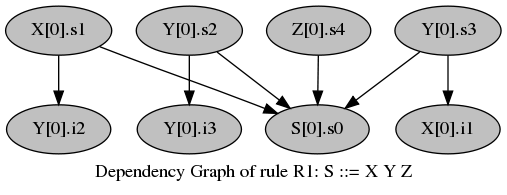
\includegraphics[width=200pt,height=77pt]{graph/dp.png}
  \caption{\label{dpgraph} Grafo DP.}
  \end{figure}

\item Grafo Down, ver \ref{downgraph}.
  \begin{figure}[!ht]\centering
    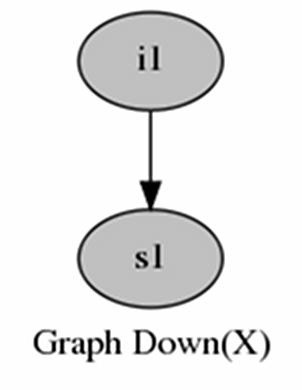
\includegraphics[width=75pt,height=97pt]{graph/down.png}
  \caption{\label{downgraph} Grafo Down.}
  \end{figure}

\item Grafo DCG, ver \ref{dcggraph}.
  \begin{figure}[!ht]\centering
    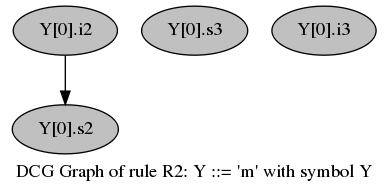
\includegraphics[width=200pt,height=101pt]{graph/dcg.png}
  \caption{\label{dcggraph} Grafo DCG.}
  \end{figure}

\item Grafo ADP, ver \ref{adpgraph}.
  \begin{figure}[!ht]\centering
    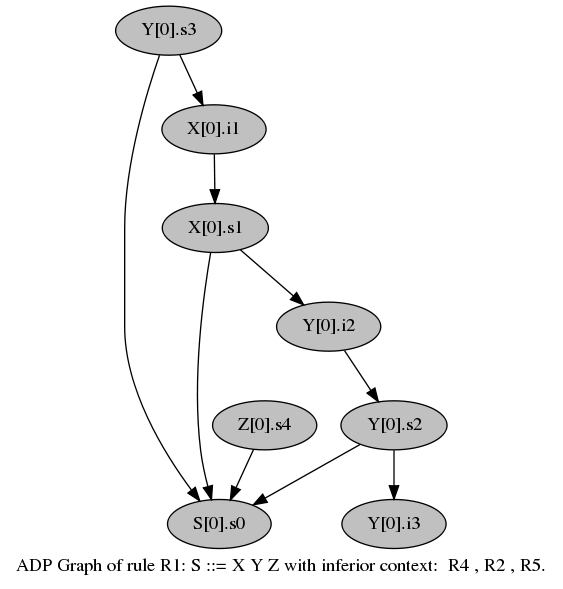
\includegraphics[width=200pt,height=209pt]{graph/adp.png}
  \caption{\label{adpgraph} Grafo ADP.}
  \end{figure}
\end{itemize}

Las figuras\footnote{\label{foot:graph} Imagen generada utilizando la herramienta \textbtt{graphviz} sobre el archivo \textbtt{.dot} generado por \maggen.} muestran un ejemplo de cada tipo de grafo, generadas a partir del ejemplo analizado en el apéndice \ref{append:agwuuyang}.

La construcción de cada tipo de grafo respeta los principios analizados en el capítulo \ref{chap:mag} y los algoritmos respectivo analizados en el capítulo \ref{chap:eval_est}. 

De de los 4 tipos de grafos analizados, los necesarios para el cómputo de etapas siguientes, son los ``\textbtt{ADP graph}''. Los demás, son requeridos como cálculo previo para la construcción de estos.

\subsection{Construcción de planes}
\label{subsec:conts-plan-dise}
La etapa de construcción de planes, tal como lo muestra el diagrama de la figura \ref{fig:disen}, se realiza en el paquete ``\textbtt{Builder}''. El cálculo de planes en \maggen\ se basa en lo analizado en el capítulo \ref{chap:eval_est} (Ver sección \ref{sec:comp-planes}) y teniendo en cuenta estos dos puntos:

\begin{enumerate}
\item El punto de entrada para el cálculo de los planes esta dado sobre los grafos \textbf{ADP}. 
\item El cálculo de planes se basa en un orden topológico de la evaluación de los atributos de los símbolos, teniendo en cuenta los distintos contextos posibles.
\end{enumerate}

En la sección \ref{sec:obtplaneval} se tratan detalles de implementación, en donde se analiza el funcionamiento de lo tratado anteriormente, en especial el punto 2.

Un \textbf{plan} se compone de una lista de números de ecuaciones a computar. Todo plan determina un orden de evaluación, realizándose la evaluación de izquierda a derecha.

\subsubsection{Planes proyectados}

Estos se obtienen a partir de los planes analizados anteriormente, proyectando el plan para cada símbolo de la parte derecha de la regla. La importancia de estos planes radica en la construcción de las secuencias de visita y además en el algoritmo principal de evaluación en la generación de código.

\begin{figure}[!ht]\centering
 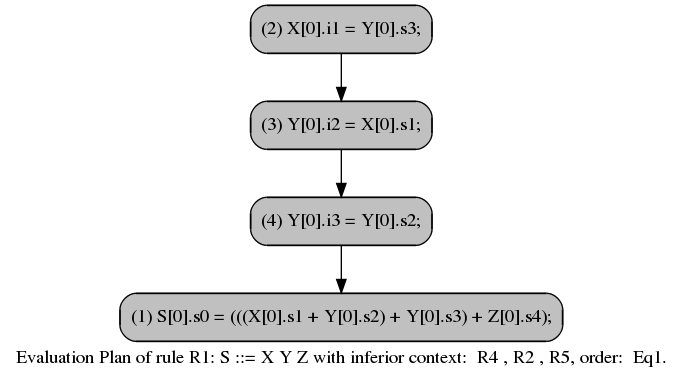
\includegraphics[width=250pt,height=139pt]{plans/plan.png}
\caption{\label{fig:plan}Plan obtenido por \maggen\ para la regla R1}
\end{figure}

En la figura\footnote{Figura obtenida con la herramienta \textbtt{graphviz} sobre el archivo \textbtt{.dot} generado por \maggen.} \ref{fig:plan} se observa un plan obtenido por \maggen\ para el ejemplo del apéndice \ref{append:agwuuyang}. Este plan contiene el orden de los números de ecuación que pertenecen a la regla del plan, los planes proyectados son computados sobre el plan total, es decir con todas las dependencias.

Para clarificar este concepto, se pueden observar los planes proyectados obtenidos en la figura \ref{fig:plan_project}, para el plan de evaluación anterior.

\begin{figure}[!ht]\centering
\begin{tabular}{l l}
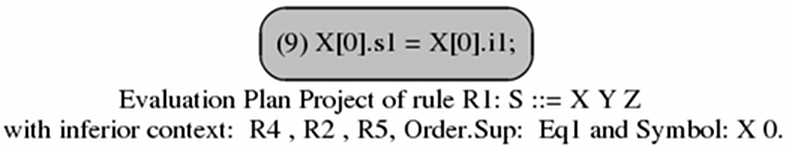
\includegraphics[width=180pt,height=34pt]{plans/plan_proj1.png} &
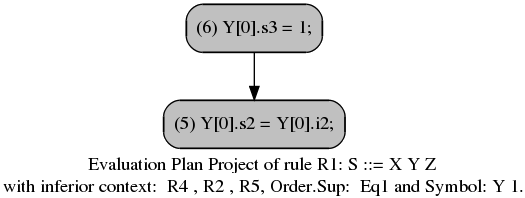
\includegraphics[width=180pt,height=68pt]{plans/plan_proj2.png}\\ 
\multicolumn{2}{c}{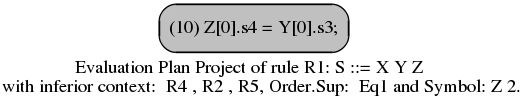
\includegraphics[width=180pt,height=34pt]{plans/plan_proj3.png}}\\
\end{tabular}
\caption{\label{fig:plan_project}Planes proyectados obtenido por \maggen\ para R1.}
\end{figure}

Notar que cada plan proyectado ha capturado las ecuaciones de cada símbolo de la parte derecha para el cómputo de sus atributos, dependiendo del contexto. Es decir, en el caso del símbolo ``\textbtt{Y}'' su orden ha sido computado observando las dependencias de la regla R2. Estas dependencias son necesarias para el cálculo del plan completo en las ecuaciones 2 y 4. 

\subsection{Construcción de secuencias de visita}
\label{sec:constseqvisit}

La etapa de construcción de secuencias de visita, tal como lo muestra el diagrama de la figura \ref{fig:disen}, se realiza en el paquete ``\textbtt{Builder}''. Las mismas, son computados a partir de los diferentes planes obtenidos en el sección anterior.

El funcionamiento para la construcción de las secuencias, esta dado por la aplicación de un recorrido recursivo sobre los contextos de las reglas, para la evaluación de cada atributo de los símbolos. El resultado de este algoritmo, son los valores que conforman la secuencia de visita, tal como se ha analizado en la sección \ref{sec:sec-visit}. Estos valores siguen la siguiente interpretación: 

\begin{description}
\item [Compute] Valor menor que cero que representa el número de la ecuación a resolver\footnote{La ecuación a computar pertenece a la regla del plan corriente.}.
\item [Visit] valor mayor que cero que representa el número nodo hijo a visitar\footnote{El nodo hijo esta dado por el contexto de la regla del plan corriente.}.
\item [Leave] valor ``\textbtt{0}''.
\end{description}

A modo de ejemplo, se muestran las secuencias de visita generadas por \maggen\ para el ejemplo analizado en el apéndice \ref{append:agwuuyang}:

\begin{description}
\item [\{-7,0,-8\}] Secuencia de visita para la regla \textbtt{R3} (sin contexto inferior). En este caso, la secuencia de visita se traduce a lo siguiente:

\begin{enumerate}
\item \textbf{Computar} la ecuación 7.
\item \textbf{Leave}\footnote{El leave retorna el control a la secuencia de visita de contexto superior, es decir, desde donde se invocó a esta secuencia.}.
\item \textbf{Computar} la ecuación 8.
\end{enumerate}

\item [\{-11,1,-12,-10\}] Secuencia de visita para la regla \textbtt{R5} con el contexto de \textbtt{P2}. En este caso, la secuencia de visita se traduce a lo siguiente:

\begin{enumerate}
\item \textbf{Computar} la ecuación 11.
\item \textbf{Visitar} el nodo hijo 1, es decir \textbtt{Y}, como el contexto es \textbtt{P2}, significa visitar a R2.
\item \textbf{Computar} la ecuación 12.
\item \textbf{Computar} la ecuación 10.
\end{enumerate}
\end{description}

Cabe aclarar que todas las secuencias de visita tienen un \textbf{leave} implícito al final, es decir, cuando se completo la computación de la secuencia se retorna a su ámbito de invocación.

\subsubsection{Heurística del algoritmo}
\label{subsec:heuris-simul}
El punto principal en el cual se basa la heurística, es evaluar el plan buscando las dependencias de cada ecuación en el contexto del mismo. A continuación se muestran los pasos básicos a tener en cuenta con un ejemplo:\\

Si se toma uno de los planes\footnote{Es importante notar el hecho de que cada plan se conforma de los números de ecuaciones a computar.} calculados por \maggen\ para el ejemplo del apéndice \ref{append:agwuuyang}:\\

\underline{Plan:} \{ 2, 3, 4, 1 \}. Ver figura \ref{fig:plan}.

\begin{enumerate}
\item Se recorre el plan tomando en cada paso una de las ecuaciones. Para este caso particular se comienza con la ecuación 2.

\item Dada la ecuación \textbtt{i}\footnote{Para este caso particular \textit{i} toma los valores 1,2,3,4.}, en el plan, se debe computar todo el \textit{l\_value} de la ecuación. Para ello se deben resolver todas las dependencias dadas por \textit{r\_value}.

\item Dada una dependencia de la ecuación, primero se chequea si la misma fue computada en algún paso anterior, sino, se analizan los siguientes casos:

\begin{itemize}
\item Si la dependencia proviene de una instancia que pertenece al \textbf{símbolo de la parte izquierda de la regla} y además contiene un \textbf{atributo heredado}, entonces se debe realizar un ``\textbtt{leave}''.

\item Si la dependencia proviene de una instancia que pertenece a un \textbf{símbolo de la parte derecha de la regla} y además contiene un \textbf{atributo sintetizado}, entonces se debe de realizar un ``\textbtt{visit}''. En este caso, se debe analizar, según el contexto, cuál es el plan se debe visitar, es decir, a cuál nodo hijo. 
\end{itemize}

Notar que en los dos puntos anteriores, no se incluyen los casos de dependencia perteneciente al símbolo de la parte izquierda con atributo sintetizado y dependencia de símbolo de la parte derecha con atributo heredado, pero estos casos, son los que deben definirse en este ambiente y como se parte del plan evaluación, el orden de dependencias es consistente con la demanda de las mismas.

\item Luego de la obtención de todas las dependencias, se realiza un \textbf{compute} del \textit{l\_value} y se marca a este como \textbtt{evaluado}. El paso siguiente es avanzar una ecuación en la lista que impone el plan y realizar los mismos tratamientos.
\end{enumerate} 

Para más detalle en la figura \ref{fig:simul} se grafica este proceso.

\begin{figure}[!ht]\centering
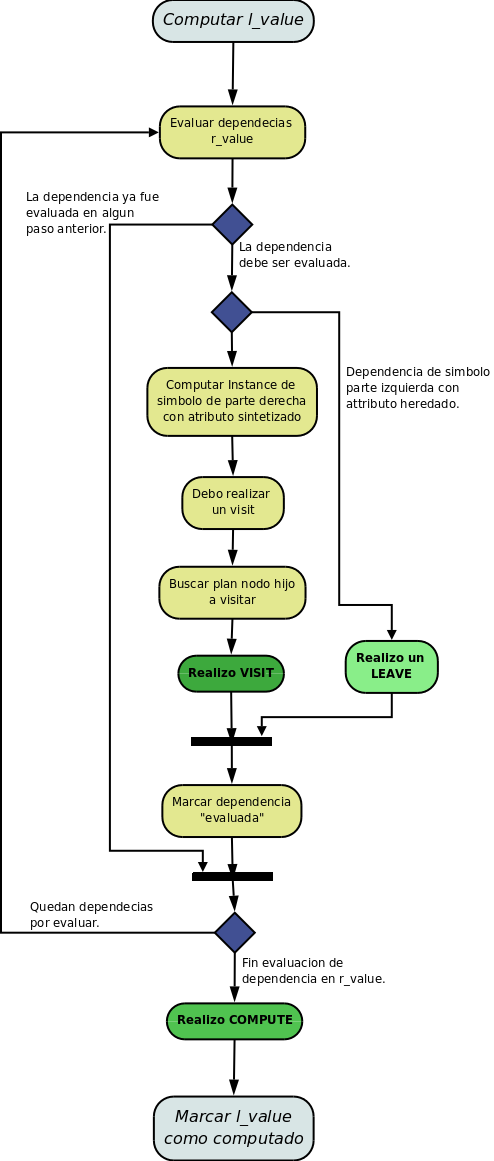
\includegraphics[width=228pt,height=400pt]{simu.png}
\caption{\label{fig:simul}Heurística cómputo de secuencia de visita}
\end{figure}

El resultado del ejemplo, aplicando los pasos tratados arriba, es presentado en el diagrama \ref{fig:resul_vis}.

\begin{figure}[!ht]\centering
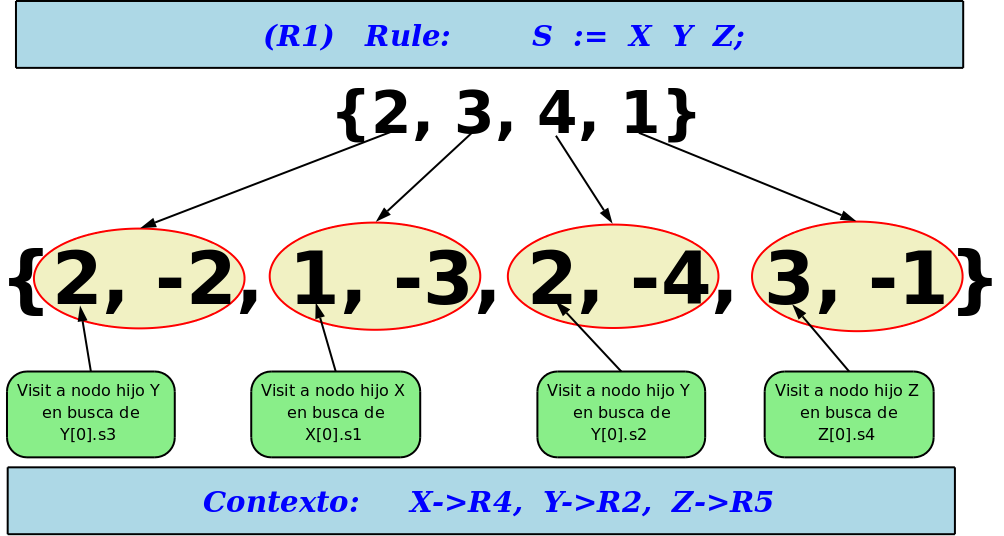
\includegraphics[width=300pt,height=160pt]{plan2seq.png}
\caption{\label{fig:resul_vis} Ejemplo de Secuencia de visita}
\end{figure}

Notar que para el cómputo de las secuencias de visitas totales, solamente basta con lanzar el algortimo, analizado anteriormente, para los planes iniciales\footnote{Los planes iniciales son aquellos que provienen de regla inicial.}. La explicación de esto se sustenta en las propiedades garantizadas con los chequeos en la gramática, principalmente la propiedad de alcanzabilidad. De esta forma, los planes iniciales lanzan los demás planes necesarios para el cómputo total de las secuencias.

\section{Generación de Código}
\label{sec:gencodigo}

La etapa final de \maggen\ esta dada por la generación de código para el evaluador estático. Como se ha analizado en el diagrama visto en la figura \ref{fig:disen}, esta etapa se realiza en el paquete ``Builder'', específicamente en el módulo \textbtt{Builder\_code}.

La etapa de generación de código produce dos archivos: \textit{interface} (.hpp) e \textit{implementación} (.cpp). En el apéndice \ref{append:agwuuyangcode} se puede observar el código generado para el ejemplo de Wuu Yang ya analizado durante todo este capítulo.

A continuación se abordarán algunas consideraciones sobre la generación de código en \maggen\ teniendo en cuenta lo observado en el apéndice.

Consideraciones de la clase:

\begin{description}
\setlength{\itemindent}{1em}
\setlength{\leftmargin}{1em}

\item [Atributos] la totalidad de los mismos tienen visibilidad privada.

\begin{lstlisting}[backgroundcolor=\color{white}, linewidth=9.5cm]
vector <Visit_sequence> v_seq;
vector <Order_rule>     contexts_rule;
vector <Plan>           eval_plans;
vector <Plan_project>   eval_plans_project;
vector <Rule>           rules;
\end{lstlisting}

Estos, son usados por los métodos del evaluador generado por \maggen. Se puede hacer una diferencia en el hecho de que, \textbtt{v\_seq} es usado directamente por el algoritmo de evaluación, en cambio los demás son usados por algoritmos previos a este. Cada uno de los tipos usados para estos atributos son definidos en otro módulo, el cual se analizará más adelante.

\item [Métodos] Es necesario distinguirlos según su visibilidad:

\begin{itemize}
\setlength{\itemindent}{1em}
\setlength{\leftmargin}{1em}
\item Privados:

\begin{lstlisting}[backgroundcolor=\color{white}, columns=fullflexible]
void add_plan(const Key_plan &k_plan, unsigned short index_order);
void add_plan_project(const Key_plan_project &k_plan_p, unsigned short index_order);
void compute_eq(int num_eq, struct Node *root);
void traverse(struct Node *node, unsigned short order);
void eval_visiter(struct Node *root);
\end{lstlisting}

Estos métodos son usados internamente por el evaluador generado por \maggen\ teniendo en cuenta lo siguiente:\\
\textbtt{compute\_eq} tiene la responsabilidad de invocar a los \textbf{compute} de cada ecuación y \textbtt{eval\_visiter} tiene la responsabilidad de los \textbf{visit} a nodos. Notar que, estos métodos trabajan sobre las secuencias de visita.

El método \textbtt{traverse} recorre el AST de entrada al evaluador y asigna a cada nodo un plan de evaluación\footnote{Los planes que asigna el método traverse son los generados estáticamente por \maggen.} y con ello una secuencia de visita correspondiente.

\textbtt{add\_plan} y \textbtt{add\_plan\_project} agregan planes y planes proyectados respectivamente, los mismos son usados en la inicialización del evaluador (constructor de clase).

\item Públicos:

\begin{lstlisting}[backgroundcolor=\color{white}, columns=fullflexible, linewidth=7cm]
maggen();
void print_visit_seqs();
void translates_visit_seqs();
void evaluator_mag(struct Node *root);
\end{lstlisting}

Estos, son los servicios públicos que ofrece el evaluador generado por \maggen. El método más importante, es \textbtt{evaluator\_mag}, el cual pone en funcionamiento el evaluador generado por \maggen. El parámetro tomado por el método representa la raíz del AST que se desea evaluar.

El constructor de clase\footnote{El nombre de la clase y por ende el del constructor de la misma depende de los parámetros con los cuales se invocó a \maggen\ (Ver capítulo \ref{chap:usos}).} realiza la inicialización de los atributos de la misma. Los valores de inicialización de los atributos son obtenidos por los cómputos de cada etapa de \maggen\ vistas en todo este capítulo.

Los dos métodos anexos, \textbtt{print\_visit\_seqs} y \textbtt{translates\_visit\_seqs} pueden ser usados para visualizar las secuencias de visita del evaluador. Los dos realizan la misma funcionalidad, pero muestran las secuencias de visita de manera diferente, como lista de valores o como secuencia de \textbtt{compute}, \textbtt{visit} o \textbtt{leave}.
\end{itemize}
\end{description}

Además de la clase, \maggen\ genera \textbtt{struct} para cada uno de los símbolos de la gramática y para cada uno implementa el método \textbtt{to\_string()} que se responsabiliza de como mostrar por pantalla cada símbolo, teniendo en cuenta sus atributos. Para más detalles analizar en el apéndice \ref{append:agwuuyangcode}, específicamente los \textbtt{struct} para los símbolos \textbtt{S, X, Y, Z}.

Los dos módulos analizados arriba, generados por \maggen, se apoyan sobre dos módulos más, que son anexados de manera estática por la herramienta, ellos son: \textbtt{Node.hpp} y \textbtt{Plan.hpp}.

Los mismos contienen definiciones de ``tipos'' y ``métodos'' necesarios por el el evaluador generado.

\subsection{Cabecera: \textbtt{Node.hpp}}

El tipo de datos nodo de un AST, se encuentra definido en este archivo. Los campos del mismo son:
\begin{items}
\item \textbtt{struct Node *parent:} referencia al nodo superior.

\item \textbtt{vector <struct Node*>\ childs:} listado de referencias a los hijos.

\item \textbtt{unsigned short rule\_id:} identificador de la regla que representa el nodo.

\item \textbtt{unsigned short visit\_seq\_index:} índice de la secuencia de visita que le corresponde al nodo para su evaluación.

\item \textbtt{unsigned short pos\_visit\_seq:} posición desde donde debe comenzar a recorrerse la secuencia de visita.
\end{items}

Además se encuentra su constructor y una funcionalidad para agregar hijos.

\subsection{Cabecera: \textbtt{Plan.hpp}}

Aquí se encuentran las definiciones de tipos necesarios para el evaluador:

\begin{items}
\item Orden de evaluación de ecuaciones:
\begin{lstlisting}[backgroundcolor=\color{white}, columns=fullflexible, linewidth=11.5cm]
typedef vector <unsigned short> Order_eval_eq;
\end{lstlisting}

\item Orden de evaluación de reglas (contexto):
\begin{lstlisting}[backgroundcolor=\color{white}, columns=fullflexible, linewidth=11.5cm]
typedef vector <unsigned short> Order_rule;
\end{lstlisting}

\item Clave para planes de evaluación:
\begin{lstlisting}[backgroundcolor=\color{white}, columns=fullflexible, linewidth=11.5cm]
typedef struct k_plan
{
    unsigned short  id_plan;
    unsigned short  plan;
    ...
} Key_plan;
\end{lstlisting}

\item Clave para planes de evaluación proyectados:
\begin{lstlisting}[backgroundcolor=\color{white}, columns=fullflexible, linewidth=11.5cm]
typedef struct k_p_project
{
    Key_plan        id_plan_project;
    unsigned short  node_project;
    unsigned short  index_ocurrence;
    ...
} Key_plan_project;
\end{lstlisting}

\item Secuencia de visita:
\begin{lstlisting}[backgroundcolor=\color{white}, columns=fullflexible, linewidth=11.5cm]
typedef vector <int> Visit_sequence;
\end{lstlisting}

\item Versión reducida de regla:
\begin{lstlisting}[backgroundcolor=\color{white}, columns=fullflexible, linewidth=11.5cm]
typedef vector <unsigned short> Rule;
\end{lstlisting}

\item Plan de evaluación:
\begin{lstlisting}[backgroundcolor=\color{white}, columns=fullflexible, linewidth=11.5cm]
typedef pair <Key_plan, unsigned short> Plan;
\end{lstlisting}

\item Plan de evaluación proyectado:
\begin{lstlisting}[backgroundcolor=\color{white}, columns=fullflexible, linewidth=11.5cm]
typedef pair <Key_plan_project, unsigned short> Plan_project;
\end{lstlisting}
\end{items}

\normalsize
       % Diseño de magGen.
1\chapter{Detalles de Implementación de \maggen}
\label{chap:implem}
\minitoc

En esta sección se aclararan y expondrán decisiones que se realizaron a lo largo de la implementación de esta herramienta.

Primero, como ya se menciona en el capítulo anterior, el lenguaje sobre el cual se realizó el desarrollo de \maggen\ es C++, con lo que todo el código es principalmente característico de un modelo de programación Orientado a Objetos, aunque posee secciones de Programación Imperativa, para lograr ciertas optimizaciones y poder integrar componentes de externos a la herramienta.

\section{Parsing usando \boost\ \spirit}

El primer desafío de codificación, fue que se debía conseguir parsear el archivo de entrada de la herramienta, en el cual vendría la especificación de una Gramática de Atributos, respetando la sintaxis presentada anteriormente, o no.

La solución obtenida se apoya en la utilización de un framework reconocido mundialmente, denominado \spirit, perteneciente a la biblioteca de C++ llamada \boost. Esta decisión trajo dos grandes beneficios; la confiabilidad de el parser obtenido y la rápida obtención del mismo, ya que la gran ventaja de \spirit, es que permite escribir la definición de la gramática en lenguaje \textbf{C++}.

\spirit\ es un framework generador de analizadores sintácticos, o parsers, descendentes recursivos orientado a objetos implementado usando técnicas de meta-programación con plantillas. Las expresiones mediante plantillas, permiten aproximar la sintaxis de una ``\textit{\textit{Forma Backus Normal Extendida}}'' (\textbf{EBNF}) completamente en C++.

Se puede resumir que el proceso de análisis sintáctico, en este framework, se componente de cuatro partes.

\begin{figure}\centering
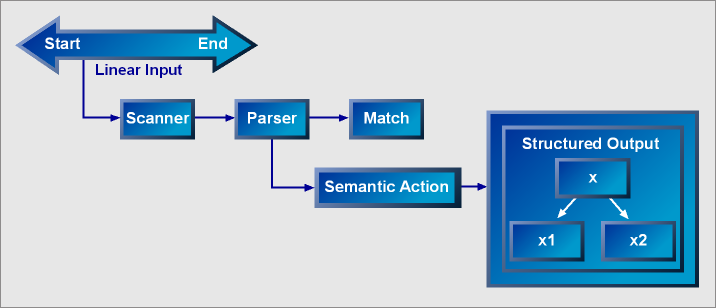
\includegraphics[width=450pt, height=180pt]{./spirit.png}
\caption{Procesos dentro de \spirit}\label{procesoSpirit}
\end{figure}

El usuario es el responsable de definir las ``\texttt{semantic actions}'' para lograr capturar los resultados intermedios, producidos durante la etapa de parsing y no sólo obtener un valor lógico sobre si se pudo o no, consumir toda la cadena de entrada.

Para comenzar a definir una gramática hay que crear una estructura que herede de la clase \texttt{grammar}. Dentro de ella se debe definir a su vez otra estructura templatizada denominada \texttt{definition}. En donde realmente estará la definición de la gramática.

\begin{lstlisting}[language=C++, basicstyle=\scriptsize,numbers=left, numbersep=5pt, numberstyle=\tiny]
struct my_grammar: public grammar <my_grammar>
{
    template <typename ScannerT>
    struct definition
    {
        rule <ScannerT> r;

        definition(my_grammar const& self)
        {
            r = /*... Aqui va la definicion ...*/;
        }
        rule <ScannerT> const& start() const
        {
            return r;
        }
    };
};
\end{lstlisting}

Para definirla, disponemos de un amplio conjunto de herramientas. Primero, los operadores de metalenguaje listados en la tabla \ref{ope_spirit}, los cuales permiten construir nuevas reglas combinando reglas ya definidas, parsers y constantes permitidas en el framework.

\begin{figure}\centering\scriptsize
\begin{tabular}{| c | p{7cm} |}
\hline
\multicolumn{1}{|>{\columncolor[rgb]{0.8, 0.8, 0.8}}l|}{\textbf{Operador}} &
\multicolumn{1}{|>{\columncolor[rgb]{0.8, 0.8, 0.8}}l|}{\textbf{Semántica}} \\ \hline
A $=$                  B  & Definición de A en base a B \\ \hline
A $|$                  B  & Unión, acepta A o B, también llamada ``alternativa''\\ \hline
A $\&$                 B  & Intersección, acepta A y B \\ \hline
A $-$                  B  & Diferencia, acepta A pero no a B  \\ \hline
A $\textasciicircum$   B  & Disyunción exclusiva, acepta A o B, pero no a ambos \\ \hline
A $>>$                 B  & Secuencia, acepta A seguido de B \\ \hline
\multirow{2}{*}{A $\%$ B} & Lista, acepta A separados por ocurrencias de B.\\
                          & Es equivalente a: A $>>$ *(B $>n$ A)\\ \hline
$*$                    A  & Estrella de Kleene, 0 o más veces \\ \hline
$+$                    A  & Positivo, 1 o más veces \\ \hline
$!$                    A  & Opcional, 0 o 1 vez \\ \hline
\end{tabular}
\caption{Operadores de \spirit\ utilizados}\label{ope_spirit}
\end{figure}

Por otra parte, \spirit\ dispone de un gran conjunto de parsers que abarcan la mayoría de los tipos básicos, representación de datos y valores utilizados en el común de los lenguajes (ver tabla \ref{parsers}).

\begin{figure}\centering\scriptsize
\begin{tabular}{| l | l |}
\hline
\multicolumn{1}{|>{\columncolor[rgb]{0.8, 0.8, 0.8}}l|}{\textbf{Parser}} &
\multicolumn{1}{|>{\columncolor[rgb]{0.8, 0.8, 0.8}}l|}{\textbf{Entrada aceptada}} \\ \hline
anychar\_p & Cualquier carácter simple (incluyendo el carácter nulo: '$\setminus0$')\\ \hline
alnum\_p   & Caracteres alfa-numéricos \\ \hline
alpha\_p   & Caracteres alfabéticos \\ \hline
% blank\_p & Un espacio o tabulación \\ \hline
digit\_p   & Dígitos numéricos \\ \hline
lower\_p   & Caracteres en minúscula \\ \hline
upper\_p   & Caracteres en mayúscula \\ \hline
space\_p   & Espacios, tabulaciones, saltos de línea y nuevas líneas \\ \hline
ch\_p      & Carácter especificado como parámetro \\ \hline
str\_p     & Cadena especificada como parámetro \\ \hline
oct\_p     & Dígito en octal \\ \hline
hex\_p     & Dígito en hexadecimal \\ \hline
uint\_p    & Número entero sin signo de 32 bits\\ \hline
int\_p     & Número entero 32 bits\\ \hline
real\_p    & Número flotante 32 bits\\ \hline
eps\_p     & Cadena vacía (épsilon)\\ \hline
end\_p     & Carácter de fin de archivo (EOF)\\ \hline
\end{tabular}
\caption{\label{parsers} Parsers predefinidos de \spirit\ utilizados} 
\end{figure}

Además posee varias directivas que modifican el comportamiento de los parsers, encapsulándose en una expresión definida por el usuario (ver tabla \ref{directivas}).

\begin{figure}\centering\scriptsize
\begin{tabular}{| l | p{7cm} |}
\hline
\multicolumn{1}{|>{\columncolor[rgb]{0.8, 0.8, 0.8}}l|}{\textbf{Directiva}} &
\multicolumn{1}{|>{\columncolor[rgb]{0.8, 0.8, 0.8}}l|}{\textbf{Efecto}} \\ \hline
lexeme\_d    & Deshabilita la omisión de espacios en blanco (space\_p)\\ \hline
as\_lower\_d & Convierte en minúscula lo aceptado por la expresión\\ \hline
\multirow{3}{*}{longest\_d} & Deshabilita el corto circuito, manda al analizador que\\
                            & pruebe todas las alternativas posibles y elija la secuen-\\
                            & cia más larga aceptada \\ \hline
\end{tabular}
\caption{\label{directivas} Directivas de \spirit\ aplicadas}
\end{figure}

Para el manejo de los símbolos válidos dentro de la definición de la gramática, \spirit\ soporta nativamente, el concepto de ``Tablas de símbolos''. Lo que permite registrar de manera dinámica nuevos símbolos, en particular dentro de nuestra herramienta nos ayudó a manejar los conjuntos de nombres válidos para los \texttt{sorts}, los símbolos no terminales permitidos en las ecuaciones, entre otros usos.

Para comenzar a interactuar con el framework, el usuario debe declarar un objeto de la estructura definida y pasarlo como parámetro a una función específica de \spirit.

\begin{lstlisting}[language=C++, basicstyle=\scriptsize, numbers=left, numbersep=5pt, numberstyle=\tiny]
my_grammar g;

if (parse(first, last, g, space_p).full)
{
    cout << "Parsing Succeeded\n";
}
else
{
    cout << "Parsing Failed\n";
}
\end{lstlisting}

\section{Gramática de Atributos con \spirit}

Lo primero que se tuvo que realizar, fue definir los componentes básicos que se iban a necesitar para construir las demás declaraciones.

\begin{description}
\item [Identificadores] son los nombres de sorts, funciones, atributos, símbolos no terminales y reglas, permitidos por \maggen\ y se basan en el común de los estándares. Debido a que el lenguaje del evaluador generado es C++, todas las palabras reservadas de ese lenguaje, son de la misma clase para nuestra herramienta.

\begin{lstlisting}[language=C++, basicstyle=\scriptsize, numbers=left, numbersep=5pt, numberstyle=\tiny]
r_ident = lexeme_d[(alpha_p|'_')>>*(alnum_p|'_')]-r_reserved_word;

r_reserved_word = str_p("compute")|"end"
                | "all"
                | "semantic domain"|"attributes" |"rules"
                | "sort"|"op"|"function"
                | "infix"|"prefix"|"postfix"
                | "syn"|"inh"
                | "left"|"right"|"non-assoc"
                | r_cpp_reserved_words;

r_cpp_reserved_words = r_cpp_basic_types
                     | str_p("and")|"and_eq"|"asm"|"auto"|"bitand"
                     | "bitor"|"break"|"case"|"catch"|"class"|"compl"
                     | "const"|"const_cast"|"continue"|"default"
                     | "delete"|"do"|"double"|"dynamic_cast"|"else"
                     | "enum"|"explicit"|"export"|"extern"|"false"
                     | "for"|"friend"|"goto"|"if"|"inline"|"long"
                     | "mutable"|"namespace"|"new"|"not"|"not_eq"
                     | "operator"|"or"|"or_eq"|"private"|"protected"
                     | "public"|"register"|"reinterpret_cast"|"return"
                     | "short"|"signed"|"sizeof"|"static"|"static_cast"
                     | "struct"|"switch"|"template"|"this"|"throw"|"true"
                     | "try"|"typedef"|"typeid"|"typename"|"union"
                     | "unsigned"|"using"|"virtual"|"void"|"volatile"
                     | "wchar_t"|"while"|"xor"|"xor_eq";

r_cpp_basic_types = str_p("bool")|"char"|"float"|"int"|"string";
\end{lstlisting}

\item [Operadores] Dentro de la especificación de la GA, se permiten como nombre válidos para los operadores, caracteres alfabéticos, numéricos y los operadores básicos de C++. 

\begin{lstlisting}[language=C++, basicstyle=\scriptsize, numbers=left, numbersep=5pt, numberstyle=\tiny]
r_oper = lexeme_d[(alpha_p|'_'|r_id_op)>>*(alnum_p|'_'|r_id_op)];

r_id_op = ch_p('+')|'*'|'/'|'^'|'%'|'&'|'<'|'='|'-'|'>'|'|'|'~'|'.'|','|'?';
\end{lstlisting}

\item [Literales] Son los valores de constantes y tipos básicos aceptados, se adecuan a los estándares de C++. Solamente se tuvo que definir los valores lógicos, los caracteres entre comillas simples y las cadenas de caracteres entre comillas dobles, ya que para los tipos numéricos, existen parsers predefinidos de \spirit\ como ya se dio a conocer.

\begin{lstlisting}[language=C++, basicstyle=\scriptsize, numbers=left, numbersep=5pt, numberstyle=\tiny]
r_boolean = str_p("true")|"false";

r_char = lexeme_d[ch_p('\'')>>(anychar_p)n>ch_p('\'')];

r_string = lexeme_d[ch_p('\"')>>r_string_lit>>ch_p('\"')];

r_string_lit = +((anychar_p-(ch_p('\"')|"\\"|'\'' ))|r_esc_seq);

r_esc_seq = ch_p('\\')>>
            ( oct_p
            | as_lower_d['x']>>hex_p
            | (anychar_p-ch_p('\n'))
            );               
\end{lstlisting}
\end{description}

Para tener una consistencia de identificadores para cada componente de la gramática, utilizamos tablas de símbolos como repositorio, pero también como regla para limitar los posibles valores en posteriores definiciones.

\begin{lstlisting}[language=C++, basicstyle=\scriptsize,numbers=left, numbersep=5pt, numberstyle=\tiny]
symbols <> st_sorts;
symbols <> st_op_prefix;
symbols <> st_op_infix;
symbols <> st_op_postfix;
symbols <> st_functions;
symbols <> st_attributes;
symbols <> st_non_terminal;
\end{lstlisting}

\subsection{\texttt{``semantic domain''} en \spirit}

En esta sección de la especificación se debían aceptar tres tipos de elementos: \texttt{sorts}, \texttt{operators} y \texttt{functions}.

Los \texttt{sorts} serán los tipos que se podrán utilizar para definir los dominios e imágenes de los operadores y funciones.

Según lo explicado en el Diseño, las reglas de cada clase, han sido codificados de la siguiente manera.

\begin{description}
\item [\texttt{sorts}] Exigimos que luego del identificador ``\texttt{sort}'' halla un espacio\footnote{\label{foot:espacio} Ver definición de \texttt{space\_p} \ref{parsers}}. El nombre leído, se usará para crear un nuevo Sort dentro de la GA y también se insertará en la tabla de símbolos de sorts. Se acepta una lista de nombres de sorts para comodidad del usuario.

\begin{lstlisting}[language=C++, basicstyle=\scriptsize, numbers=left, numbersep=5pt, numberstyle=\tiny]
r_decl_sort = lexeme_d[str_p("sort")>>space_p]>>
              (r_ident[&create_sort][st_sorts.add]%',')>>
              ';';
\end{lstlisting}

\item [\texttt{operators}] Para los operadores también se exige el espacio$^{\ref{foot:espacio}}$ luego de la cadena ``\texttt{op}''. Por definición se aceptan tres tipos: infijos, prefijos y posfijos, por lo que se hizo una regla para cada uno, solamente discriminado los dominios, ya que todos poseen una sóla imagen. Notar que los sorts permitidos, son sacados directamente de las tablas de símbolos destinadas para ese propósito.

\begin{lstlisting}[language=C++, basicstyle=\scriptsize, numbers=left, numbersep=5pt, numberstyle=\tiny]
r_decl_oper  = lexeme_d[str_p("op")>>space_p][&inic_func]>>
               (r_oper_infix|r_oper_postfix|r_oper_prefix)>>
               str_p("->")>>
               r_sort_st[&save_image_func]>>
               ';';

r_oper_infix = str_p("infix")[&save_mode_op]>>
               !r_oper_mode>>
               r_oper[&save_name_func][st_op_infix.add]>>
               ':'>>
               r_sort_st[&save_domain_func]>>','>>r_sort_st[&save_domain_func];

r_oper_postfix = str_p("postfix")[&save_mode_op]>>
                 !r_oper_mode>>
                 r_oper[&save_name_func][st_op_postfix.add]>>
                 ':'>>
                 r_sort_st[&save_domain_func];

r_oper_prefix = !(str_p("prefix")[&save_mode_op])>>
                !r_oper_mode>>
                r_oper[&save_name_func][st_op_prefix.add]>>
                ':'>>
                r_sort_st[&save_domain_func];

r_oper_mode = '('>>
               (uint_p[&save_prec_op]|'_')>>
               ','>>
               (r_oper_assoc[&save_assoc_op]|'_')>>
               ')';

r_oper_assoc = str_p("left")|"right"|"non-assoc";
\end{lstlisting}

\item [\texttt{functions}] Para las funciones se permiten como dominio listas de sorts, los cuales serán agregados incrementalmente a la función que se está declarando. La utilización de acciones semánticas facilitan la modularización. La declaración comienza con la cadena ``\texttt{function}'' seguida de una espacio$^{\ref{foot:espacio}}$.

\begin{lstlisting}[language=C++, basicstyle=\scriptsize, numbers=left, numbersep=5pt, numberstyle=\tiny]
r_decl_func = lexeme_d[str_p("function")>>space_p]>>
              r_oper[&inic_func][&save_name_func][st_functions.add]>>
              ':'>>
              !r_dom_func>>
              str_p("->")>>
              r_sort_st[&save_image_func]>>
              ';';

r_dom_func = r_sort_st[&save_domain_func]%',';
\end{lstlisting}
\end{description}

\subsection{\texttt{``attributes''} en \spirit }

Para la codificación de esta sección la funcionalidad buscada era que el usuario mediante una expresión en términos de conjuntos definiera la pertenencia de cada atributo. Por lo que se tuvo que implementar un ``mini-intérprete'' sobre expresiones de conjuntos.

Un detalle a tener en cuenta, en este punto, es que no se encuentra declarado ningún símbolo no terminal'', así que todo símbolo mencionado dentro de la expresión será creado bajo demanda.

La vinculación de los atributos con sus respectivos dueños, se realizará más adelante, debido a que existe la posibilidad de declarar un atributo para todo símbolo, mediante la sentencia \texttt{all}, antes de tener totalmente definido el conjunto de símbolos no terminales de la gramática.

\begin{lstlisting}[language=C++, basicstyle=\scriptsize, numbers=left, numbersep=5pt, numberstyle=\tiny]
r_attributes = lexeme_d[str_p("attributes")>>space_p]>>
               +r_decl_attr[&create_attributes];

r_decl_attr = (r_ident[&add_attribute][st_attributes.add]%',')>>
              ':'>>
              !(r_type_attr[&save_type_attr])>>
              '<'>>r_sort_st[&save_sort_attr]>>'>'>>
              lexeme_d[str_p("of")>>space_p]>>
              (r_conj_symb |
               (str_p("all")n>!('-'>>r_conj_symb))
              )[&save_member_list_attr]>>
              ';';

r_conj_symb = '{'>>(r_ident%',')>>'}';

r_type_attr = str_p("inh")|"syn";
\end{lstlisting}

\subsection{\texttt{``rules''} en \spirit}

En la definición de una gramática las reglas son los pilares, por eso en esta sección se debía brindar la mayor flexibilidad al usuario.

El bloque de reglas comienza con el identificador ``\texttt{rules}'', seguida de un espacio$^{\ref{foot:espacio}}$ y una lista de reglas. Cada una de las mismas son enumeradas desde 1 para mantener una indexación interna. Una vez consumido el bloque se realizan los chequeos que determinan si la GA es MAG o no.

\begin{lstlisting}[language=C++, basicstyle=\scriptsize, numbers=left, numbersep=5pt, numberstyle=\tiny]
r_rules = lexeme_d[str_p("rules")>>space_p]>>
          (+r_decl_rule)>>eps_p[&check_well_defined];
\end{lstlisting}

Una regla individualmente esta representada por un identificador y los caracteres ``\texttt{::=}'' y una lista de símbolos, dejando también la posibilidad de escribir reglas abreviadas mediante el uso del operador ``|'' junto a una nueva lista de símbolos, evitando repetir el lado izquierdo de la regla.

\begin{lstlisting}[language=C++, basicstyle=\scriptsize, numbers=left, numbersep=5pt, numberstyle=\tiny]
r_decl_rule = r_ident[&create_new_non_terminal][&create_rule][st_non_terminal.add]>>
              str_p("::=")>>
              r_right_rule[&save_rule]>>
              *(str_p("|")[&create_abbreviated_rule]>>
              r_right_rule[&save_rule])>>
              ';';
\end{lstlisting}

Dentro de la lista de símbolos se aceptan identificadores de símbolos no terminales y símbolos terminales, definidos mediante una regla específica. Ambos, son creados controlando que no existan repetidos, actualizando la tabla de símbolos solamente de los no terminales.

Se consideran símbolos terminales a cualquier cadena de caracteres encerrada entre comillas simples.

Por definición, una regla puede no contener un bloque de ecuaciones, por lo que es opcional.

\begin{lstlisting}[language=C++, basicstyle=\scriptsize, numbers=left, numbersep=5pt, numberstyle=\tiny]
r_right_rule = +( r_ident[&create_new_non_terminal][st_non_terminal.add]
                | r_terminal[&create_new_terminal]
                )[&save_right_side_rule]>>
               !r_compute_eq;

r_terminal = lexeme_d[ch_p('\'')>>r_string_lit>>ch_p('\'')];
\end{lstlisting}

El mismo estará delimitado por las cadenas \texttt{``compute}'' y \texttt{``end}'', en su interior se aceptará una lista con al menos \textbf{una} ecuación.

Dentro de la definición sólo se podrán utilizar instancias de atributos de los símbolos no terminales que aparecen en la declaración de la regla. Además se debe especificar el índice de ocurrencia, el cual debe cumplir las siguientes condiciones:

\begin{enumerate}
\item Debe ser positivo.
\item El símbolo de la izquierda de la regla tiene el índice 0.
\item Los símbolos no terminales de la parte derecha de la regla, están numerados de izquierda a derecha arrancando en 0 para cada símbolo diferente.
\end{enumerate}

Cada ecuación tiene una instancia de atributo, como ``\texttt{l-value}'', el carácter ``\texttt{=}'' y una expresión como ``\texttt{r-value}''.

\begin{lstlisting}[language=C++, basicstyle=\scriptsize, numbers=left, numbersep=5pt, numberstyle=\tiny]
r_compute_eq = lexeme_d[str_p("compute")>>space_p]>>
               +(r_equation)>>
               str_p("end");

r_equation = r_instance[&create_equation]n>
             '='>>
             r_expression[&save_rvalue]>>
             ';';
\end{lstlisting}

La herramienta acepta cualquier tipo de expresión, ya que se permite que se definan nuevos operadores y funciones según las necesidades de la gramática para la cual se generará el evaluador. Se utilizó la gramática de expresiones ambiguas que figura en la mayoría de los libros de análisis de lenguajes.

\begin{lstlisting}[backgroundcolor=\color{white}]
E := E op E
   | (E)
   | literal
\end{lstlisting}

Donde ``op'' se interpreta como cualquier operador. Esta gramática presentaba el problema de la ``recursión a izquierda'', por lo que se la quitó obteniendo lo siguiente.

\begin{lstlisting}[backgroundcolor=\color{white}]
E := T op1 E
   | T

T := F op2 T
   | F

F := (E)
   | literal
\end{lstlisting}

En nuestra especificación, los ``literales'' pueden ser solamente de tres tipos: funciones, instancias de atributos y los literales propiamente dichos (caracteres, cadenas, valores lógicos, números enteros y flotantes). Los operadores fueron discriminados puntualmente según su sintaxis.

Además, debido a una restricción de \spirit, se tuvo que reescribir toda regla de la forma:

\begin{center}\textbf{\large{$A\ :=\ B\ A\ |\ B\ \ \ \ \Rightarrow\ \ \ \ A\ :=\ B\ (A)*$}}\end{center}

Logrando la siguiente gramática de expresiones, que luego fue codificada en \spirit.

\begin{lstlisting}[backgroundcolor=\color{white}]
E := T (op_infix E)*

T := F (op_postfix)*
   | op_prefix T

F := (E)
   | function
   | literal
   | instance

literal := real
         | int
         | char
         | string
         | bool
\end{lstlisting}

Dentro de las expresiones se tenía que ir resolviendo la precedencia de los operadores declarados por el usuario. Además, la utilización de paréntesis crea distintos niveles de precedencia. Cada vez que se utiliza la producción que genera \texttt{( E )}, la precedencia de los operadores que se utilicen en la expresión \texttt{E}, se resolverán en ese nivel.

\begin{lstlisting}[language=C++, basicstyle=\scriptsize, numbers=left, numbersep=5pt, numberstyle=\tiny]
r_expression = r_expr_prime>>*(r_op_infix_st[&create_operator][&create_func_node]>>
               r_expr_prime[&create_root_infix_node]);

r_expr_prime = r_expr_prime_prime>>
               *(r_op_postfix_st[&create_operator][&create_func_node]
                                [&create_root_postfix_node])
             | r_op_prefix_st[&create_operator][&create_func_node]>>
               r_expr_prime[&create_root_prefix_node];

r_expr_prime_prime = ch_p('(')[&increment_level]>>
                        r_expression>>
                     ch_p(')')[&decrement_level]
                   | r_function[&create_root_function_node]
                   | r_literal[&create_literal_node]
                   | r_instance[&create_instance_node];
\end{lstlisting}

Las definiciones de los tres tipos de literales son coherentes con el estilo de codificación que se usó hasta el momento.

Las funciones aceptan expresiones como parámetros, así que, la asociatividad y precedencia de esas expresiones se resuelve entre los paréntesis explícitos que se exigen en la invocación a una función.

Al completar esta regla se creará una \texttt{Expr\_function} dentro de la gramática.

\begin{lstlisting}[language=C++, basicstyle=\scriptsize, numbers=left, numbersep=5pt, numberstyle=\tiny]
r_function = r_function_st[&create_function][&create_func_node]>>
             ch_p('(')[&push_mark][&increment_level]>>
             !(r_expression%',')>>
             ch_p(')')[&decrement_level];
\end{lstlisting}

Aprovechando las funcionalidades de \spirit, se resolvió una ambigüedad al momento de parser un número entero y un flotante, exigiendo que se quede con la cadena más larga que pudiese coincidir en la gramática. Para ello se codificó lo siguiente:

\begin{center}\textbf{\large{\texttt{longest\_d\ [\ real\_p\ |\ int\_p\ ]}}}\end{center}

Utilizando la directiva \texttt{longest\_d} sobre la unión de ambos parsers predefinidos para dichos valores numéricos.

Para los demás literales se usaron las reglas definidas en un comienzo de la gramática.

Luego de parsear cada uno de los literales se crean los respectivos objetos dentro del ambiente de tipo \texttt{Expr\_literal}.

\begin{lstlisting}[language=C++, basicstyle=\scriptsize, numbers=left, numbersep=5pt, numberstyle=\tiny]
r_literal = longest_d[real_p|int_p][&create_lit_number]
          | r_char[&create_lit_ch]
          | r_string[&create_lit_str]
          | r_boolean[&create_bool];
\end{lstlisting}

Una instancia debe ser un bloque que contenga una ocurrencia de un símbolo y un atributo del mismo. Por lo que no se aceptan espacios intermedios. Se utilizó la directiva \texttt{lexeme\_d}.

Con los datos obtenidos se crea un objeto de tipo \texttt{Expr\_instance}.

\begin{lstlisting}[language=C++, basicstyle=\scriptsize, numbers=left, numbersep=5pt, numberstyle=\tiny]
r_instance = lexeme_d[
               r_non_term_st[&create_instance]>>
               '['>>int_p[&save_index_ins]>>']'>>
               '.'>>r_attribute_st[&save_attr_ins]
             ];
\end{lstlisting}

En este punto se encuentran definidas todas las reglas necesarias para declarar la regla que define a una \textbf{Gramática de Atributos}. Es decir, un dominio semántico, un bloque de atributos y un bloque de reglas. El parser \texttt{end\_p} se necesita para que consuma los espacios restantes hasta el fin del archivo de entrada.

\begin{lstlisting}[language=C++, basicstyle=\scriptsize, numbers=left, numbersep=5pt, numberstyle=\tiny]
r_att_grammar = r_semantic_domain >>
                r_attributes >>
                r_rules >>
                end_p;
\end{lstlisting}

Por cuestiones de diseño de \spirit, no se podían aplicar acciones semánticas a las tablas de símbolos, por lo que se crearon reglas auxiliares para mediar de puente.

A excepción de la regla que se utilizó para definir los identificadores válidos para un \texttt{sort}, a la que se le agregaron los tipos básicos soportados por \maggen.

\begin{lstlisting}[language=C++, basicstyle=\scriptsize, numbers=left, numbersep=5pt, numberstyle=\tiny]
r_sort_st       = st_sorts|r_cpp_basic_types;
r_op_prefix_st  = st_op_prefix;
r_op_infix_st   = st_op_infix;
r_op_postfix_st = st_op_postfix;
r_function_st   = st_functions;
r_attribute_st  = st_attributes;
r_non_term_st   = st_non_terminal;
\end{lstlisting}

\subsection{Comentarios}

Para incorporar los dos estilos de comentarios de C++, se definió una gramática que los aceptara y se utilizó como el parser para todos las cadenas que se omiten dentro del archivo de entrada.

\begin{lstlisting}[language=C++, basicstyle=\scriptsize, numbers=left, numbersep=5pt, numberstyle=\tiny]
struct skip_parser: public grammar <skip_parser>
{
  template <typename ScannerT>
  struct definition
  {
    definition(skip_parser const &self)
    {
      skip = space_p
           | "//" >> *(anychar_p - '\n')
           | "/*" >> *(anychar_p - "*/") >> "*/"
           ;
    }
    rule <ScannerT> skip;

    rule <ScannerT> const &start() const
    {
      return skip;
    }
  };
};
\end{lstlisting}

La invocación a la funcionalidad de \spirit\ se realiza con una instancia de \texttt{attritute\_grammar}, como gramática objetivo, y otra de \texttt{skip\_parser}, como parser de omisión.

\begin{lstlisting}[language=C++, basicstyle=\scriptsize, numbers=left, numbersep=5pt, numberstyle=\tiny]
attritute_grammar  attr_grammar_decl;
skip_parser        skip_p;

parse_info<iterator_t> info(parse<iterator_t>(begin, end, attr_grammar_decl, skip_p));
\end{lstlisting}

\subsection{Manejo de errores}

Para informar los errores durante el análisis sintáctico, teníamos que utilizar los mecanismos que \spirit\ nos brindaba. Lamentablemente este es un punto débil del framework.

Lo que se implementó, fue mostrar la línea y columna desde donde no se pudo consumir del archivo de entrada.

Primero, para aceptar archivos como entrada de la herramienta, se tiene que hacer que \spirit\ no utilice un iterador estándar, sino que un \texttt{file\_iterator} instanciado con caracteres. Luego definir un \texttt{position\_iterator} sobre el recién mencionado.

De esta forma, el parser que se invocará para que analice la entrada de \maggen, lo hará moviéndose mediante este iterador y ante cualquier error, se podrá obtener la última posición parseada correctamente.

\begin{lstlisting}[language=C++, basicstyle=\scriptsize, numbers=left, numbersep=5pt, numberstyle=\tiny]
typedef char                           char_t;
typedef file_iterator <char_t>         iterator_f;
typedef position_iterator <iterator_f> iterator_t;
\end{lstlisting}

\subsection{Observaciones}

Toda la implementación del analizador sintáctico de \maggen\ está dentro del directorio ``Parser'', en el que se encuentran los siguientes archivos:

\begin{description}
\item [Parser.cpp] En el que se encuentran todas las estructuras comentadas en la sección anterior.

\item [Semantics\_actions.cpp] Aquí se implementaron todas las acciones semánticas que se utilizan durante el análisis sintáctico para ir creando los objetos que internamente representan y componen a una Gramática de Atributos.

\item [Semantics\_checks.cpp] Simultáneamente con el parser, se realizan chequeos de propiedades sobre las reglas que se consumieron completamente. Dichos algoritmos se encuentran implementados en este archivo. Ahora se mencionarán detalles sobre los mismos.
\end{description}

\section{Chequeos semánticos durante el parsing}

Dentro de este módulo se mantienen las variables que almacenan el nivel de precedencia corriente durante el parsing. El mismo es inicializado en 0 (cero), se incrementa en 1 (uno) cada vez que se detecta un paréntesis que abre y se decrementa al encontrar uno que cierra.

Además, para enumerar los símbolos que van apareciendo dentro de las reglas, se mantiene un índice se aparición sintáctico. Comienza en 0 (cero) y se incrementa cada vez que se consume un símbolo dentro de la declaración de la regla.

Ambos valores numéricos son reseteados cada vez que se comienza a analizar una nueva regla.

\subsection{Solución a problemas de precedencia de operadores}

Mientras se parsea una expresión se busca mantener la propiedad de que los \textbf{operadores de mayor precedencia se apliquen antes que otros con menor}. Por lo que cada vez que se detecta un nuevo operador, se debe evaluar si se tiene que realizar modificaciones al árbol armado hasta el momento, aparte de la inserción del operador y sus argumentos.

Cuando se presenta un problema de precedencia, se realizan rotaciones que se aplican recursivamente en todo el árbol. 

Los cambios mantienen invariante la propiedad de que no se afecta al orden sintáctico de la expresión, es decir, el aplanamiento del árbol de izquierda a derecha (in-order) es el mismo antes y después de las permutaciones.

\begin{figure}\centering
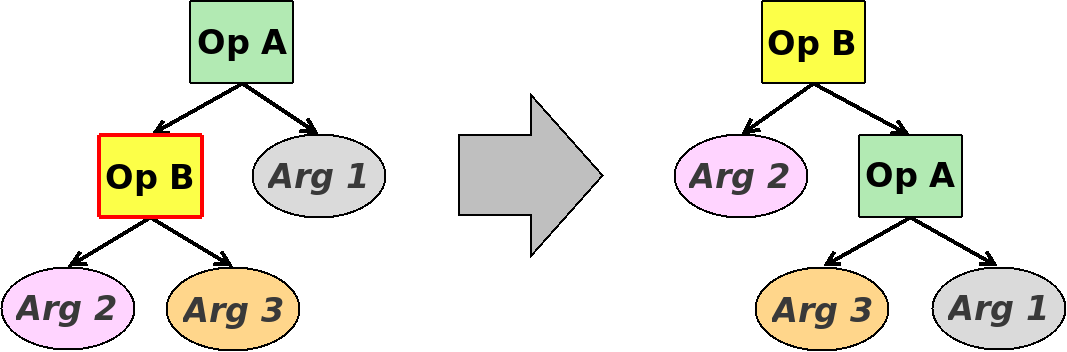
\includegraphics[width=250pt, height=82pt]{./rotacion1.png}
\caption{\label{rotacion1} Caso de rotación cuando la operación de la izquierda tiene menor precedencia.}
\end{figure}

\begin{figure}\centering
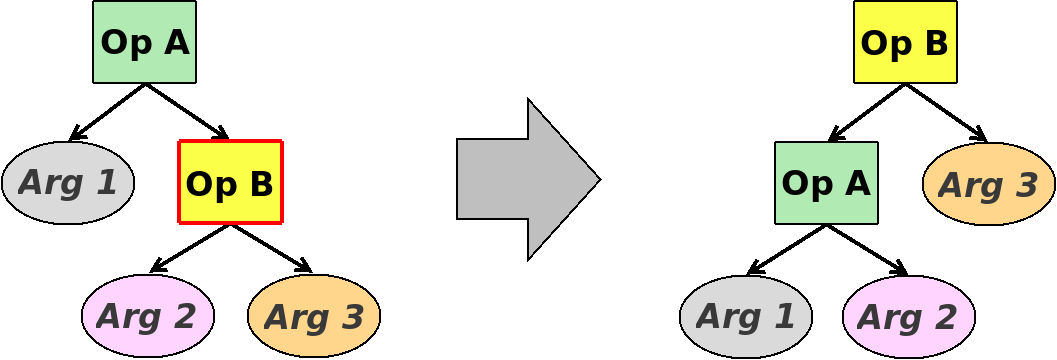
\includegraphics[width=250pt, height=85pt]{./rotacion2.png}
\caption{\label{rotacion2} Caso de rotación cuando la operación de la derecha tiene menor precedencia.}
\end{figure}

\begin{figure}\centering
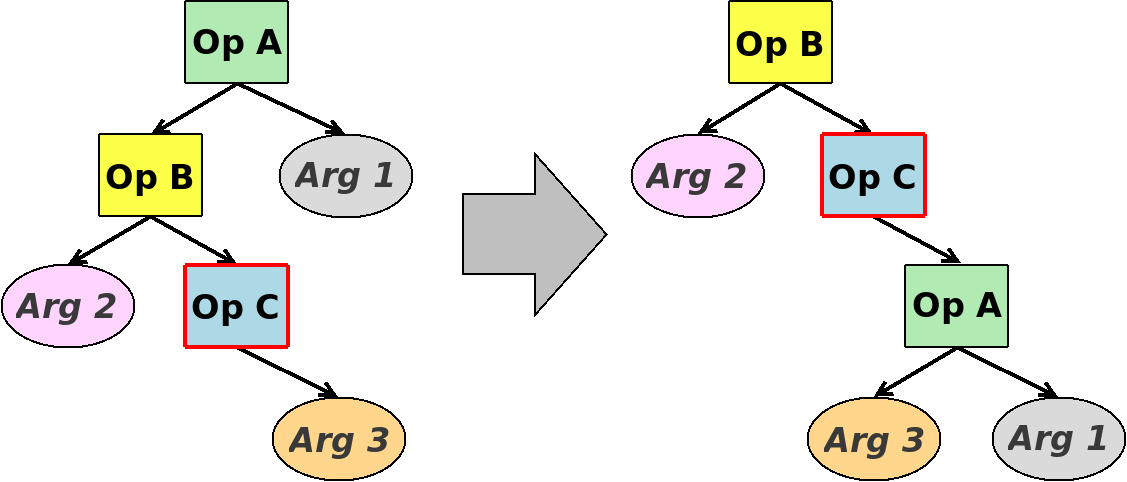
\includegraphics[width=250pt, height=107pt]{./rotacion3.png}
\caption{\label{rotacion3} Caso de rotación cuando se detectó un conflicto sin resolver.}
\end{figure}

Existen dos grandes casos a considerar:
\begin{itemize}
\item Si se inserta una operación infija, como hijo de otra operación, pero con menor precedencia que su padre, entonces se modificará el árbol, dejando como nueva raíz la operación infija recién insertada. 

Existen dos variantes, las cuales son presentadas en los diagramas \ref{rotacion1} y \ref{rotacion2}.

\item En cambio, cuando se inserta cualquier operación como hija de una operación prefija (raíz) y la insertada tiene mejor precedencia que la raíz, no se resuelve instantáneamente el error, dado que se alteraría el orden sintáctico de la expresión. Para ello se prende una bandera, a la cual se le asigna el valor de precedencia que tiene la operación recién insertada. Entonces cuando en el siguiente paso se agregue una nueva raíz, si tiene mayor precedencia que su ``nieto'' en el árbol, se realiza la siguiente rotación mostrada en el diagrama \ref{rotacion3}.
\end{itemize}

\subsection{Asociatividad de operadores dentro de expresiones}

El chequeo de la asociatividad y las eventuales modificaciones en el árbol de expresión, a diferencia del tratamiento que se le da a los problemas de precedencia, no se realiza a medida que se obtiene el árbol, sino que se lo aplica solamente una vez, cuando ya se terminó de parsear la expresión.

Esto se implementó así, ya que en ese punto, todos los elementos del árbol se encuentran posicionados respetando todas las precedencias, quedando potencialmente inconsistente la asociación de dos o más operadores infijos iguales, dentro del mismo nivel sintáctico, y con asociatividad a \textbf{derecha}, ya que por defecto todos los operadores son asociados a izquierda, debido al parser descendente recursivo que aplica \spirit.

Además, cuando se detectan dos operadores no asociativos se genera un error por mal uso de ese operador dentro de la expresión. Tal como se analizó en la sección XXX.

\subsection{Alcanzabilidad de símbolos y reglas}

En la especificación pueden existir de símbolos y reglas declaradas que no pueden ser alcanzados desde el símbolo inicial de la gramática. Los mismos no son útiles en la gramática ya que nunca producirán cadenas del lenguaje. Los mismos no son considerados errores pero son informados mediante alertas (\texttt{warnings}).

Este chequeo se implementó con una versión del algoritmo de Warshall\footnote{En honor a Stephen Warshall (1935 - 2006)}, que calcula la ``Clausura Transitiva'' de un grafo.

Para aplicarlo, primero se construye una matriz de valores lógicos reflejando todas las reglas declaradas. Luego de computar la clausura, se recorre la fila del símbolo inicial, que pertenece a la \textbf{única} regla inicial de la gramática por ser \textbf{extendida}. Todo símbolo que se encuentra con valor falso es inalcanzable.

\subsection{Consistencia de bloque de atributos y bloque de reglas}

Este chequeo consiste en verificar que no existan símbolos declarados en el bloque de atributos, que no hallan sido involucrados en ninguna regla. Esto puede suceder se crearon los símbolos de la expresión de conjuntos que define la pertenencia de un atributo.

La heurística utilizada, consiste en recorrer el \texttt{map} de símbolos no terminales y verificando que existe al menos una regla que lo tenga como parte izquierda.

\subsection{Gramática bien definida}

Este control es uno de los más importantes, ya que si la gramática por más que haya sido parseada correctamente, si no cumple con las condiciones de una MAG, nuestra herramienta la descarta y no le generará su correspondiente evaluador.

Como ya me sencionó en el capítulo XXX, varias son las condiciones que se deben chequear.

La heurística aplicada fue recorrer el \texttt{map} de reglas, donde para cada una verificábamos que estuviesen definidas dentro de su \texttt{map} de ecuaciones, una para cada uno de sus atributos sintetizados. Y a su vez, una ecuación para cada atributo heredado de sus símbolos de la parte derecha.

Además, también se controlara que no existieran ecuaciones incorrectas, es decir:
\begin{itemize}
\item Ecuaciones para atributos heredados del símbolo de la izquierda.
\item Ecuaciones para atributos sintetizados de símbolos de la parte derecha.
\end{itemize}

Cada vez que se detectaba un error, se lo informa mediante alguno de los siguientes mensajes según corresponda.

\texttt{\begin{itemize}
\item ``ERROR: ``E[1].syn1'' type synthetized, haven't an equation that defines it.''
\item ``ERROR: ``S[0].inh1'' type inherited, is defined outside his scope.''
\item ``ERROR: ``E[1].inh2'' type inherited, haven't an equation that defines it.''
\item ``ERROR: ``S[0].syn2'' type synthetized, is defined outside his scope.''
\end{itemize}}


\section{Obtención de planes de evaluación}

Como ya se explicó en el diseño, el propósito final de \maggen\ es obtener todos los planes posibles de la gramática de entrada.

Los planes están representamos como una secuencia de identificadores de ecuaciones. Utilizando la clase \texttt{vector} de la STL y manteniendo la unicidad en la enumeración de las ecuaciones.

Como en general, se iban a generar en muchos casos los mismos planes, se desidió mantener un \texttt{vector} con todos los planes diferentes, así solo generaríamos la mínima cantidad de planes únicos.

Como en el algoritmo que se presenta en el artículo de Wuu Yang(ver bibliografía XXX), a cada plan se lo asocia con un \texttt{key}, primero implementamos esa clave como una estructura con los siguientes datos:
\begin{itemize}
\item La regla a la cual pertenece el plan
\item Una secuencia para computar sus atributos
\end{itemize}

Esa secuencia se representó de igual manera que un plan, ya que computar un atributo es equivalente a saber el identificador de la ecuación que lo tiene como \texttt{l-value}.

El conjunto de estas secuencias, son los planes proyectados, es decir, las exigencias que se le imponen a una regla desde un contexto superior que la invoca a que se compute. Para el símbolo inicial, esta secuancia es obtenida como el órden topológico de su grafo DCG, ya que este contiene todas las dependencias entre los atributos de la regla, el cual si o si, será un órden de computación consistente para sus ecuaciones.

Al igual que con los planes de evaluación, los planes proyectados también sufrían de muchas repeticiones, por lo cual se usaron índices indirectos a un repositorio de los mismos almacenados en un \texttt{vector}.

Cada plan proyectado estaba bajo una clave particular, la cual según el algoritmo debía contener:
\begin{itemize}
\item La regla a la cual pertenece el plan proyectado
\item Una secuencia para computar sus atributos
\item El símbolo con el cual se proyento el plan de evaluación
\end{itemize}

Los dos primeros valores, corresponden a un \texttt{key} de un plan de evaluación, asi que se usó directamente esa estructura.

\subsection{Construcción de grafos}

Para la representación de los grafos uitlizamos la \boost\ \textit{\textbf{Graph Library}} (\textbf{BGL}). Ya que la misma presentaba muchas funcionalidades y ya se encontraba como una dependencia externa de la herramienta.

Como en la mayoria de los componentes de esta biblioteca, los mismos eran plantillas que necesitaban ser instanciados.

Las dependencias dentro de las reglas se dan entre las instancias de atributos de las ecuaciones y además los literales.

En la \textbf{BGL} los valores que se quieren asociar a los nodos, se vinculan mediante \textit{propiedades} inherentes a cada uno.

\begin{lstlisting}[language=C++, basicstyle=\scriptsize, numbers=left, numbersep=5pt, numberstyle=\tiny]
struct vertex_data_t
{
    typedef vertex_property_tag kind;
};
typedef property <vertex_data_t, const genevalmag::Expr_leaf*> property_vertex_dp;
typedef adjacency_list <hash_setS, vecS, directedS, property_vertex_dp> Graph;
typedef Graph::vertex_descriptor Vertex;
\end{lstlisting}

Se mantienen dentro de la herramienta un \texttt{map} para cada uno de los tipos de grafos necesarios y además para los subgrafos ADP cíclicos que eventualmente se detecten y para optimizar la construcción de los otros, los grafos que contienen todas las instancias de cada regla sin aristas entre si.

\begin{lstlisting}[language=C++, basicstyle=\scriptsize, numbers=left, numbersep=5pt, numberstyle=\tiny]
map <string, Graph>                 attr_vertex_graphs;
map <unsigned short, Graph>         p_Dp_graphs;
map <string, Graph>                 p_Down_graphs;
map <unsigned short, Graph>         p_Dcg_graphs;
map <vector<unsigned short>, Graph> p_Adp_graphs;
map <vector<unsigned short>, Graph> p_Adp_subgraphs_cyclics;
\end{lstlisting}

El chequeo de ciclicidad sobre los grafos ADP, se implementó utilizando el algoritmo de búsqueda en profundidad (Depth-first search) de \boost\ combinado con la creación de un ``visitador'' especilizado que a medida recorre el grafo, va guardado los nodos y aristas visitadas mientras no se halla detectado un ciclo. Ese subgrafo es lo que se guarda y se muestra al usuario.

La detección de ciclos se realiza cuando el algoritmo invoca a la función \texttt{back\_edge}, en donde nosotros prendemos una bandera.

Tanto el grafo como la variable lógica, usada como bandera, son pasadas en el constructor y utilizadas internamente mediante referencias.

\begin{lstlisting}[language=C++, basicstyle=\scriptsize, numbers=left, numbersep=5pt, numberstyle=\tiny]
struct cycle_detector: public dfs_visitor<>
{
  public:
    cycle_detector(bool& has_cycle, Graph &graph):
      _has_cycle(has_cycle),
      _graph_cycle(graph)
    {}

    template <class Edge, class G>
    void examine_edge(Edge u, const G &g)
    {
      if(!_has_cycle)
      {
        ...
      }
    }

    template <class Edge, class G>
    void back_edge(Edge u, const G& g)
    {
      _has_cycle = true;
    }

  protected:
    bool   &_has_cycle;
    Graph  &_graph_cycle;
};
\end{lstlisting}

Para cada regla, se tienen que considerar todos los posibles contextos inferios posibles de acuerdo a las reglas que tengan los símbolos no terminales de su parte derecha. Se implementó un método que recursivamente genera un contexto diferente y guarda la regla cuando ya no quedan más variantes.

Al igual que con los planes, los contextos de las reglas se repiten mucho, así que se utilizaron índices indirectos sobre un \texttt{vector} que almacena unicamente los contextos diferentes.

\begin{lstlisting}[language=C++, basicstyle=\scriptsize, numbers=left, numbersep=5pt, numberstyle=\tiny]
vector < Order_rule >    contexts_uniques;
vector < Order_eval_eq > plans_uniques;
vector < Order_eval_eq > plans_project_uniques;
\end{lstlisting}

Antes de insertar un elemento en cualquiera de estos repositorios se verifica que no exista. En caso de que ya se encuentre, se devuelve el índice correspondiente dentro del vector, sino se insertará al final y se devolverá el índice del último elemento.

Una vez que se generaron todos los tipos de grafos, los mismos son guardados en distintos directorios en formato \textbf{dot}\cite{dot}. Para ello utilizamos la función \texttt{write\_graphviz} perteneciente a al módulo Graphviz de \boost.


\section{Algoritmo de Computar Planes de Wuu Yang}

\begin{lstlisting}[basicstyle=\footnotesize, escapeinside=<>, language=inform]
Algorithm: ComputePlan

WL := <$\emptyset$>
<$\Delta$> := a function that is undefined in every place
<$\mu$> := an arbitrarily chosen evaluation order of the start symbol's attributes

for each production q whose left-hand-side nonterminal is the start symbol S do
  WL := WL <$\cup$> { (q , <$\mu$>) }
end for

repeat
  repeat
    (q, <$\omega$>) := an element of WL
    WL := WL - { (q, <$\omega$>) }
  until <$\Delta$>(q, <$\omega$>) = undefined
  
  <$\Delta$> := [<$\Delta$> | <$\Delta$>(q, <$\omega$>) = defined ]
  
  Let production q be denoted by X<$_{0}$> <$\rightarrow$> <$\alpha_{0}$>X<$_{1}$><$\alpha_{1}$>X<$_{2}$><$\alpha_{2}$> <$\ldots$> X<$_{k}$><$\alpha_{k}$>.
  
  for each ADP (q | p<$_{1}$>, p<$_{2}$>, <$\ldots$> , p<$_{k}$>) <$\in$> SADP (q) do
    <$\psi$> := ComputeOrder (ADP (q | p<$_{1}$>, p<$_{2}$>, <$\ldots$> , p<$_{k}$>), <$\omega$>)
    <$\gamma$>[q , <$\omega$>, p<$_{1}$>, p<$_{2}$>, <$\ldots$> , p<$_{k}$>] := <$\psi$>
    for each nonterminal X<$_{i}$> appearing on the right-hand-side of production q do
      <$\psi_{i}$> := project (<$\psi$>, {X<$_{i}$>'s attribute occurrences})
      <$\theta$>[q , <$\omega$>, i , p<$_{1}$>, p<$_{2}$>, <$\ldots$> , p<$_{k}$>] := <$\psi_{i}$>
      if <$\Delta$>(<$p_{i}$>, <$\psi_{i}$>) = undefined then
        WL := WL <$\cup$> { (<$p_{i}$>, <$\psi_{i}$>) }
      end if
    end for
  end for
until WL = <$\emptyset$>
\end{lstlisting}

\normalsize
     % Implementación.
\chapter{Usando \maggen}
\label{chap:usos}
\minitoc

Para usar \maggen\ se debe invocar la herramienta mediante la línea de comando, es decir, por lo se es necesario contar con una terminal\footnote{En sistemas \textit{Windows} compatible: \textbtt{Win+R} y luego \textbtt{cmd} y en sistemas \textit{Unix}: \textbtt{Alt+F2} y luego \textbtt{xterm}.} para su ejecución. Por cuestiones de simplicidad y flexibilidad de la herramienta, no se consideró el desarrollo de un \textit{front-end} para \maggen. Además, se debe tener en cuenta, que el usuario debería presentar mayor interés en el resultado producido por \maggen\ y no de una innecesaria interfaz gráfica, que entorpecería su comportamiento combinatorio con otros comandos.
  
\maggen\ puede ser invocado utilizando una serie de parámetros que inciden directamente sobre el resultados producido por la herramienta. En el desarrollo de este capítulo se tratarán estos temas en detalles y además se analizará el uso del evaluador generado por \maggen.

\section{Compilación e Instalación de \maggen}
\maggen\ puede ser descargado desde el repositorio svn (\cite{svn-book}) utilizando el siguiente comando:
\begin{verbatim}
 svn checkout http://genevalmag.googlecode.com/svn/trunk/ maggen
\end{verbatim}

Una vez descargado la última versión de \maggen, se dispondrá de un directorio llamado ``\textbtt{maggen/}'', dentro del cual se alojan todos los archivos de la herramienta.

Para compilar \maggen, primero el usuario deberá posicionarse dentro del directorio ``\textbtt{maggen/}'', mediante las funciones de la terminal, y luego deberá ejecutar los siguientes comandos:
{\small\begin{verbatim}
 1.- user@pc:~/maggen$ cmake .
 2.- user@pc:~/maggen$ make clean
 3.- user@pc:~/maggen$ make
\end{verbatim}}
La compilación de \maggen\ se realiza mediante el comando ``\textbtt{cmake}'', detalles sobre esta herramienta fueron presentados en la sección \ref{sec:metoherram}. 
En la figura \ref{fig:cmake_maggen} y \ref{fig:make_maggen} se puede ver la ejecución de los comandos 1 y 3.
\begin{figure}[!ht]\centering
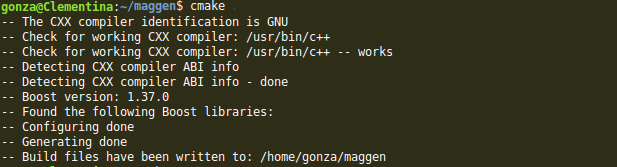
\includegraphics[width=300pt,height=105pt]{cmake_maggen.png}
\caption{\label{fig:cmake_maggen} Ejecución de ``\textbtt{cmake}'' en la terminal de comandos.}
\end{figure}

\begin{figure}[!ht]\centering
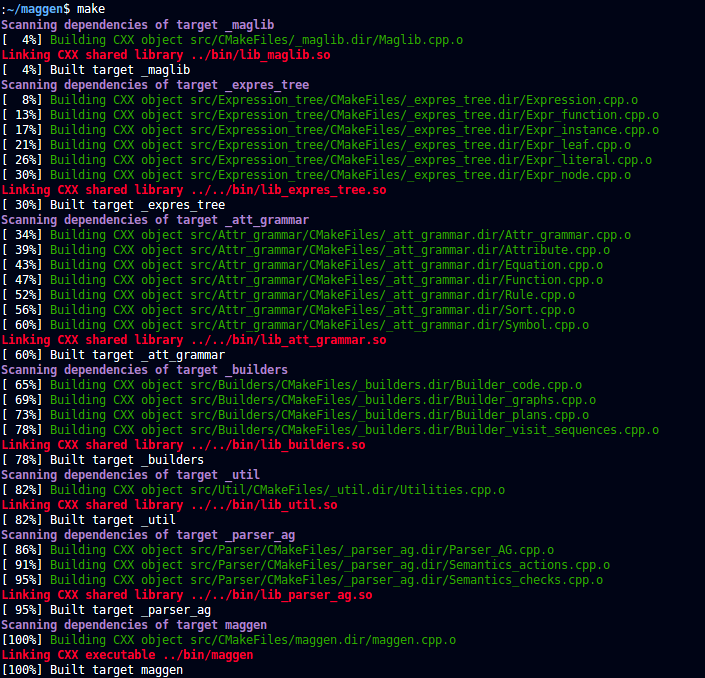
\includegraphics[width=300pt,height=301pt]{make_maggen.png}
\caption{\label{fig:make_maggen} Ejecución de ``\textbtt{make}'' en la terminal de comandos.}
\end{figure}
 
\subsection{Directorio \textbtt{maggen}}
Luego de la compilación e instalación, el directorio raíz de \maggen\ se compone de lo siguiente:
\begin{itemize}
\item \textbtt{/bin} Directorio que contiene módulos estáticos necesarios para la ge\-ne\-ración de código y uso del evaluador obtenido.
{\footnotesize \begin{verbatim}
 user@pc:~/maggen$ ls -R bin/
 bin:
 lib

 bin/lib:
 Node.hpp  Plan.hpp
\end{verbatim} }
 
\item \textbtt{/src} Directorio raíz en el que se encuentran todos los archivos fuentes.
{\footnotesize \begin{verbatim}
 user@pc:~/maggen$ ls -R src/ 
 src/:
 Attr_grammar  Builders  Expression_tree  maggen.cpp  Maglib.cpp  
 Parser  Util CMakeLists.txt

 src/Attr_grammar:
 Attr_grammar.cpp  Attribute.cpp  Equation.cpp  Function.cpp  
 Rule.cpp  Sort.cpp  Symbol.cpp CMakeLists.txt

 src/Builders:
 Builder_code.cpp  Builder_graphs.cpp  Builder_plans.cpp  
 Builder_visit_sequences.cpp CMakeLists.txt

 src/Expression_tree:
 Expression.cpp  Expr_function.cpp  Expr_instance.cpp  
 Expr_leaf.cpp  Expr_literal.cpp  Expr_node.cpp CMakeLists.txt

 src/Parser:
 Parser_AG.cpp  Semantics_actions.cpp  Semantics_checks.cpp
 CMakeLists.txt

 src/Util:
 Utilities.cpp CMakeLists.txt
\end{verbatim} }

\item \textbtt{/include} Directorio raíz en el que se encuentran todos los archivos de cabecera.

{\footnotesize \begin{verbatim}
 user@pc:~/maggen$ ls -R include/
 include/:
 Attr_grammar  Builders  Expression_tree  Maglib.h  
 Parser  Util

 include/Attr_grammar:
 Attr_grammar.h  Attribute.h  Equation.h  Function.h  
 Rule.h  Sort.h  Symbol.h

 include/Builders:
 Builder_code.h  Builder_graphs.h  Builder_plans.h  
 Builder_visit_sequences.h

 include/Expression_tree:
 Expression.h  Expr_function.h  Expr_instance.h  
 Expr_leaf.h  Expr_literal.h  Expr_node.h

 include/Parser:
 Parser_AG.h  Semantics_actions.h  Semantics_checks.h

 include/Util:
 Utilities.h
\end{verbatim}}

\item \textbtt{/scripts} Directorio que contiene scripts útiles para el usuario, por e\-jem\-plo: \textbtt{dot2png.sh} para convertir a imagen \textit{png} los archivos de grafos y planes generados por \maggen.
{\footnotesize \begin{verbatim}
 user@pc:~/maggen$ ls -R scripts/
 scripts/:
 dot2png.sh
\end{verbatim} }
 
\item \textbtt{/examples} En este directorio se encuentran tres ejemplos de gramáticas para probar la herramienta. Uno de ellos es el tratado en el desarrollo de este informe, presentado en el apéndice \ref{append:agwuuyang}. 
{\footnotesize \begin{verbatim}
 user@pc:~/maggen$ ls -R examples/
 examples/:
 ag_aritmetic  ag_count  ag_wuu_yang

 examples/ag_aritmetic:
 ag_aritmetic.cpp  ag_aritmetic.input

 examples/ag_count:
 ag_count.cpp  ag_count.input

 examples/ag_wuu_yang:
 ag_wuu_yang.cpp  ag_wuu_yang.input
\end{verbatim} }

\item \textbtt{/doc} Directorio que contiene la documentación de la herramienta (doxygen).
% \item \textbf{/Release} Directorio con los archivos compilados.

\item Archivo \textbtt{CMakeLists.txt} usado por \textbtt{cmake} para generar los archivos \textbtt{Makefile} que permiten automatizar el proceso de compilación, empaquetado el proyecto.
\end{itemize}

En este momento, ya esta todo preparado para empezar a usar \maggen, en las siguientes secciones se analiza como usar la herramienta.

\section{Uso de \maggen: Parámetros y opciones}
\label{sec:uso-maggen}
La totalidad de parámetros y opciones de \maggen\ son opcionales. La sintaxis de invocación de la herramienta esta dada por:\\
\begin{center}\textbtt{maggen [OPTIONS]}\end{center}

Las opciones son las siguientes:

\begin{description}
\item [\textbtt{-f  file}] Definir el archivo de entrada de \maggen\ como \textbtt{file}. Si se omite esta opción \maggen\ espera la entrada por la entrada estándar (\textbtt{cin}) hasta leer el carácter \textbtt{EOF} (End Of File)\footnote{En sistemas \textit{Unix} el carácter \textbtt{EOF} puede ser producido con \textbtt{Ctrl+D} dentro de una consola de comandos.}.

\item [\textbtt{-i  header}] Incluir \textbtt{header} en la generación de código. Genera un \textbtt{\#include ``header''} del archivo que referencia esa ruta. Dicha línea, \maggen\ la agrega al archivo generado.

\item [\textbtt{-fo folder}] Define \textbtt{folder} como el directorio de salida para \maggen. Si se omite esta opción, \maggen\ usa el folder por defecto ``\textit{./out\_maggen/}''.

\item [\textbtt{-o  name}] Define a \textbtt{name} como el nombre de la clase y del archivo generado por \maggen. Si se omite esta opción, \maggen\ usa por defecto el nombre ``\textbf{mag\_eval}''.

\item [\textbtt{-h}] Muestra mensaje de ayuda.
\end{description}

A continuación se observan algunos ejemplos de invocación de \maggen.
\begin{itemize}
\item Si se invoca:
\begin{center}{\textbtt{./maggen -h}}\end{center} se obtiene el siguiente mensaje de ayuda:

\begin{figure}[!ht]\centering
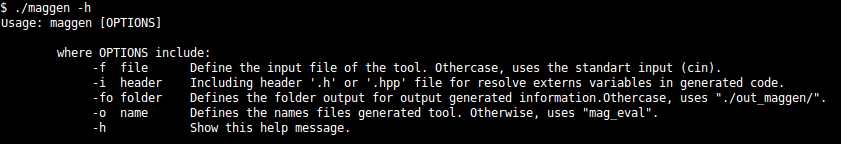
\includegraphics[width=350pt,height=60pt]{help.png}
\caption{\label{fig:outhelp} Información de ayuda de \maggen.}
\end{figure}

\item Si se invoca:  \begin{center}
{\scriptsize\textbtt{./maggen -fo ./out\_wuu\_yang -o evalmag -f ./examples/ag\_wuu\_yang/ag\_wuu\_yang.input}}                                                                                                                                   \end{center} Si se especifica como archivo de entrada a \textbtt{ag\_wuu\_yang.input}, como directorio de salida \textbtt{./Out\_wuu\_yang} y el nombre de la clase (y archivo) generada con el nombre \textbtt{evalmag}. La figura \ref{fig:outnormal} muestra la salida de esta invocación.

\begin{figure}[!ht]\centering
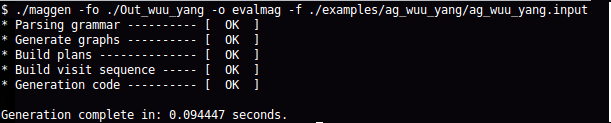
\includegraphics[width=350pt,height=69pt]{normal.png}
\caption{\label{fig:outnormal} Usando \maggen\ con opciones.}
\end{figure}

\item Si se invoca a \maggen\ sin la opción \textbtt{-f} (independientemente que se usen, o no, las demás opciones) se espera la entrada por entrada estándar. Esto permite poder utilizar a \maggen\ en conjunto con otros comandos de forma encadenada. Por ejemplo:

\begin{center}\textbtt{cat file | maggen -fo ./out/}.\end{center}

Esto muestra a \maggen\ en conjunto con \textbtt{cat} usando una tubería (\textbtt{pipe}, en ambientes \textit{Unix} mediante el operador ``\textbtt{|}'').

\end{itemize}

La salida de \maggen\ esta ordenada a través de directorio bien definidos que marcan el proceso de funcionamiento de la herramienta en cada etapa. A continuación se analizarán la salida de \maggen\ para siguiente invocación:

\begin{center}{\scriptsize\textbtt{./maggen -fo ./Out\_wuu\_yang -o maggen -f ./examples/ag\_wuu\_yang/ag\_wuu\_yang.input}}\end{center}

La totalidad de la información generada por la herramienta es mostrada en la figura \ref{fig:outmaggen}.

\begin{figure}[!ht]\centering
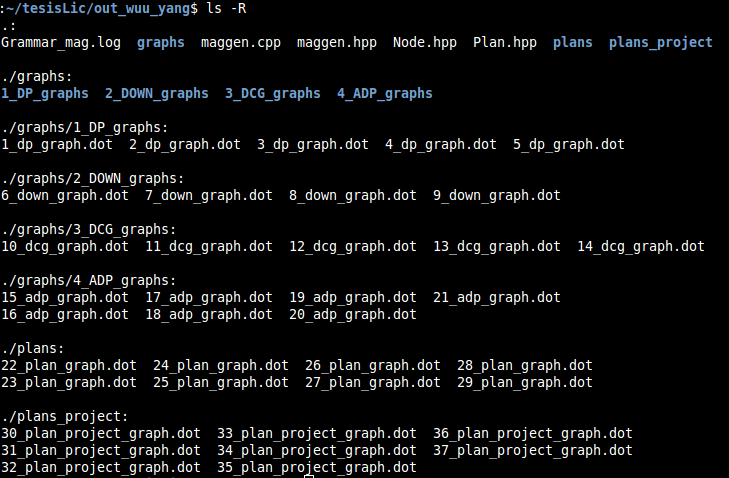
\includegraphics[width=350pt,height=229pt]{out_all.png}
\caption{\label{fig:outmaggen} Salida de \maggen: Directorios y archivos.}
\end{figure}

Dicha información es almacenada en la ruta \textbtt{./Out\_wuu\_yang}, dentro de la cual se encuentran:

\begin{description}
\item [Archivos \textbtt{maggen.cpp} y \textbtt{maggen.cpp}] Código C++ del evaluador estático. Es la \emph{salida principal} de \maggen.

\item [Archivos \textbtt{Plan.hpp} y \textbtt{Node.hpp}] Código C++ con definiciones y declaraciones necesarias para la ejecución de ``\maggen''.

\item [Archivo ``\textbtt{Grammar\_mag.log}''] Este contiene la gramática parseada. Se debe tener en cuenta el análisis de este archivo, esto permite encontrar posibles errores en la interpretación del archivo de entrada a \maggen. Tal como se muestra la gramática en este archivo, es la que la herramienta a utilizado para la generación del evaluador.

\item [Directorio ``\textbtt{graphs}''] Contiene los 4 tipos de grafos construidos por \maggen\ en el proceso visto en la sección \ref{subsec:graph}. Los mismos están ordenados por 4 directorios diferentes denominados: \textbtt{1\_DP\_graphs}, \textbtt{2\_DOWN\_graphs}, \textbtt{3\_DCG\_graphs}, \textbtt{4\_ADP\_graphs}. Cada unos de ellos contiene archivos \textbtt{.dot} para cada grafo creado. Este directorio, además, es utilizado para el caso en que se detecten planes cíclicos, para almacenar los grafos que producen dependencias cíclicas en un solo directorio y se omiten los demás grafos.

\item [Directorio ``\textbtt{plans}''] Contiene archivos \textbtt{.dot} con los planes generados por \maggen.

\item [Directorio ``\textbtt{plans\_project}''] Contiene archivos \textbtt{.dot} con los planes proyectados generados por \maggen.
\end{description}

\section{Uso del evaluador generado}

Para el uso del evaluador generado por \maggen\ se necesitan los 4 archivos generados en el directorio de salida. Tomando una de las salidas de la sección anterior, ellos son:
\begin{items}
\item \textbtt{maggen.hpp}.
\item \textbtt{maggen.cpp}.
\item \textbtt{Plan.hpp}.
\item \textbtt{Node.hpp}.
\end{items}

El evaluador generado por \maggen\ puede ser usado como un módulo C++ dentro de otro proyecto. En esta sección se continuará con un ejemplo de Wuu Yang, el cual ya se ha tratado en los capítulos anteriores (Ver especificación de entrada a \maggen\ en el apéndice \ref{append:agwuuyang}).

Como bien se ha visto en secciones anteriores, la entrada del evaluador generado por \maggen\ debe ser un AST. El siguiente archivo C++ construye un AST para la gramática del ejemplo de Wuu Yang, y luego lo pasa al e\-va\-lua\-dor para que lo decore.

\lstinputlisting[numbers=left]{input_file_code/ag_wuu_yang.cpp}

El siguiente diagrama representa el AST a evaluar:

\begin{center}
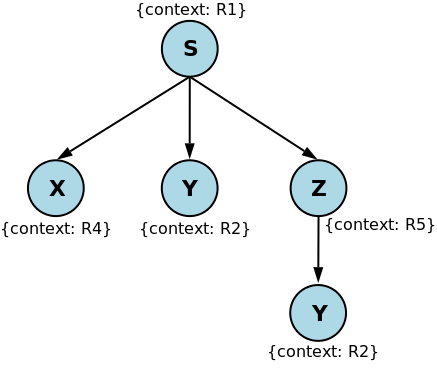
\includegraphics[width=200pt,height=154pt]{ast.png}
\end{center}

Los atributos de cada símbolo del AST se encuentran con valores indefinidos, pero luego de la compilación y ejecución, en la cual se invoca al evaluador generado por \maggen, como se ve en la siguiente imagen ahora tienen definidos sus respectivos valores calculados.

\begin{center}
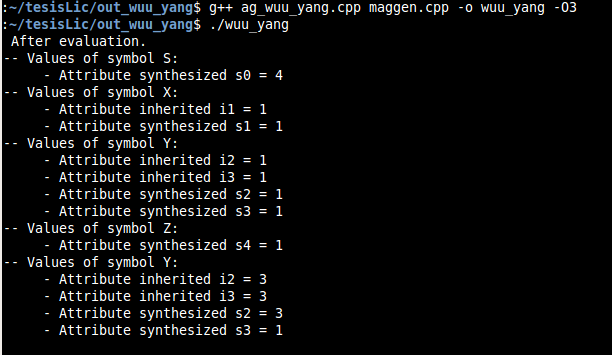
\includegraphics[width=350pt,height=203pt]{ast-computed.png}
\end{center} 

En la siguiente tabla se analizan los valores de los atributos de cada símbolo:

\begin{center}\begin{tabular}{|| c | c | l ||}
\hline \hline

\rowcolor{gris} \textbf{Símbolo}&\textbf{Atributo}&\textbf{Evaluación}\\ \hline

\multirow{2}{*}{\textbf{S}} & \multirow{2}{*}{s0} & \textbtt{(eq 1) S.s0 = X.s1 + Y.s2 + Y.s3 + Z.s4} \\ 
                           &                     & \textbf{S.s0 = 4} \\ \hline

\multirow{4}{*}{\textbf{X}} & \multirow{2}{*}{i1} & \textbtt{(eq 2) X.i1 = Y.s3} \\ 
                            &                     & \textbf{X.i1 = 1.} \\ \cline{2-3}
                            & \multirow{2}{*}{s1} & \textbtt{(eq 9) X.s1 = X.i1} \\ 
                            &                     & \textbf{X.s1 = 1.} \\ \hline

\multirow{7}{*}{\textbf{Y}} &                 s3  & \textbtt{(eq 6)} \textbf{Y.s3 = 1} \\ \cline{2-3}
                            & \multirow{2}{*}{s2} &    \textbtt{(eq 5) Y.s2 = Y.i2} \\
                            &                     & \textbf{Y.s2 = 1} \\ \cline{2-3}
                            & \multirow{2}{*}{i2} & \textbtt{(eq 3) Y.i2 = X.s1} \\
                            &                     & \textbf{Y.i2 = 1} \\ \cline{2-3}
                            & \multirow{2}{*}{i3} & \textbtt{(eq 4) Y.i3 = Y.s2} \\
                            &                     & \textbf{Y.i3 = 1} \\ \hline

\multirow{2}{*}{\textbf{Z}} & \multirow{2}{*}{S4} & \textbtt{(eq 10) Z.s4 = Y.s3} \\
                            &                     & \textbf{Z.s4 = 1} \\ \hline

\multirow{7}{*}{\textbf{Y}} &                  s3 & \textbtt{(eq 6)} \textbf{Y.s3 = 1} \\ \cline{2-3}
                            & \multirow{2}{*}{s2} &    \textbtt{(eq 5) Y.s2 = Y.i2} \\
                            &                     & \textbf{Y.s2 = 3} \\ \cline{2-3}
                            & \multirow{2}{*}{i2} & \textbtt{(eq 3) Y.i2 = X.s1} \\
                            &                     & \textbf{Y.i2 = 3} \\ \cline{2-3}
                            & \multirow{2}{*}{i3} & \textbtt{(eq 4) Y.i3 = Y.s2} \\
                            &                     & \textbf{Y.i3 = 3} \\
\hline \hline
\end{tabular}\end{center}

Tal como se analizó en el ejemplo anterior, el evaluador generado por \maggen\ podría ser utilizado con todos lo AST posibles. Esto es, debido a que el evaluador contiene las secuencias de visita previamente computadas para hacer la tarea de evaluación con una notoria ganancia de tiempo. Entonces se podría invocar al evaluador, además, con los demás AST que se desprenden con la gramática del ejemplo de Wuu Yang. En la figura \ref{fig:allast} se puede ver la totalidad de ASTs.

\begin{figure}[!ht]\centering
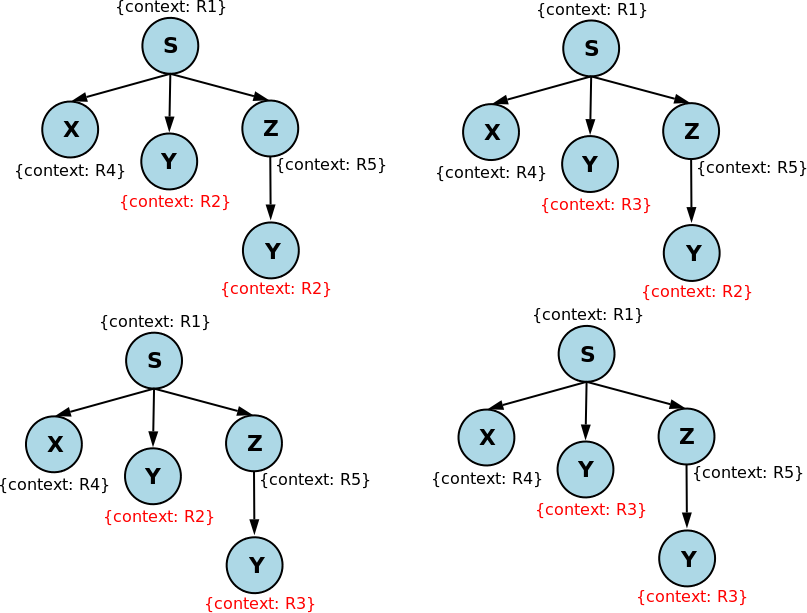
\includegraphics[width=350pt,height=266pt]{ast-all.png}
\caption{\label{fig:allast} AST para ejemplo de Wuu Yang.}
\end{figure}

Notar que el ejemplo Wuu Yang analizado es considerablemente sencillo, pero se puede encontrar gramáticas muy simples en la cual los posibles ASTs sea una cantidad considerable, es en este punto donde el evaluador generado por \maggen\ adquiere mayor potencial y utilidad.

\section{Mensajes y avisos}

En los cuadros \ref{table:mensajes-err} y \ref{table:mensajes-av} se analizarán la descripción de los posibles errores y avisos que se deben tener en cuenta cuando se usa \maggen.

% \begin{table}
\begin{small}
\begin{longtable}{| p{4.5cm} || p{4.5cm} | p{4.5cm} |}
\hline
\hline

\rowcolor{gris} \textbf{Mensaje} & \textbf{Descripción} & \textbf{Ayuda} \\ \hline \hline

ERROR: operator non-associtive using wrong use: \textit{OP} & El operador \textit{OP} es non\_assoc y se pretende una asociación del mismo, en alguna expresión. & Modifique la definición del operador o chequee la expresión.\\ \hline

ERROR: Symbol Non-Teminal \textit{SYMB} uses in the right part without rule & El símbolo \textit{SYMB}, usado en la gramática, no tiene regla que lo defina. & Chequee los símbolos usados o defina una regla para el símbolo \textit{SYMB}. \\ \hline

ERROR: \textit{SYMB} [\textit{NUM}]. \textit{ATTR} type synthetized, haven't an equation that defines it. & Gramática mal definida, atributo sintetizado \textit{ATTR} sin ecuación que lo defina. Para más información chequee la sección \ref{subsec:check} & Defina ecuación para la instancia o chequee la definición de la gramática. \\ \hline

ERROR: \textit{SYMB} [\textit{NUM}].\textit{ATTR} type inherited, haven't an equation that defines it. & Gramática mal definida, atributo heredado \textit{ATTR} sin ecuación que lo defina. Para más información chequee la sección \ref{subsec:check} & Defina ecuación para la instancia o chequee la definición de la gramática. \\ \hline

ERROR: \textit{SYMB} [\textit{NUM}].\textit{ATTR} type synthetized, is defined outside his scope. & La instancia \textit{SYMB} [\textit{NUM}].\textit{ATTR} esta definida fuera de su regla de alcance. & Defina ecuación en el alcance de la regla o chequee la instancia usada. \\ \hline

ERROR: the file input non-exist & El archivo de entrada a \maggen\ no existe o es inaccesible. & Chequee la ruta del archivo de entrada. \\ \hline

ERROR: Parsing Failed, the following text will not be able to parse: \ldots & Error sintáctico en la definición de la gramática. Para más información chequee la sección \ref{sec:lenguajeMAG} & Revise la sintaxis del lenguaje de definición para \maggen\ y modifique su definición. \\ \hline

ERROR: non-terminal symbol \textit{SYMB} used does not belong to the rule: \textit{R} & Instancia utilizada fuera de su entorno. Símbolo de la instancia no pertenece al entorno de la regla. & Revise el uso de la instancia o modifique la regla \textit{R}.  \\ \hline

ERROR: Index \textit{NUM} of symbol  \textit{SYMB} incorrect. & Índice \textit{NUM} de instancia fuera de rango. No corresponde el índice con el orden sintáctico del símbolo en la regla. & Revise el índice \textit{NUM} o modifique la definición de la regla.  \\ \hline 

ERROR: \textit{ATTR} Attribute non-existent. Check the attributes used in the symbols. & El atributo no pertenece al símbolo. & Defina el atributo \textit{ATTR} o modifique el uso de esa instancia. \\ \hline

ERROR: Type not expected from l\_value." & Error de tipo. El tipo que sintetiza la expresión r\_value no corresponde con el tipo de l\_value & Revise la expresión en busca de mal uso de operadores, o modifique los tipos de los atributos u operadores. \\ \hline
 
ERROR: infix operator non-exist: \textit{OP-IN}. & El operador infijo \textit{OP-IN} utilizado en la expresión no esta definido o esta siendo usado con tipos erróneos. & Defina el operador o modifique la expresión. \\ \hline
 
ERROR: Function non-exist: \textit{F}. & La función \textit{F} utilizada en la expresión no esta definida o esta usada con tipos erróneos. & Defina la función o modifique la expresión. \\ \hline
 
ERROR: postfix operator non-exist: \textit{OP-POS}. & El operador posfijo \textit{OP-POS} utilizado en la expresión no esta definido o esta usado con tipos erróneos. & Defina el operador o modifique la expresión. \\ \hline 

ERROR: prefix operator non-exist: \textit{OP-PRE}. & El operador prefijo \textit{OP-PRE} utilizado en la expresión no esta definido o esta usado con tipos erróneos. & Defina el operador o modifique la expresión. \\ \hline 

ERROR: The grammar isn't extended grammar. & Error en la definición de la gramática, la misma no cumple con la propiedad de gramática extendida. Ver detalles en sección \ref{sec:def-CFG} & Chequee la definición de la gramática para que cumpla la propiedad.(sección grammar extended) \\ \hline

ERROR: the path \textit{PATH} is invalid or inaccessible. & El camino (PATH) es inexistente o inaccesible. & Verifique la ruta e invoque a \maggen\ nuevamente. \\ \hline

ERROR: One o more graph ADP has an cycle in its dependencies. Look the folder \textit{PATH-OUTPUT}. & El proceso de \maggen\ tuvo que ser abortado, debido a la existencia de planes con dependencias circulares. & Chequee la definición de las ecuaciones que se vinculan con los grafos mostrados en \textit{PATH-OUTPUT}. \\ \hline 

ERROR: Path non exist: \textit{PATH}. & Ruta errónea o inaccesible. & Modifique la ruta PATH o ingrese una nueva. \\ \hline 

ERROR: maggen wrong uses. & Mal uso de \maggen, uno de los argumentos es erróneo, en la invocación. & Modifique los argumentos. Para más detalles chequee sección \ref{sec:uso-maggen} \\ \hline

ERROR: Index out bounds: combined ADP graphs.& Error fatal en la generación de contextos para la construcción de ADP. & Chequee la entrada a \maggen.\\ 
\hline
\hline
\caption{\label{table:mensajes-err}Tabla con mensajes de error en \maggen.}
\end{longtable}
\end{small}
% \end{table}

% \begin{table}
\begin{small}
\begin{longtable}{| p{4.5cm} || p{4.5cm} | p{4.5cm} |}
\hline
\hline

\rowcolor{gris} \textbf{Mensaje} & \textbf{Descripción} & \textbf{Ayuda} \\ \hline \hline

WARNING: Symbol Non-Teminal  \textit{SYMB} unreachable. & El símbolo \textit{SYMB} es inalcanzable desde la regla inicial de la gramática. El mismo es ignorado en el proceso de cómputo. & Chequee la gramática de entrada a \maggen\ o elimine el símbolo en caso de uso innecesario. \\ \hline

WARNING: Sort duplicate was ignored: $-->$ \textit{S} & La declaración del sort \textit{S} esta duplicada. \maggen\ ignora dicha línea. & Elimine la declaración del sort \textit{S} o modifique la misma en caso de declaración de sort distinto. \\ \hline

WARNING: Declaration duplicate was ignored: $-->$ \textit{F} & La declaración de la función \textit{F} esta duplicada. \maggen\ ignora dicha línea. & Elimine la declaración de la función \textit{F} o modifique la misma en caso de declaración de función distinta. \\ \hline

WARNING: Ignores the eq \textit{E} duplicate definition for \textit{IN} in rule: $-->$ \textit{R} & La ecuación \textit{E} para la instancia \textit{IN} en la regla \textit{R} es ignorada por \maggen, debido a que la instancia \textit{IN} ya tiene ecuación que la defina. & Chequee las ecuaciones que definen la instancia \textit{IN} y elimine una o verifique posibles errores en la ecuación. \\
\hline
\hline
\caption{\label{table:mensajes-av}Tabla con mensajes de avisos en \maggen.}
\end{longtable}
\end{small}
% \end{table}

% \normalsize

En los cuadros anteriores se pudo analizar los errores y avisos en el uso de \maggen. Esta diferencia en los mensajes, se hace en el sentido de que, los avisos, no son considerados errores fatales en el proceso de la herramienta y por ende no es necesario abortar el funcionamiento. Los errores considerados avisos, \textbf{son ignorados} dentro del funcionamiento interno de \maggen.

Al igual como se analizó para \maggen, en la tabla \ref{table:mensajes-err-eval} se mostrarán los mensajes de error que pueden aparecer con en el uso del evaluador generado.

% \begin{table}
\begin{small}
\begin{longtable}{| p{4.5cm} || p{4.5cm} | p{4.5cm} |}
\hline
\hline

\rowcolor{gris} \textbf{Mensaje} & \textbf{Descripción} & \textbf{Ayuda} \\ \hline

ERROR: the AST input is wrong create. Context rule does not exist. & Los nodos del AST describen una combinación de reglas no posible en la gramática de entrada. & Revise el AST o modifique la gramática y genere nuevamente el evaluador con \maggen. \\ \hline

ERROR: the AST input is wrong create. Evaluation plan does not exist. & El orden de evaluación impuesto al nodo no corresponde. & Revise si la gramática esta bien especificada. \\ \hline

ERROR: Fatal action. & Se desea invocar a la computación de una ecuación errónea e inexistente. & Chequee el AST de entrada al evaluador. \\
\hline
\hline
\caption{\label{table:mensajes-err-eval}Mensajes de error del evaluador generado.}
\end{longtable}
\end{small}
% \end{table}

El error más importante y común cuando se usa el evaluador generado por \maggen\ esta dado por el AST de entrada. Es aconsejable que se chequee de manera exhaustiva la creación de estos AST para evitar complicaciones.
       % Usos de magGen.
\chapter{Conclusión y trabajos futuros}
\label{chap:conclusiones}

\minitoc

En el desarrollo del presente capítulo se presentarán comentarios finales del proyecto y además, posibles extensiones y trabajos a futuro.

\section{Conclusión}

En esta sección se expondrán las conclusiones obtenidas luego del desarrollo de este proyecto.\\

Durante todo el desarrollo de este trabajo se ha estudiado e introducido conocimientos sobre \textit{Gramáticas de Atributos}, desde el punto de vista de definiciones, como así también de problemáticas y estado actual de desarrollo de las mismas. Además, se ha trabajado con una familia de GA, relativamente nuevas, como lo son las Multi-planes (MAG), presentas por Wuu Yang (1998). Sobre estas es posible desarrollar evaluadores estáticos mediante técnicas que se apoyan en secuencias de visitas. El aporte y contribución principal del trabajo realizado, fue desarrollar una herramienta, denominada \maggen, que automáticamente genera evaluadores estáticos para MAG.

Finalmente se puede decir que, los autores, aparte de tener en mente la culminación de la carrera, nunca perdieron la motivación y entusiasmo en el desarrollo de la herramienta de una manera eficiente.

\section{Resultados obtenidos}

Como conclusiones específicas sobre \maggen, se obtuvo una herramienta modularizable, eficiente y completamente desarrollada en C++, que cumplió los objetivos propuestos tanto de parte del grupo de desarrollo, como de la directiva del proyecto. Además de que no se conocen herramientas que trabajen sobre MAG, en este sentido, \maggen\ toma un auge aún mayor.\\

Esta herramienta no genera planes ``\textbf{espurios}'', es decir, planes que nunca se podrían dar en un AST concreto, como sucede en las ANCAG, evitando de este modo informar circularidades absurdas a efectos prácticos.


\section{Extensiones}
Algunas de las posibles extensiones que se tienen en cuenta para \maggen\ se detallan a continuación:
\begin{itemize}
\item Definir una API para herramientas externas de entrada y salida de árboles. A-Terms como ejemplo.
\item Extensiones al lenguaje de especificación, como módulos a través de \textbtt{\#include}. Esto engloba los puntos siguientes:
\begin{itemize}
\item Disponer de espacios de nombres, y operadores que permitan referirse a estos espacios de nombres.
\item Redefinición o extensión de reglas incluidas, un estilo de sobrecarga.
\item Permitir el adicionado de atributos a símbolos pertenecientes a otros módulos.
\end{itemize}

\end{itemize}

\section{Trabajos futuros}
Entre los principales trabajos a futuro para \maggen\ se encuentran:
\begin{itemize}
\item Implementar la generación de código al estilo ``\textit{plugins}''. Lo que permitiría extensiones varias, transparentes y elegantes para generar código en diferentes lenguajes. Esto implicaría la definición de una API del motor de generación de código.

\item Definir una API para la construcción de los AST de entrada al evaluador generado, lo que permitiría que herramientas externas puedan generar los AST entrada. 
% Este puntos podría ser analizado teniendo en cuenta los A-Terms como ejemplo.
\item Pruebas de rendimiento como comparaciones con otras herramientas similares.
% (Silver, definir sintaxis y semántica, es modular, puede que genere evaluador dinámico)

\item Permitir definir atributos de \textbf{alto orden}, es decir, atributos que pueden ser un árbol. Para los cuales, su evaluación supondría un nuevo proceso de igual complejidad que el necesario para decorar al AST de entrada.
\item Implementar como especies de templates para los atributos.

\end{itemize} % Conclusión.
\appendix
\addappheadtotoc
\appendixpage
\chapter{Apéndice}
\label{chap:appendix}

\section{Especificación completa en \spirit}
\label{append:grammarspirit}

\begin{lstlisting}[numbers=left,basicstyle=\tiny,language=C++,numberstyle=\tiny, numbersep=5pt]
/**
  * Declaration of the Attribute Grammar structure
  * with the Spirit library of Boost.
  */
struct attritute_grammar: public grammar<attritute_grammar>
{
  template <typename ScannerT>
  struct definition
  {
    definition(attritute_grammar const &self)
    {
      /* Common declarations. */

      r_ident = lexeme_d[(alpha_p|'_')>>*(alnum_p|'_')]-r_reserved_word;

      r_oper = lexeme_d[(alpha_p|'_'|r_id_op)>>*(alnum_p|'_'|r_id_op)];

      r_id_op = ch_p('+')|'*'|'/'|'^'|'%'|'&'|'<'|'='|'-'|'>'|'|'|'~'|'.'|','|'?';

      r_boolean = str_p("true")|"false";

      r_char = lexeme_d[ch_p('\'')>>(anychar_p)>>ch_p('\'')];

      r_string = lexeme_d[ch_p('\"')>>r_string_lit>>ch_p('\"')];

      r_string_lit = +((anychar_p-(ch_p('\"')|"\\"|'\'' ))|r_esc_seq);

      r_esc_seq = ch_p('\\')>>
                  ( oct_p
                  | as_lower_d['x']>>hex_p
                  | (anychar_p-ch_p('\n'))
                  )
                ;

      r_reserved_word = str_p("compute")|"end"
                      | "all"
                      | "semantic domain"|"attributes" |"rules"
                      | "sort"|"op"|"function"
                      | "infix"|"prefix"|"postfix"
                      | "syn"|"inh"
                      | "left"|"right"|"non-assoc"
                      | r_cpp_reserved_words
                      ;

      r_cpp_reserved_words = r_cpp_basic_types
                           | str_p("and")|"and_eq"|"asm"|"auto"|"bitand"
                           | "bitor"|"break"|"case"|"catch"|"class"|"compl"
                           | "const"|"const_cast"|"continue"|"default"
                           | "delete"|"do"|"double"|"dynamic_cast"|"else"
                           | "enum"|"explicit"|"export"|"extern"|"false"
                           | "for"|"friend"|"goto"|"if"|"inline"|"long"
                           | "mutable"|"namespace"|"new"|"not"|"not_eq"
                           | "operator"|"or"|"or_eq"|"private"|"protected"
                           | "public"|"register"|"reinterpret_cast"|"return"
                           | "short"|"signed"|"sizeof"|"static"|"static_cast"
                           | "struct"|"switch"|"template"|"this"|"throw"|"true"
                           | "try"|"typedef"|"typeid"|"typename"|"union"
                           | "unsigned"|"using"|"virtual"|"void"|"volatile"
                           | "wchar_t"|"while"|"xor"|"xor_eq"
                           ;

      r_cpp_basic_types = str_p("bool")|"char"|"float"|"int"|"string";

      /*
       * Declaration of Semantic Domain.
       */
      r_semantic_domain = lexeme_d[str_p("semantic domain")>>space_p]>>
                          +r_bloq_sem;

      r_bloq_sem = r_decl_sort
                 | r_decl_oper[&add_operator]
                 | r_decl_func[&add_function];

      /* Declaration of Sorts. */

      r_decl_sort = lexeme_d[str_p("sort")>>space_p]>>
                    (r_ident[&create_sort][st_sorts.add]%',')>>
                    ';';

      /* Declaration of Operators. */

      r_decl_oper  = lexeme_d[str_p("op")>>space_p][&inic_func]>>
                     (r_oper_infix|r_oper_postfix|r_oper_prefix)>>
                     str_p("->")>>
                     r_sort_st[&save_image_func]>>
                    ';';

      r_oper_infix = str_p("infix")[&save_mode_op]>>
                     !r_oper_mode>>
                     r_oper[&save_name_func][st_op_infix.add]>>
                     ':'>>
                     r_sort_st[&save_domain_func]>>','>>r_sort_st[&save_domain_func];

      r_oper_postfix = str_p("postfix")[&save_mode_op]>>
                      !r_oper_mode>>
                      r_oper[&save_name_func][st_op_postfix.add]>>
                      ':'>>
                      r_sort_st[&save_domain_func];

      r_oper_prefix = !(str_p("prefix")[&save_mode_op])>>
                      !r_oper_mode>>
                      r_oper[&save_name_func][st_op_prefix.add]>>
                      ':'>>
                      r_sort_st[&save_domain_func];

      r_oper_mode  = '('>>
                      (uint_p[&save_prec_op]|'_')>>
                      ','>>
                      (r_oper_assoc[&save_assoc_op]|'_')>>
                      ')';

      r_oper_assoc = str_p("left")|"right"|"non-assoc";

      /* Declaration of Functions. */

      r_decl_func  = lexeme_d[str_p("function")>>space_p]>>
                     r_oper[&inic_func][&save_name_func][st_functions.add]>>
                     ':'>>
                     !r_dom_func>>
                     str_p("->")>>
                     r_sort_st[&save_image_func]>>
                     ';';

      r_dom_func  = r_sort_st[&save_domain_func]%',';

      /*
       * Declaration of Attributes.
       */
      r_attributes = lexeme_d[str_p("attributes")>>space_p]>>
                     +r_decl_attr[&create_attributes];

      r_decl_attr = (r_ident[&add_attribute][st_attributes.add]%',')>>
                    ':'>>
                    !(r_type_attr[&save_type_attr])>>
                    '<'>>r_sort_st[&save_sort_attr]>>'>'>>
                    lexeme_d[str_p("of")>>space_p]>>
                    (r_conj_symb |
                    (str_p("all")>>!('-'>>r_conj_symb))
                    )[&save_member_list_attr]>>
                    ';';

      r_conj_symb = '{'>>(r_ident%',')>>'}';

      r_type_attr = str_p("inh")|"syn";

      /*
       * Declaration of Rules.
       */

      r_rules = lexeme_d[str_p("rules")>>space_p]>>
                (+r_decl_rule)>>eps_p[&check_well_defined];

      r_decl_rule = r_ident[&create_new_non_terminal][&create_rule][st_non_terminal.add]>>
                    str_p("::=")>>
                    r_right_rule[&save_rule]>>
                    *(str_p("|")[&create_abbreviated_rule]>>
                    r_right_rule[&save_rule])>>
                    ';';

      r_right_rule = +( r_ident[&create_new_non_terminal][st_non_terminal.add]
                      | r_terminal[&create_new_terminal]
                      )[&save_right_side_rule]>>
                     !r_compute_eq;

      r_compute_eq = str_p("compute")>>
                     +(r_equation)>>
                     str_p("end");

      r_terminal = lexeme_d[ch_p('\'')>>r_string_lit>>ch_p('\'')];

      r_equation = r_instance[&create_equation]>>
                   '='>>
                   r_expression[&save_rvalue]>>
                   ';';

      /*
       * Expression's Grammar non ambiguos based in
       *
       *    E = T *(<op_infix> T)
       *    T = F *(<op_postfix>)
       *      |(<op_prefix>) T
       *    F = (E)
       *      |function
       *      |literal
       *      |instance
       */
      r_expression = r_expr_prime>>*(r_op_infix_st[&create_operator][&create_func_node]>>
                     r_expr_prime[&create_root_infix_node]);

      r_expr_prime = r_expr_prime_prime>>
                     *(
                      r_op_postfix_st[&create_operator][&create_func_node][&create_root_postfix_node]
                      )
                   | r_op_prefix_st[&create_operator][&create_func_node]>>
                     r_expr_prime[&create_root_prefix_node]
                   ;

      r_expr_prime_prime  = ch_p('(')[&increment_level]>>r_expression>>ch_p(')')[&decrement_level]
                          | r_function[&create_root_function_node]
                          | r_literal[&create_literal_node]
                          | r_instance[&create_instance_node]
                          ;

      /*
       * The functions accept a list of expressions.
       */
      r_function = r_function_st[&create_function][&create_func_node]>>
                   ch_p('(')[&push_mark][&increment_level]>>
                   !(r_expression%',')>>
                   ch_p(')')[&decrement_level];

      /*
       * Literals accepted: Integer and Float numbers, characters
       * and string, between signs ' and " respectively.
       */
      r_literal = longest_d[real_p|int_p][&create_lit_number]
                | r_char[&create_lit_ch]
                | r_string[&create_lit_str]
                | r_boolean[&create_bool]
                ;

      /*
       * An instance is, the symbol with the number of occurrences in
       * square brackets within the rule, with the specific attribute
       * with which it operates.
       *
       * Example: E[0].value
       */
      r_instance = lexeme_d[
                     r_non_term_st[&create_instance]>>
                     '['>>int_p[&save_index_ins]>>']'>>
                     '.'>>r_attribute_st[&save_attr_ins]
                   ];

      /*
       * Declaration of Attribute Grammar.
       */
      r_att_grammar = r_semantic_domain>>
                      r_attributes>>
                      r_rules>>end_p ;

      /*
       * Parsers based in the symbol tables.
       */
      r_sort_st       = st_sorts|r_cpp_basic_types;
      r_op_prefix_st  = st_op_prefix;
      r_op_infix_st   = st_op_infix;
      r_op_postfix_st = st_op_postfix;
      r_function_st   = st_functions;
      r_attribute_st  = st_attributes;
      r_non_term_st   = st_non_terminal;
    }
    /*
     * Symbols's Table for the elements of an Attribute Grammar.
     */
    symbols <> st_sorts;
    symbols <> st_op_prefix;
    symbols <> st_op_infix;
    symbols <> st_op_postfix;
    symbols <> st_functions;
    symbols <> st_attributes;
    symbols <> st_non_terminal;

    /*
     * Variables using in parsing time.
     */
    typedef rule<ScannerT> rule_exp;

     /* Rule in lexeme_d. */
    typedef rule<typename lexeme_scanner<ScannerT>::type> rule_lexeme;

    /* Basic rules: identifiers and basic types. */
    rule_exp r_reserved_word, r_cpp_reserved_words, r_cpp_basic_types,
             r_ident, r_oper, r_char, r_string, r_boolean;

    rule_lexeme r_id_op, r_string_lit, r_esc_seq;

    /* Semantic domain's rule: Sort, Operator and Function. */
    rule_exp r_semantic_domain, r_bloq_sem, r_decl_sort, r_decl_oper,
             r_decl_func, r_oper_assoc, r_oper_mode, r_oper_prefix,
             r_oper_infix, r_oper_postfix, r_dom_func;

    /* Atribute's rule. */
    rule_exp r_attributes, r_decl_attr, r_type_attr, r_conj_symb;

    /* Rule's rule. */
    rule_exp r_rules, r_decl_rule, r_equation, r_right_rule,
             r_terminal, r_compute_eq;

    /* Expresion's rule: Compute. Add context for type expresion. */
    rule_exp r_expression, r_expr_prime, r_expr_prime_prime, r_function,
             r_literal, r_instance;

    /* Translate for symbol table. */
    rule_exp r_sort_st, r_op_prefix_st, r_op_infix_st, r_op_postfix_st,
             r_function_st, r_attribute_st, r_non_term_st, r_sort_stable;

    /* Main rule. */
    rule_exp r_att_grammar;

    rule_exp const &start() const
    {
      return r_att_grammar;
    }
  };
};
\end{lstlisting}

\section{Ejemplo: Attribute grammar Wuu Yang}
\label{append:agwuuyang}
\scriptsize
\subsection{Pseudocodigo}
\begin{lstlisting}[escapeinside=@@, backgroundcolor=\color{white}]
     (R1)   S @$\rightarrow$@ XYZ      
                     S.s0 := X.s1 + Y.s2 + Ys3 + Zs4
                     X.i1 := Y.s3  
                     Y.i2 := X.s1
                     Y.i3 := Y.s2
     (R2)   Y @$\rightarrow$@ m        
                     Y.s2 := Y.i2
                     Y.s3 := 1
     (R3)   Y @$\rightarrow$@ n        
                     Y.s2 := 2
                     Y.s3 := Y.i3
     (R4)   X @$\rightarrow$@ m        
                     X.s1 := X.i1
     (R5)   Z @$\rightarrow$@ Y        
                     Z.s4 := Y.s3
                     Y.i2 := 3
                     Y.i3 := Y.s2
\end{lstlisting} 

\subsection{Con lenguaje de especificación}
\scriptsize
\begin{lstlisting}[numbers=left, numberstyle=\tiny, numbersep=5pt, language=cobol ]
/**
  *  \file    ag_Wuu_yang.input
  *  \brief   Attribute Grammar example.
  *  \date    15/02/2010
  *  \author  Kilmurray, Gerardo Luis <gerakilmurray@gmail.com>
  *  \author  Picco, Gonzalo Martin <gonzalopicco@gmail.com>
  */

// Block of Semantic Domain
semantic domain
  // List of Operators 
  op infix  (10, left) +: int, int -> int;

// Block of Attributes
attributes
  s0 : syn <int> of {S};
  s1 : syn <int> of {X};
  s2 : syn <int> of {Y};
  s3 : syn <int> of {Y};
  s4 : syn <int> of {Z};
  i1 : inh <int> of {X};
  i2 : inh <int> of {Y};
  i3 : inh <int> of {Y};

// Block of Rules
rules
  // R1
  S ::= X Y Z
      compute  
          S[0].s0 = X[0].s1 + Y[0].s2 + Y[0].s3 + Z[0].s4;
          X[0].i1 = Y[0].s3;
          Y[0].i2 = X[0].s1;
          Y[0].i3 = Y[0].s2;
      end;

  // R2
  Y ::= 'm'
      compute
          Y[0].s2 = Y[0].i2;
          Y[0].s3 = 1;
      end;

  // R3
  Y ::= 'n'
      compute
          Y[0].s2 = 2;
          Y[0].s3 = Y[0].i3;
      end;

  // R4
  X ::= 'm'
      compute
          X[0].s1 = X[0].i1;
      end;
  
  // R5
  Z ::= Y
      compute
          Z[0].s4 = Y[0].s3;
          Y[0].i2 = 3;
          Y[0].i3 = Y[0].s2;
      end;           
\end{lstlisting}


\listoffigures
\listoftables
\listofalgorithms
\addcontentsline{toc}{chapter}{\listalgorithmname}

% \bibliographystyle{ThesisStyle}
% \bibliography{Thesis}

\bibliographystyle{unsrt}
\begin{thebibliography}{10}

\bibitem {wuu-yang1} Wuu Yang. 1998. \textit{Multi-Plan Attribute Grammars}. Department of Computer Information Science. National Chiao-Tung University, Hsin-Chu, Taiwan.

\bibitem {wuu-yang2} Wuu Yang. 1999. \textit{A Classification of Non Circular Attribute Grammars based on Lookahead behavior}. Department of Computer and Information Science. National Chiao-Tung University, Hsin-Chu, Taiwan.

\bibitem {wuu-yang3} Wuu Yang. 1998. \textit{Conditional Evaluation in Simple Multi-Visit Attribute Grammar Evaluators}. Department of Computer and Information Science. National Chiao-Tung University, Hsin-Chu, Taiwan.

\bibitem{wuu-yang4} Wuu Yang, W. C. Cheng. \emph{A Polynomial Time Extension to Ordered Attribute Grammars}. Department of Computer and Information Science. National Chiao-Tung University, Hsin-Chu, Taiwan.

\bibitem {gramatica} John E. Hopcroft, Rajeev Montwani, Jefrey D. Ullman.\textit{Introduction to Automata theory, languajes, and computation}. Addison-Wesley (2001) second edition.

\bibitem {compiladores} Alfred V. Aho, Ravi Sethi, Jeffrey D. ullman.\textit{Compilers: Principles, Techniques and Tools}. Addison-Wesley (1985)  Iberoamericana, S.A. Wilmington, Delaware, E.U.A.

\bibitem {tesismarcelo} Arroyo, Marcelo Daniel. \textit{Gramáticas de atributos, clasificación y aportes en técnicas de evaluación}. Tesis de carrera de Magíster en Ciencias de la Computación. Universidad Nacional del Sur. Bahía Blanca - Argentina.

\bibitem {kastens} U. Kastens. 1980. \textit{Ordered Attribute Grammars}. Acta Informática. Vol. 13, pp. 229-256.

\bibitem{intri-exc} Jazayeri, Ogden and Rounds. 1975. \emph{The intrinsically exponential complexity of the circularity problem for attribute grammars}. Comm. ACM 18. December 2, Pag: 697-706.

\bibitem {meyer} Bertrand, Meyer (1997). \textit{Object-Oriented Software Construction}. Segunda edición. Prentice Hall Professional Technical Reference. Santa Barbara (California).

\bibitem {estruc-algorit} Alfred V. Aho, John E. Hopcroft, Jefrey D. Ullman. \textit{Data Structures and Algorithms}. Addison-Wesley publishing Company, Reading, Massachusetts, E. U. A.(1983).

\bibitem {valen} Valentin David. \textit{Attribute Grammars for C++ Disambiguation}. LRDE, 2004.

\bibitem {Knuth} D. Knuth. 1968. \textit{Semantics of context free languages}. Math Systems Theory 2.June 2.Pag: 127-145.

\bibitem {svn-book} subversion. \textit{SVN Book} URL: \urllink{http://svnbook.red-bean.com/}.
% 
% \bibitem {eclipse} \textbf{eclipse}. \textit{Multi-language software development environment.} URL:\urllink{http://www.eclipse.org/}.
% 
% \bibitem {doxy} \textbf{doxygen}. \textit{A documentation generator for C++, C, Java, Objective-C, Python, IDL (CORBA and Microsoft flavors), Fortran, VHDL, PHP and C\#}. URL: \urllink{www.doxygen.org}.

\bibitem{c++1} \textbf{C++}. \textit{C++ Annotations Version 8.2.0.} URL: \urllink{http://www.icce.rug.nl/documents/cplusplus/}. 

\bibitem{c++2} \textbf{C++}. \textit{C++ reference} URL: \urllink{http://www.cppreference.com/wiki/es/start}. 

\bibitem{latex} \textbf{\LaTeX}. \textit{A document preparation system} URL: \urllink{http://www.latex-project.org/}.

\bibitem{boost} \textbf{Boost}. \textit{Boost C++ Libraries}. URL: \urllink{http://www.boost.org/}. 

\bibitem{dot} \textbf{The DOT Language}. URL: \urllink{http://www.graphviz.org/doc/info/lang.html}.
 
\end{thebibliography}

% \printnomenclature

\end{document}
